% !TeX spellcheck = en_GB

\newglossaryentry{minimum}
{
	name=mínimo,
	description={Dado un conjunto de números reales, el mínimo\index{mínimo} es el menor de esos números.},
	first={mínimo},text={mínimo}
}


\newglossaryentry{maximum}
{name=máximo,
 %description={Given a set of real numbers, the maximum\index{maximum} is the largest of those numbers.},
     description={El máximo\index{máximo} de un conjunto $\mathcal{A} \subseteq \mathbb{R}$ 
	 de números reales es el elemento más grande en ese conjunto, si tal elemento existe. Un conjunto $\mathcal{A}$ 
	 tiene un máximo si está acotado superiormente y alcanza su \gls{supremum} \cite[Sec.~1.4]{RudinBookPrinciplesMatheAnalysis}.},
 first={máximo},text={máximo}
}

\newglossaryentry{supremum}
{name=supremo (o mínimo de las cotas superiores),
	description={El supremo\index{supremo (o mínimo de las cotas superiores)} de un conjunto de números reales es 
		el número más pequeño que es mayor o igual que todos los elementos del conjunto. Formalmente, un número real 
		$a$ es el supremo de un conjunto $\mathcal{A} \subseteq \mathbb{R}$ si: 1) $a$ 
		es una cota superior de $\mathcal{A}$; y 2) ningún número menor que $a$ es una cota superior de $\mathcal{A}$. 
		Todo conjunto no vacío de números reales que esté acotado superiormente tiene un supremo,aun si no contiene su supremo como un elemento \cite[Sec.~1.4]{RudinBookPrinciplesMatheAnalysis}.},
	first={supremo (o mínimo de las cotas superiores)},text={supremo}
}

\newglossaryentry{discrepancy}
{name=discrepancia,
	description={
		Considere\index{discrepancia} una aplicacion de  \gls{fl} con \gls{netdata} 
		representada por un \gls{empgraph}. Los métodos de \gls{fl} utilizan una medida de discrepancia para  
		comparar los mapas  de \gls{hypothesis} generados por los  \gls{localmodel}s en los nodos $\nodeidx,\nodeidx'$ 
		conectados por una arista en el \gls{empgraph}.},
	first={discrepancia},text={discrepancia}
}



\newglossaryentry{hfl}
{name={aprendizaje federado horizontal (horizontal FL)},
	description={
		El aprendizaje federado horizontal\index{aprendizaje federado horizontal (horizontal FL)} utiliza \gls{localdataset}s constituidos por diferentes
		\gls{datapoint}s, pero emplea las mismas \gls{feature}s para caracterizarlos \cite{HFLChapter2020}.
		Por ejemplo, la predicción meteorológica utiliza una red de estaciones meteorológicas
		(observación) distribuidas espacialmente. Cada estación mide las mismas cantidades, como
		la temperatura diaria, la presión atmosférica y la precipitación. Sin embargo,
		distintas estaciones miden las características o \gls{feature}s de diferentes regiones espaciotemporales.
		Cada región espaciotemporal representa un \gls{datapoint} individual, caracterizado por las mismas \gls{feature}s
		(por ejemplo, temperatura diaria o presión atmosférica).
	},
	first={aprendizaje federado horizontal},text={horizontal FL}
}

\newglossaryentry{dimred}
{name={reducción de dimensionalidad},
	description={
		Los métodos de reducción de dimensionalidad\index{reducción de dimensionalidad}
		mapean (normalmente muchos) \gls{feature}s originales a un conjunto (relativamente pequeño) de
		nuevos \gls{feature}s. Estos métodos pueden utilizarse para visualizar \gls{datapoint}s
		aprendiendo dos \gls{feature}s que sirvan como coordenadas de una representación
		en un \gls{scatterplot}.
	},
	first={reducción de dimensionalidad},text={reducción de dimensionalidad}
}



\newglossaryentry{ml}
{name={aprendizaje automático (ML)},
	description={
		El aprendizaje automático\index{aprendizaje automático (ML)} tiene como objetivo predecir
		una \gls{label} a partir de las \gls{feature}s de un \gls{datapoint}. Los métodos de ML logran esto
		aprendiendo una \gls{hypothesis} de un \gls{hypospace} (o \gls{model})
		mediante la minimización de una \gls{lossfunc} \cite{MLBasics,HastieWainwrightBook}.
		Una formulación precisa de este principio es el \gls{erm}.
		Diferentes métodos de ML se obtienen de distintas elecciones de diseño para los
		\gls{datapoint}s (sus \gls{feature}s y \gls{label}),
		el \gls{model}, y la \gls{lossfunc} \cite[Cap. 3]{MLBasics}.
	},
	first={aprendizaje automático},text={ML}
}


\newglossaryentry{featlearn}
{name={aprendizaje de atributos},
	description={Consideremos una aplicación de \gls{ml} con \gls{datapoint}s caracterizados por 
	\gls{feature}s crudas $\featurevec \in \featurespace$. El aprendizaje de atributos\index{aprendizaje de atributos}
	se refiere a la tarea de aprender un mapeo
		$$\featuremapvec: \featurespace \rightarrow \featurespace': \featurevec \mapsto \featurevec',$$ 
		que recibe como entrada los \gls{feature}s crudos $\featurevec \in \featurespace$ de un \gls{datapoint} y entrega nuevos
		\gls{feature}s $\featurevec' \in \featurespace'$ de un nuevo \gls{featurespace} $\featurespace'$. 
		Se obtienen diferentes métodos de aprendizaje de atributos a partir de diferentes elecciones de 
		$\featurespace,\featurespace'$, de un \gls{hypospace} $\hypospace$ de posibles mapeos $\featuremapvec$, 
		y de una medida cuantitativa de la utilidad de un mapeo específico $\featuremapvec \in \hypospace$. Por ejemplo, \gls{pca} utiliza $\featurespace \defeq \mathbb{R}^{\dimlocalmodel}$, $\featurespace' \defeq \mathbb{R}^{\dimlocalmodel'}$
		con $\dimlocalmodel' < \dimlocalmodel$, y un \gls{hypospace}
		$$\hypospace\defeq \big\{ \featuremapvec: \mathbb{R}^{\dimlocalmodel}
		\!\rightarrow\! \mathbb{R}^{\dimlocalmodel'}\!:\!\featurevec'\!\defeq\!\mF \featurevec \mbox{ con alguna } \mF \!\in\! \mathbb{R}^{\dimlocalmodel' \times \dimlocalmodel} \big\}.$$ \Gls{pca} mide la utilidad de un mapeo específico $\featuremapvec(\featurevec)= \mF \featurevec$ 
		por el \gls{minimum} error de reconstrucción lineal incurrido sobre un \gls{dataset}, 
$$ \min_{\mG \in \mathbb{R}^{\dimlocalmodel \times \dimlocalmodel'}} \sum_{\sampleidx=1}^{\samplesize} \normgeneric{\mG \mF \featurevec^{(\sampleidx)} - \featurevec^{(\sampleidx)}}{2}^{2}.$$ }, 
	first={aprendizaje de atributos},text={aprendizaje de atributos}
} 

\newglossaryentry{autoencoder}
{name={autoencoder},
	description={Un autoencoder\index{autoencoder} es un método de \gls{ml} que aprende simultáneamente un mapeo codificador
		$\hypothesis(\cdot) \in \hypospace$ y un mapeo decodificador $\hypothesis^{*}(\cdot) \in \hypospace^{*}$. 
		Es una instancia de \gls{erm} que utiliza una \gls{loss} calculada a partir del error de reconstrucción 
		$\featurevec - \hypothesis^{*}\big(  \hypothesis \big( \featurevec \big) \big)$.},
	first={autoencoder},text={autoencoder}
} 

\newglossaryentry{vfl}
{name={aprendizaje federado vertical (FL vertical)},description=
	{El aprendizaje federado vertical\index{aprendizaje federado vertical (FL vertical)} utiliza \gls{localdataset}s
	 formados por los mismos \gls{datapoint}s, pero caracterizados mediante diferentes \gls{feature}s \cite{VFLChapter}. 
    Por ejemplo, diferentes proveedores de salud podrían contener información
	 sobre la misma población de pacientes. Sin embargo, diferentes proveedores de salud
	 recopilan distintas mediciones (por ejemplo, valores sanguíneos, electrocardiogramas, radiografías de tórax)
	 para los mismos pacientes.},
	first={aprendizaje federado vertical (FL vertical)},text={FL vertical}
} 

\newglossaryentry{interpretability}
{name={interpretabilidad},description=
		{Un método de \gls{ml} es interpretable \index{interpretabilidad} por un usuario específico si
		puede anticipar adecuadamente las \gls{prediction}es entregadas por el método. 
		La noción de interpretabilidad puede precisarse utilizando medidas cuantitativas
		de la incertidumbre sobre las \gls{prediction}es \cite{JunXML2020}.},
		first={interpretabilidad},text={interpretabilidad}
}

\newglossaryentry{multitask learning}
{name={aprendizaje multitarea},description=
	{El aprendizaje multitarea\index{aprendizaje multitarea} tiene como objetivo aprovechar las relaciones entre diferentes \gls{learningtask}s. 
	Considere dos \gls{learningtask}s obtenidas del mismo \gls{dataset} de capturas de webcam.
	La primera tarea consiste en predecir la presencia de un ser humano, 
	mientras que la segunda consiste en predecir la presencia de un automóvil. Podría ser útil utilizar la misma estructura de \gls{deepnet} para ambas tareas y permitir que solo los \gls{weights} 
	de la capa de salida final sean diferentes.},
	first={aprendizaje multitarea},text={aprendizaje multitarea}
}

\newglossaryentry{learningtask}
{name={tarea de aprendizaje},description=
	{Consideremos\index{tarea de aprendizaje} un \gls{dataset} $\dataset$ constituido por varios \gls{datapoint}s, cada uno 
	caracterizado por \gls{feature}s $\featurevec$. Por ejemplo, el \gls{dataset} $\dataset$ 
	podría estar constituido por imágenes de una base de datos particular. A veces puede ser útil 
	 representar un \gls{dataset} $\dataset$, junto con la elección de \gls{feature}s, por un \gls{probdist} $p(\featurevec)$. 
	 Una tarea de aprendizaje asociada a $\dataset$ consiste en una elección específica de la 
	 \gls{label} de un \gls{datapoint} y el correspondiente \gls{labelspace}. 
	 Dada una elección de la \gls{lossfunc} y el \gls{model}, una tarea de aprendizaje da lugar 
	 a una instancia de \gls{erm}. Así, también podríamos definir una tarea de aprendizaje mediante una instancia de \gls{erm}, es decir, 
	 mediante una \gls{objfunc}. Nótese que, para el mismo \gls{dataset}, obtenemos diferentes tareas de aprendizaje utilizando 
	 distintas elecciones de \gls{feature}s y \gls{label} de un \gls{datapoint}. Estas tareas de aprendizaje  
	 están relacionadas, ya que se basan en el mismo \gls{dataset}, y resolverlas conjuntamente 
	 (usando métodos de \gls{multitask learning}) es preferible a resolverlas de forma independiente \cite{Caruana:1997wk}, \cite{JungGaphLassoSPL}, \cite{CSGraphSelJournal}.
	 },
	first={tarea de aprendizaje},text={tarea de aprendizaje}
	}
\newglossaryentry{explainability}
{name={explicabilidad},
	description={
		Definimos\index{explicabilidad} la (subjetiva) explicabilidad de un método de \gls{ml}
		como el nivel de simulabilidad \cite{Colin:2022aa} de las \gls{prediction}es
		entregadas por un sistema de \gls{ml} a un usuario humano.
		Se pueden construir medidas cuantitativas para la explicabilidad (subjetiva) de un \gls{model} entrenado
		comparando sus \gls{prediction}es con las \gls{prediction}es proporcionadas por un usuario
		en un \gls{testset} \cite{Zhang:2024aa,Colin:2022aa}.
		Alternativamente, podemos usar \gls{probmodel}s para los \gls{data}
		y medir la explicabilidad de un \gls{model} de \gls{ml} entrenado mediante la entropía condicional
		(diferencial) de sus \gls{prediction}es, dadas las \gls{prediction}es del usuario \cite{JunXML2020,Chen2018}.
	},
	first={explicabilidad},text={explicabilidad}
}
	
\newglossaryentry{lime}
{name={Explicaciones Locales Interpretables e Independientes del Modelo (LIME)},description={
		Consideremos\index{Explicaciones Locales Interpretables e Independientes del Modelo (LIME)} 
		un \gls{model} entrenado (o una \gls{hypothesis} aprendida) $\widehat{\hypothesis} \in \hypospace$, 
		que asigna la \gls{featurevec} de un \gls{datapoint} a la \gls{prediction} $\widehat{\truelabel}= \widehat{\hypothesis}$. 
		Las explicaciones Locales Interpretables e Independientes del Modelo (LIME) son una tecnica para explicar 
		el comportamiento de $\widehat{\hypothesis}$, localmente, alrededor de un \gls{datapoint} con \gls{featurevec} $\featurevec^{(0)}$ \cite{Ribeiro2016}. 
		La explicación se da en forma de una aproximación local $g \in \hypospace'$ de $\widehat{\hypothesis}$ (véa Fig.\ \ref{fig_lime}). 
		Esta aproximación puede obtenerse mediante una instancia de \gls{erm} con un 
		\gls{trainset} diseñado cuidadosamente. En particular, el \gls{trainset} consiste en \gls{datapoint}s con 
		\gls{featurevec} $\featurevec$ cercana a $\featurevec^{(0)}$ y la (pseudo-)etiqueta $\widehat{\hypothesis}(\featurevec)$. 
		Nótese que podemos utilizar un \gls{model} $\hypospace'$ diferente para la aproximación que 
		el \gls{model} original $\hypospace$. Por ejemplo, podemos usar un \gls{decisiontree} 
		para aproximar (localmente) una \gls{deepnet}. Otra elección ampliamente utilizada para $\hypospace'$ es 
		el \gls{linmodel}. 
		\begin{figure}[htbp]
		\begin{center}
		\begin{tikzpicture}
			\begin{axis}[
				axis lines=middle,
				xlabel={$\featurevec$},
				ylabel={$\truelabel$},
				xtick=\empty,
				ytick=\empty,
				xmin=0, xmax=6,
				ymin=0, ymax=6,
				domain=0:6,
				samples=100,
				width=10cm,
				height=6cm,
				clip=false
			]
			  % Non-linear model h(x)
 			\addplot[blue, thick, domain=0:6] {2 + sin(deg(x))} node[pos=0.85, above right,yshift=3pt] {$\widehat{\hypothesis}(\featurevec)$};
			 % Feature value x0
 			\addplot[dashed, gray] coordinates {(3,0) (3,6)};
			% Piecewise constant local approximation g(x)
 			\addplot[red, thick, domain=2.5:3.5] {2 + sin(deg(3))} node[pos=0.9, above] {$g(\featurevec)$};
			% Optional: mark the point of approximation
 			\addplot[mark=*] coordinates {(3, {2 + sin(deg(3))})};
			\node at (axis cs:3,-0.3) {$\featurevec^{(0)}$};
			\end{axis}
		  \end{tikzpicture}
		\end{center}
		\caption{Para explicar un \gls{model} $\widehat{\hypothesis} \in \hypospace$ entrenado, alrededor de un \gls{featurevec} $\featurevec^{(0)}$, podemos usar una aproximación local $g \in \hypospace'$. }
		\end{figure}\label{fig_lime}},
	first={LIME},text={LIME}
}


\newglossaryentry{linmodel}{name={modelo lineal},
	description={Consideremos\index{modelo lineal} \gls{datapoint}s, cada uno caracterizado por una \gls{featurevec} numérica
		$\featurevec \in \mathbb{R}^{\featuredim}$. Un  \gls{model} lineal es 
		un \gls{hypospace} que consiste en todos los mapeos lineales, 
	\begin{equation} 
		\label{equ_def_lin_model_hypspace_dict}
		\linmodel{\nrfeatures} \defeq \left\{ \hypothesis(\featurevec)= \weights^{T} \featurevec: \weights \in \mathbb{R}^{\nrfeatures} \right\}. 
	\end{equation} 
	Nótese que \eqref{equ_def_lin_model_hypspace_dict} define toda una familia de \gls{hypospace}s, parametrizada por el número
	 $\nrfeatures$ de \gls{feature}s que se combinan linealmente para formar la 
	\gls{prediction} $\hypothesis(\featurevec)$. La elección de diseño de $\nrfeatures$ se guía por \gls{compasp} 
	(por ejemplo, reducir $\nrfeatures$ implica menor computación), por \gls{statasp} (por ejemplo, aumentar $\nrfeatures$ podría 
	reducir el error de \gls{prediction}), y por la \gls{interpretability}. Un \gls{model} lineal que utiliza pocas 
	\gls{feature}s cuidadosamente elegidas suele considerarse más interpretable \cite{Ribeiro2016,rudin2019stop}.}, 
  first={modelo lineal},text={modelo lineal}}
	
	
  \newglossaryentry{gradstep}{name={paso de gradiente},description={Dada una función diferenciable \gls{differentiable} 
  de valores reales $f(\cdot): \mathbb{R}^{\nrfeatures} \rightarrow \mathbb{R}$ 
  y un vector $\weights \in \mathbb{R}^{\nrfeatures}$, el paso de \gls{gradient} \index{gradient step} 
  actualiza $\weights$ sumándole el negativo escalado del \gls{gradient} $\nabla f(\weights)$ para obtener 
  el nuevo vector (véase la Figura \ref{fig_basic_GD_step_single_dict})
  \begin{equation}
  \label{equ_def_gd_basic_dict} 
 \widehat{\weights}  \defeq \weights - \lrate \nabla f(\weights).
 \end{equation} 
 Matemáticamente, el paso de \gls{gradient} es un operador (típicamente no lineal) $\mathcal{T}^{(f,\lrate)}$
 que está parametrizado por la función $f$ y el \gls{stepsize} $\lrate$. 
 \begin{figure}[H]
	 \begin{center}
		 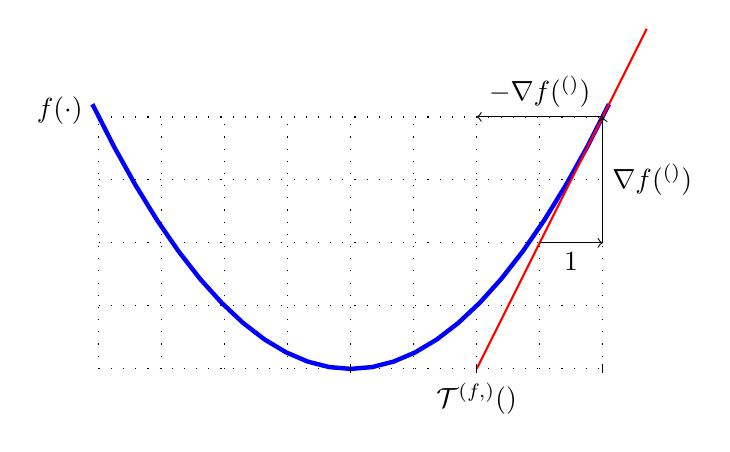
\begin{tikzpicture}[scale=0.8]
			 \draw[loosely dotted] (-4,0) grid (4,4);
			 \draw[blue, ultra thick, domain=-4.1:4.1] plot (\x,  {(1/4)*\x*\x});
			 \draw[red, thick, domain=2:4.7] plot (\x,  {2*\x - 4});
			 \draw[<-] (4,4) -- node[right] {$\nabla f(\weights^{(\itercntr)})$} (4,2);
			 \draw[->] (4,4) -- node[above] {$-\lrate \nabla f(\weights^{(\itercntr)})$} (2,4);
			 \draw[<-] (4,2) -- node[below] {$1$} (3,2) ;
			 %\draw[->] (-4.25,0) -- (4.25,0) node[right] {$a$};
			 \node[left] at (-4.1, 4.1) {$f(\cdot)$}; 
			 \draw[shift={(0,0)}] (0pt,2pt) -- (0pt,-2pt) node[below] {$\overline{\weights}$};
			 \draw[shift={(4,0)}] (0pt,2pt) -- (0pt,-2pt) node[below] {$\weights$};
			 \draw[shift={(2,0)}] (0pt,2pt) -- (0pt,-2pt) node[below] {$\mathcal{T}^{(f,\lrate)}(\weights)$};
		 \end{tikzpicture}
	 \end{center}
	 \caption{El paso básico de \gls{gradient} \eqref{equ_def_gd_basic_dict} mapea un vector $\weights$ 
	 al vector actualizado $\weights'$. Define un operador 
	 $\mathcal{T}^{(f,\lrate)}(\cdot): \mathbb{R}^{\nrfeatures} \rightarrow \mathbb{R}^{\nrfeatures}:
	  \weights \mapsto \widehat{\weights}$.}
	 \label{fig_basic_GD_step_single_dict}
 \end{figure}
 Nótese que el paso de \gls{gradient} \eqref{equ_def_gd_basic_dict} optimiza localmente - 
 en una \gls{neighborhood} cuyo tamaño está determinado por el \gls{stepsize} $\lrate$ - una aproximación lineal 
 de la función $f(\cdot)$. Un  \gls{generalization} natural de \eqref{equ_def_gd_basic_dict} es optimizar localmente
 la función misma - en lugar de su aproximación lineal - de tal manera que:
 \begin{align} 
 \label{equ_approx_gd_step_dict}
 \widehat{\weights} = \argmin_{\weights' \in \mathbb{R}^{\dimlocalmodel}} f(\weights')\!+\!(1/\lrate)\normgeneric{\weights-\weights'}{2}^2. 
 \end{align}
 Intencionalmente usamos el mismo símbolo $\lrate$ para el parámetro en \eqref{equ_approx_gd_step_dict} 
 que en el \gls{stepsize} de \eqref{equ_def_gd_basic_dict}. Mientras mayor sea el valor de $\lrate$ en 
 \eqref{equ_approx_gd_step_dict}, más progreso hará la actualización en la reducción del valor de la función $f(\widehat{\weights})$. 
 Nótese que, al igual que el paso de \gls{gradient}  \eqref{equ_def_gd_basic_dict}, 
 la actualización \eqref{equ_approx_gd_step_dict} también define un operador (típicamente no lineal)  
 parametrizado por la función $f(\cdot)$ y el parámetro $\lrate$. Para una función \gls{convex}  
 $f(\cdot)$, este operador es conocido como el \gls{proxop} de $f(\cdot)$ \cite{ProximalMethods}. 
 },first={paso de gradiente},text={paso de gradiente}}


 \newglossaryentry{proxop}{name={operador proximal},description={Dada una funcion \gls{convex}\index{operador proximal}   
 $f(\weights')$, definimos su operador proximal como \cite{ProximalMethods,Bauschke:2017} 
$$\proximityop{f(\cdot)}{\weights}{\rho}\defeq \argmin_{\weights' \in \mathbb{R}^{\dimlocalmodel}} \bigg[ f(\weights')\!+\!(\rho/2) \normgeneric{\weights- \weights'}{2}^{2}\bigg] \mbox{ with } \rho > 0. $$ 
Como se ilustra en la Figura \ref{fig_proxoperator_opt_dict}, evaluar el operador proximal 
equivale a minimizar una variante penalizada de $f(\weights')$. El término de penalización es 
la distancia euclidiana cuadrada escalada hacia un vector dado $\weights$ (que es la entrada del operador proximal). 
%\Gls{convex} functions for which the proximal operator can be computed efficiently 
%is sometimes referred to as \emph{proximable} or \emph{simple} \cite{Condat2013}. 
El operador proximal puede interpretarse como una \gls{generalization} del \gls{gradstep}, definido 
para una función \gls{smooth} y \gls{convex} $f(\weights')$. De hecho, realizar un 
\gls{gradstep} con \gls{stepsize} $\lrate$ en el vector actual $\weights$ 
es lo mismo que aplicar el \gls{proxop}de la función $\tilde{f}(\weights')= \big( \nabla f(\weights)\big)^{T} (\weights'-\weights)$ 
y usar $\rho=1/\lrate$.
	\begin{figure}[H]
	\begin{center}
		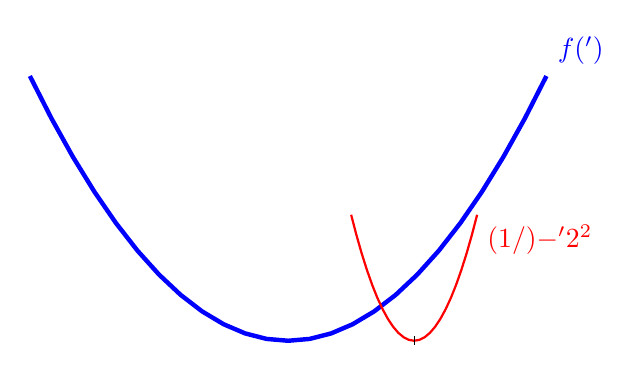
\begin{tikzpicture}[scale=0.8]
			% Original quadratic function
			\draw[blue, ultra thick, domain=-4.1:4.1] plot (\x, {(1/4)*\x*\x}) node[above right] {$f(\weights')$};		
			% Quadratic function with larger curvature, centered at w = 2
			\draw[red, thick, domain=1:3] plot (\x, {2*(\x - 2)*(\x - 2)}) node[below right] {$(1/\lrate)\normgeneric{\weights-\weights'}{2}^{2}$};
			% Axes
			% Minimum point of second curve
			\draw[shift={(2,0)}] (0pt,2pt) -- (0pt,-2pt) node[below] {$\weights$};
			%\node at (2,0.5) [anchor=north] {$\weights$};
		\end{tikzpicture}
	\end{center}
	\caption{Un \gls{gradstep} generalizado actualiza un vector $\weights$ minimizando una versión penalizada 
		de la función $f(\cdot)$. El término de penalización es la distancia euclidiana cuadrada escalada entre 
		la variable de optimización $\weights'$ y el vector dado $\weights$.\label{fig_proxoperator_opt_dict}}
\end{figure}
},first={operador proximal},text={operador proximal}}

\newglossaryentry{proximable}{name={proximable},description={Una funcion \index{proximable} 
\gls{convex} para la cual el \gls{proxop} puede calcularse de manera eficiente 
se denomina a veces proximable o simple \cite{Condat2013}.},
first={proximable},text={proximable}

}


\newglossaryentry{connected}
		{name={grafo conexo},
			description={
				Un \gls{graph} no dirigido\index{grafo conexo} $\graph=\pair{\nodes}{\edges}$ es conexo si todo subconjunto no vacío $\nodes' \subset \nodes$
				tiene al menos una arista que lo conecta con $\nodes \setminus \nodes'$.
			},
			first={grafo conexo},text={grafo conexo}
		}
	
	

	

\newglossaryentry{mvndist}{name ={distribución normal multivariante},description=
	{
		La distribución normal multivariante\index{distribución normal multivariante} $\mvnormal{\vm}{\mC}$ es una
		familia importante de \gls{probdist}s para una \gls{rv} continua $\featurevec \in \mathbb{R}^{\nrfeatures}$ \cite{BertsekasProb,GrayProbBook,Lapidoth09}.
		Esta familia está parametrizada por la \gls{mean} $\vm$ y la \gls{covmtx} $\mC$ de $\featurevec$.
		Si la \gls{covmtx} es invertible, la \gls{probdist} de $\featurevec$ es
		$$p(\featurevec) \propto \exp\bigg(-(1/2) \big( \featurevec - \vm \big)^{T} \mC^{-1} \big( \featurevec - \vm \big) \bigg).$$
		},
		first={distribución normal multivariante},text={distribución normal multivariante}
		}
		
		\newglossaryentry{statasp}{name ={aspectos estadísticos}, description={Por aspectos estadísticos\index{aspectos estadísticos} 
				de un método de \gls{ml},  nos referimos a las propiedades de la \gls{probdist} de su salida bajo 
				un \gls{probmodel} para los \gls{data} introducidos en el método.},first={aspectos estadísticos},text={aspectos estadísticos}}

				\newglossaryentry{compasp}{name ={aspectos computacionales}, description={Por aspectos 
				computacionales\index{aspectos computacionales} de un método de \gls{ml}, nos referimos principalmente a los recursos 
				computacionales requeridos para su implementación.
				Por ejemplo, si un método de \gls{ml} utiliza técnicas 
				de optimización iterativas para resolver \gls{erm}, sus aspectos computacionales incluyen: 1) cuántas 
				many operaciones aritméticas se necesitan para implementar una sola iteración(\gls{gradstep}); 
				y 2) cuántas iteraciones se requieren para obtener \gls{modelparams} útiles. Un ejemplo 
				importante de técnica de optimización iterativa es el  \gls{gd}.}, first={aspectos computacionales},text={aspectos computacionales}}
		
		\newglossaryentry{zerooneloss}{name={$\bf 0/1$ loss},
			description={La \gls{loss} $0/1$ \index{$0/1$ loss} $\lossfunczo{\pair{\featurevec}{\truelabel}}{\hypothesis}$ 
				mide la calidad de un \gls{classifier} $\hypothesis(\featurevec)$ que genera una 
				\gls{prediction} $\predictedlabel$ (por ejemplo, mediante un umbral como en \eqref{equ_def_threshold_bin_classifier_dict}) 
				para la \gls{label} $\truelabel$ de un \gls{datapoint} con \gls{feature}s $\featurevec$. Es igual a $0$ si 
				la \gls{prediction} es correcta, es decir, 
			$\lossfunczo{\pair{\featurevec}{\truelabel}}{\hypothesis}=0$ cuando $\predictedlabel=\truelabel$. Es igual 
			a $1$ si la \gls{prediction} es incorrecta, es decir, $\lossfunczo{\pair{\featurevec}{\truelabel}}{\hypothesis}=1$ 
			cuando $\predictedlabel\neq\truelabel$.},
			sort=zerooneloss, 
		   first={$0/1$ loss},text={$0/1$ loss}}
		
		\newglossaryentry{probability}{name={probabilidad},
			description={Asignamos \index{probabilidad} un valor de probabilidad, típicamente elegido en el 
				intervalo $[0,1]$, a cada evento que pueda ocurrir en un experimento aleatorio \cite{KallenbergBook,BertsekasProb,BillingsleyProbMeasure,HalmosMeasure}.},
				first={probabilidad},text={probabilidad}}


				\newglossaryentry{underfitting}{name={subajuste},
				description={Consideremos\index{subajuste} un método de \gls{ml} que utiliza \gls{erm} para aprender una \gls{hypothesis}
				con el \gls{minimum} \gls{emprisk} en un \gls{trainset} dado.
				Dicho método presenta subajuste del \gls{trainset} si no es capaz de aprender una \gls{hypothesis}
				con un \gls{emprisk} suficientemente pequeño sobre el \gls{trainset}.
				Si un método sufre de subajuste, típicamente tampoco podrá aprender una \gls{hypothesis}
				con un \gls{risk} pequeño.},
				first={subajuste},text={subajuste}
					}

\newglossaryentry{overfitting}{name={sobreajuste},description={Consideremos\index{overfitting} un 
		método de \gls{ml} que utiliza \gls{erm} para aprender una \gls{hypothesis} con el \gls{minimum} \gls{emprisk} en 
		un \gls{trainset} dado. Dicho método presenta sobreajuste del \gls{trainset} si aprende 
		una \gls{hypothesis} con un \gls{emprisk} pequeño sobre el \gls{trainset} pero una \gls{loss} significativamente mayor fuera de él \gls{trainset}.},first={sobreajuste},text={sobreajuste}}

		\newglossaryentry{gdpr}{name={reglamento general de protección de datos (RGPD)},description={
			El\index{reglamento general de protección de datos (RGPD)} RGPD
			fue promulgado por la Union Europea (EU), y entró en efecto el 25 de Mayo de 2018 \cite{GDPR2016}. 
			Protege la privacidad y los derechos sobre los \gls{data} de los individuos dentro de la EU. 
			El RGPD tiene implicaciones significativas sobre cómo se recopilan, almacenan y utilizan los \gls{data} en aplicaciones de \gls{ml}.
			Las disposiciones clave incluyen:
			\begin{itemize}
				\item \Gls{dataminprinc}: los sistemas de \gls{ml} deben utilizar únicamente la cantidad necesaria de  
				\gls{data} personal para su propósito.
				\item \Gls{transparency} y \gls{explainability}: los sistemas de \gls{ml} deben permitir a sus usuarios comprender 
				cómo se toman las decisiones que los afectan.
				\item Derechos del titular de los datos \Gls{data}:los usuarios deben tener la posibilidad de acceder, rectificar y eliminar sus \gls{data}, así como oponerse a decisiones automatizadas y perfiles.
				\item Responsabilidad: las organizaciones deben garantizar una seguridad robusta de los \gls{data} y demostrar 
				cumplimiento mediante documentación y auditorías periódicas.
			\end{itemize}
			}, 
	first={reglamento general de protección de datos (RGPD)},text={RGPD}}

\newglossaryentry{gaussrv}{name={variable aleatoria gaussiana (VA gaussiana)},description={
		Una \index{variable aleatoria gaussiana (VA gaussiana)} \gls{rv} gaussiana estándar es una \gls{rv} 
		real $x$ con \gls{pdf} \cite{papoulis,BertsekasProb,GrayProbBook}
		\begin{equation}
			\nonumber
			p(x) = \frac{1}{\sqrt{2\pi}} \exp^{-x^2/2}. 
		\end{equation}
		Dada una \gls{rv} gaussiana estándar $x$, podemos construir una \gls{rv} gaussiana general $x'$ con 
		\gls{mean} $\mu$ y \gls{variance} $\sigma^2$ mediante $x' \defeq \sigma (x+\mu)$. La \gls{probdist} de una 
		\gls{rv} gaussiana se conoce como distribución normal, denotada $\mathcal{N}(\mu,\sigma)$.  \\ 
		Un vector aleatorio gaussiano $\featurevec \in \mathbb{R}^{\featuredim}$ con 
		\gls{covmtx} $\mathbf{C}$ y \gls{mean} ${\bm \mu}$ puede construirse como 
		$\featurevec \defeq \mathbf{A} \big( \vz + {\bm \mu} \big)$. Aquí, $\mA$ 
		es cualquier matriz que satisface $\mA\mA^{T} = \mC$ y $\vz \defeq \big( z_{1},\ldots,z_{\featuredim} \big)^{T}$
		es un vector cuyos elementos son \gls{iid} gaussianas estándar \gls{rv}s $z_{1},\ldots,z_{\featuredim}$. Los procesos aleatorios gaussianos generalizan
		los vectores aleatorios gaussianos aplicando transformaciones lineales a 
		a secuencias infinitas de \gls{rv}s gaussianas estándar \cite{Rasmussen2006Gaussian}.\\
		Las \gls{rv}s gaussianas se utilizan ampliamente como \gls{probmodel}s en el análisis estadístico de métodos de \gls{ml}.
		Su importancia se debe, en parte, al teorema del límite central, que establece que el promedio de un número creciente de \gls{rv}s independientes
		(aunque no sean gaussianas) converge a una \gls{rv} gaussiana \cite{ross2013first}. 
},first={variable aleatoria gaussiana (VA gaussiana)},text={VA gaussiana}
}

\newglossaryentry{trustAI}{name={inteligencia artificial confiable (IA confiable)},description=
		{Además de los \gls{compasp} y los \gls{statasp}, un tercer aspecto principal 
		en el diseño de métodos de \gls{ml} es su confiabilidad\index{inteligencia artificial confiable (IA confiable)} \cite{pfau2024engineeringtrustworthyaideveloper}. 
		La Unión Europea ha propuesto siete requisitos clave (KRs) para una \gls{ai} confiable 
		(que típicamente se basa en métodos de \gls{ml}) \cite{ALTAIEU}: 
	\begin{enumerate}[label=\arabic*)]
		\item KR1 - Agencia y supervisión humana;
		\item KR2 - Robustez técnica y seguridad;
		\item KR3 - Privacidad y gobernanza de los \gls{data};
		\item KR4 - Transparencia;
		\item KR5 - Diversidad, no discriminación y equidad; 
		\item KR6 - Bienestar social y ambiental;
		\item KR7 - Responsabilidad. 
	\end{enumerate}
	},first={inteligencia artificial confiable (IA confiable)},text={trustworthy AI}}

\newglossaryentry{sqerrloss}{name={pérdida de error cuadrático},description={La \gls{loss} de
	error cuadrático\index{pérdida de error cuadrático} mide el error de \gls{prediction} de una 
	\gls{hypothesis} $\hypothesis$ al predecir una \gls{label} numérica $\truelabel \in \mathbb{R}$ 
	a partir de las \gls{feature}s $\featurevec$ de un \gls{datapoint}. Se define 
como 
\begin{equation} 
\nonumber
%	\label{equ_squared_loss_gls}
\lossfunc{(\featurevec,\truelabel)}{\hypothesis} \defeq \big(\truelabel - \underbrace{\hypothesis(\featurevec)}_{=\predictedlabel} \big)^{2}. 
\end{equation} 
},first={pérdida de error cuadrático},text={pérdida de error cuadrático}}


\newglossaryentry{projection}{name={proyección}, 
  description={Consideremos\index{proyección} un subconjunto $\paramspace \subseteq \mathbb{R}^{\dimlocalmodel}$ del 
   \gls{euclidspace} de dimensión $\dimlocalmodel$. Definimos la proyección $\projection{\paramspace}{\weights}$
   de un vector $\weights \in \mathbb{R}^{\dimlocalmodel}$ sobre $\paramspace$ como
	\begin{equation} 
	  \label{equ_def_proj_generic_dict}
	  \projection{\paramspace}{\weights} = \argmin_{\weights' \in \paramspace} \normgeneric{\weights - \weights'}{2}. 
	\end{equation}
	 En otras palabras, $\projection{\paramspace}{\weights}$ es el vector en $\paramspace$ más cercano a $\weights$. 
	 La proyección está bien definida solo para aquellos subconjuntos $\paramspace$ para los cuales existe el \gls{minimum} anterior \cite{BoydConvexBook}.},
	 first={proyección},text={proyección}}


	 \newglossaryentry{projgd}{name={descenso por gradiente proyectado (GD proyectado)},
	 description={Consideremos un método basado en \gls{erm} que utiliza un \gls{model} parametrizado con  
	 un \gls{paramspace} $\paramspace \subseteq \mathbb{R}^{\dimlocalmodel}$. Aun si la
	 \gls{objfunc} de \gls{erm} es \gls{smooth}, no podemos usar el \gls{gd} básico, ya 
	 ya que este no toma en cuenta las restricciones sobre la variable de optimización (es decir, los \gls{modelparams}). 
	 El \gls{gd} proyectado\index{descenso por gradiente proyectado (GD proyectado)} 
	 extiende el \gls{gd} básico para controlar restricciones sobre la variable de optimización(es decir, los \gls{modelparams}). 
	 Una sola iteración del \gls{gd} proyectado consiste primero en realizar un \gls{gradstep} 
	 y luego proyectar el resultado sobre el \gls{paramspace}.
	 \begin{figure}[H]
		 \begin{center}
			 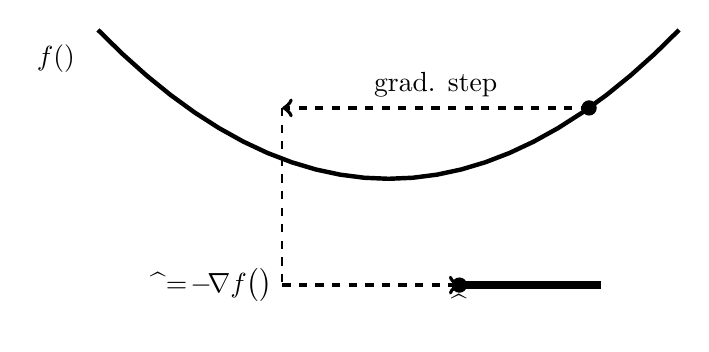
\begin{tikzpicture}[scale=0.9]
				 \node [right] at (-5.1,1.7) {$f(\weights)$} ;
				 \draw[ultra thick, domain=-4.1:4.1] plot (\x,  {(1/8)*\x*\x});
			 %	\draw[dashed, thick, domain=1:3.6] plot (\x,  {\x - 1}) node[right] {$ f\big(\weights^{(\itercntr)}\big)\!+\!\big(\weights\!-\!\weights^{(\itercntr)}\big)^{T} \nabla f\big(\weights^{(\itercntr)}\big)$};
				 \draw [fill] (2.83,1) circle [radius=0.1] node[right] {$\weights$};
				 \draw[line width =0.5mm,dashed,->] (2.83,1) -- node[midway,above] {grad. step} (-1.5,1);
				 \draw[line width =0.2mm,dashed] (-1.5,1) --(-1.5,-1.5)  node [below, left]{$\widehat{\weights}=\weights\!-\!\lrate \nabla f\big(\weights\big)$} ;
				 \draw[line width =0.5mm,dashed,->] (-1.5,-1.5)  -- node[midway,above] {} (1,-1.5) ; 
				 \draw [fill] (1,-1.5) circle [radius=0.1] node[below] {$\projection{\paramspace}{\widehat{\weights}}$};
				 \draw[line width=1mm] (1,-1.5) -- (3,-1.5) node[midway, above] {$\paramspace$};
			 \end{tikzpicture}
			 \vspace*{-5mm}
		 \end{center}
		 \caption{\gls{gd} proyectado amplía un \gls{gradstep} básico con una \gls{projection} de regreso 
		 al conjunto de restricciones $\paramspace$.}
		 \label{fig_projected_GD_dict}
	 \end{figure}},first={descenso por gradiente proyectado (GD proyectado)},text={GD proyectado}}
	 

	 \newglossaryentry{diffpriv}
	 {name=privacidad diferencial (DP),
	  description={
		  Consideremos\index{differential privacy (DP)} un método de \gls{ml} $\algomap$ que recibe como entrada un \gls{dataset} (por ejemplo, el \gls{trainset} 
		  usado para \gls{erm}) y entrega una salida $\algomap(\dataset)$. La salida 
		  puede ser los \gls{modelparams} aprendidos o las \gls{prediction}es para ciertos \gls{datapoint}s. 
		  DP es una medida precisa de la \gls{privleakage} ocasionada al revelar dicha salida.
		 Aproximadamente, un método de \gls{ml} es diferencialmente privado si la \gls{probdist} 
		  de la salida $\algomap(\dataset)$ no cambia significativamente cuando se modifica el \gls{sensattr} 
		  de un solo \gls{datapoint} del \gls{trainset}. Nótese que la DP 
		  se basa en un \gls{probmodel} para un método de \gls{ml}, es decir, interpretamos su salida $\algomap(\dataset)$ 
		  como la \gls{realization} de un \gls{rv}. La aleatoriedad en la salida puede asegurarse añadiendo intencionalmente la
		  \gls{realization} de una \gls{rv} auxiliar (ruido) a la salida del método de  \gls{ml}.
		 }, 
		 first = {privacidad diferencial (DP)}, text={DP} 
	 }
\newglossaryentry{stability}
{name={stability},
	description={
		Stability\index{stability} is a desirable property of a \gls{ml} method $\algomap$ that maps a 
		\gls{dataset} $\dataset$ (e.g., a \gls{trainset}) to an output $\algomap(\dataset)$, such as learned 
		\gls{modelparams} or the \gls{prediction} for a specific \gls{datapoint}. Intuitively, $\algomap$ is 
		stable if small changes in the input \gls{dataset} $\dataset$ lead to small changes in the 
		output $\algomap(\dataset)$. Several formal notions of stability exist that enable bounds 
		on the \gls{generalization} error or \gls{risk} of the method; see \cite[Ch.~13]{ShalevMLBook}.
		To build intuition, consider the three datasets depicted in Fig.~\ref{fig_three_data_stability}, each 
		of which is equally likely under the same \gls{data}-generating \gls{probdist}. Since the 
		optimal \gls{modelparams} are determined by this underlying \gls{probdist}, an accurate 
		\gls{ml} method $\algomap$ should return the same (or very similar) output $\algomap(\dataset)$ 
		for all three \gls{dataset}. In other words, any useful $\algomap$ must be robust to 
		variability in sample \gls{realization}s from the same \gls{probdist}, i.e., it must be stable. 
		\begin{figure}[htbp]
			\centering
			\begin{tikzpicture}
				\begin{axis}[
				%title={Stem Plots of 3 Datasets},
				    axis lines=none,
					xlabel={$\sampleidx$},
					ylabel={},
					legend pos=north west,
					ymin=0, ymax=10,
					xtick={1,2,3,4,5},
				%	ymajorgrids=true,
					grid style=dashed,
					every axis plot/.append style={very thick}
					]
					% Dataset 1
					\addplot+[only marks,mark=*] coordinates {
						(1,2) (2,4) (3,3) (4,5) (5,7)
					};
				%	\addlegendentry{$\dataset^{(*)}$}
					% Dataset 2
					\addplot+[only marks,mark=square*] coordinates {
						(1,3) (2,2) (3,6) (4,4) (5,5)
					};
				%	\addlegendentry{$\dataset^{(\square)}$}
					% Dataset 3
					\addplot+[only marks,mark=triangle*] coordinates {
						(1,5) (2,7) (3,4) (4,6) (5,3)
					};
				%	\addlegendentry{$\dataset^{(\triangle)}$}
				\end{axis}
			\end{tikzpicture}
			\caption{Three \gls{dataset}s $\dataset^{(*)}$, $\dataset^{(\square)}$, and $\dataset^{(\triangle)}$, 
				each sampled independently from the same \gls{data}-generating \gls{probdist}. A stable \gls{ml} 
				method should return similar outputs when trained on any of these \gls{dataset}s. \label{fig_three_data_stability}}
		\end{figure}
		}, 
	first = {stability}, text={stability} 
}

\newglossaryentry{privprot}
{name=protección de la privacidad,
    description={Consideremos\index{protección de la privacidad} un método de \gls{ml}  $\algomap$ que recibe como entrada 
	 una \gls{dataset} $\dataset$ y entega una salida $\algomap(\dataset)$. La salida 
	 puede ser los \gls{modelparams} aprendidos $\widehat{\weights}$ o una \gls{prediction} 
	 $\learnthypothesis(\featurevec)$ obtenida para un \gls{datapoint} específico con \gls{feature}s 
	 $\featurevec$. Muchas aplicaciones importantes de \gls{ml} involucran \gls{datapoint}s 
		que representan a personas. Cada \gls{datapoint} se caracteriza por \gls{feature}s $\featurevec$, 
		posiblemente una \gls{label} $\truelabel$, y un \gls{sensattr} $\sensattr$ (por ejemplo, un diagnóstico medico). 
		Mas o menos, la protección de la privacidad significa que debería ser imposible inferir, de la salida $\algomap(\dataset)$, 
		cualquier \gls{sensattr}s de los \gls{datapoint}s en $\dataset$. Matemáticamente, la protección de privacidad requiere que  
		el mapeo $\algomap(\dataset)$ no sea invertible. En general, el solo hacer que  $\algomap(\dataset)$ no sea invertible 
		no es suficiente. Necesitamos que sea suficientemente no invertible. 
	}, 
	first = {protección de la privacidad}, text={protección de la privacidad} 
}

\newglossaryentry{privleakage}
{
	name=filtración de privacidad,
	description={Consideremos\index{privacy leakage} una aplicacion de \gls{ml} que procesa un
	\gls{dataset} $\dataset$ y produce una salida, como las \gls{prediction}es 
	obtenidas para nuevos \gls{datapoint}s. Se produce una filtración de privacidad 
	cuando la salida contiene información privada sobre un \gls{feature} de un 
	\gls{datapoint} (que podría representar a una persona) en $\dataset$. Basado en la \gls{probmodel} 
	para la generacion de los \gls{data}, podemos medir la filtración de privacidad usando la \gls{mutualinformation} 
	entre la salida y la \gls{feature} sensible. Otra medida cuantitativa de la filtración de privacidad 
	es la \gls{diffpriv}. Las relaciones entre las diferentes medidas de filtración de privacidad han sido estudiadas en la literatura (véa \cite{InfThDiffPriv}). 
	}, 
	first = {filtración de privacidad}, text={filtración de privacidad} 
}



\newglossaryentry{probmodel}
{
	name=modelo probabilístico,
	description={Un \gls{model} probabilístico\index{modelo probabilístico} interpreta los \gls{datapoint}s 
		como \gls{realization}es de \gls{rv}s con una \gls{probdist} conjunta. Esta \gls{probdist} conjunta típicamente 
		incluye \gls{parameters} que deben seleccionarse manualmente or o aprenderse usando métodos de inferencia estadística  
		como la estimación por \gls{maxlikelihood} \cite{LC}. }, 
	first = {modelo probabilístico}, text={modelo probabilístico} 
}



\newglossaryentry{mean}
{
	name=media,
	description={La\index{media} \gls{expectation} $\expect \{ \featurevec \}$ de una \gls{rv} numérica $\featurevec$.}, 
		first = {media}, text={media} 
}

\newglossaryentry{variance}
{
	name={varianza},
	description={La\index{varianza} varianza de una \gls{rv} real $\feature$ se define como la \gls{expectation} 
		$\expect\big\{ \big( x - \expect\{x \} \big)^{2} \big\}$ de la diferencia cuadrada entre $\feature$ 
		y su \gls{expectation} $\expect\{x \}$. Extendemos esta definición a \gls{rv}s vectoriales$\featurevec$ 
		como $\expect\big\{ \big\| \featurevec - \expect\{\featurevec \} \big\|_{2}^{2} \big\}$.} ,
		first={varianza},text={varianza} 
}

\newglossaryentry{nn}
{
	name={vecino más cercano (NN)},
	description={Los métodos de vecino más cerano (NN)\index{vecino más cercano (NN)} aprenden una \gls{hypothesis} 
		$\hypothesis: \featurespace \rightarrow \labelspace$ cuyo valor $\hypothesis(\featurevec)$ 
		se determina únicamente por los \gls{neighbors} más cercanos dentro de un \gls{dataset}. Distintos 
		métodos usan diferentes medidas para determinar los \gls{neighbors} más cercanos. Si los \gls{datapoint}s 
		se caracterizan por \gls{featurevec}s numéricos, podemos usar la distancia euclidiana como medida.  
		the metric.},
	first={vecino más cercano (NN)},text={NN} 
}

\newglossaryentry{neighborhood}
{
	name={entorno},
	description={El\index{entorno} entorno de un nodo $\nodeidx \in \nodes$ es 
	el subconjunto de nodos constituido por los \gls{neighbors} de $\nodeidx$.},
	first={entorno},text={entorno} 
}

\newglossaryentry{neighbors}
{
	name={vecinos},
	description={Los\index{vecinos} vecinos de un nodo $\nodeidx \in \nodes$ 
	dentro de un \gls{empgraph} son los nodos $\nodeidx' \in \nodes \setminus \{ \nodeidx\}$ conectados con $\nodeidx$ por una arista.},
	first={vecinos},text={vecinos} 
}

\newglossaryentry{bias}
{
	name={sesgo},
	description={Consideremos\index{sesgo} un método de \gls{ml} que utiliza un \gls{hypospace} $\hypospace$ parametrizado. 
		Este aprende los \gls{modelparams} $\weights \in \mathbb{R}^{\dimlocalmodel}$ utilizando el \gls{dataset} $$ \dataset=\big\{ \pair{\featurevec^{(\sampleidx)}}{\truelabel^{(\sampleidx)}} \big\}_{\sampleidx=1}^{\samplesize}.$$ 
		Para analizar las propiedades del método de \gls{ml}, típicamente interpretamos los \gls{datapoint}s como \gls{realization}es 
		de \gls{iid} \gls{rv}s, $$ \truelabel^{(\sampleidx)} = \hypothesis^{(\overline{\weights})}\big( \featurevec^{(\sampleidx)} \big) + \bm{\varepsilon}^{(\sampleidx)}, \sampleidx=1,\ldots,\samplesize.$$ 
		Entonces podemos interpetar el método de \gls{ml} como un estimador $\widehat{\weights}$ 
		calculado a partir de $\dataset$ (por ejemplo, resolviendo \gls{erm}). El sesgo (cuadrado) del estimador $\widehat{\weights}$ 
		se define como $\biasterm^{2} \defeq \big\| \expect \{ \widehat{\weights}  \}- \overline{\weights}\big\|_{2}^{2}$. },
		first={sesgo},text={sesgo} 
}

\newglossaryentry{classification}
{name={clasificación},
description={La clasificación\index{classification} es la tarea de determinar una
	etiqueta $\truelabel$  con valor discreto para un \gls{datapoint}, basado únicamente en sus 
	 \gls{feature}s $\featurevec$. La etiqueta $\truelabel$ pertenece a un conjunto finito, como por ejemplo 
	$\truelabel \in \{-1,1\}$ o $\truelabel \in \{1,\ldots,19\}$, y representa la 
	categoría a la que pertenece el \gls{datapoint}.},
	first={clasificación},text={clasificación} 
}


\newglossaryentry{privfunnel}
{name={embudo de privacidad},
description={El\index{privacy funnel} embudo de privacidad es un método para aprender \gls{feature}s 
	amigables con la privacidad de los \gls{datapoint}s \cite{PrivacyFunnel}.},
first={embudo de privacidad},text={embudo de privacidad} 
}




\newglossaryentry{condnr}
{
	name={número de condición},
	description={El número de condición\index{número de condición} $\kappa(\mathbf{Q}) \geq 1$ de una 
		matriz definida positiva $\mathbf{Q} \in \mathbb{R}^{\featurelen \times \featurelen}$ es el cociente 
		$\alpha /\beta  $ entre el 
		mayor $\alpha$ y el menor $\beta$ \gls{eigenvalue} de 
		$\mathbf{Q}$. El número de condición es útil para el análisis de métodos de \gls{ml}. 
		La complejidad computacional de los \gls{gdmethods} para \gls{linreg} depende críticamente del número 
		de condición de la matriz $\mQ = \mX \mX^{T}$, donde $\mX$  es la \gls{featuremtx}  
		del \gls{trainset}. Es por eso que desde una perspectiva computacional, preferimos \gls{feature}s de los 
		\gls{datapoint}s que hagan que $\mQ$ tenga un número de condición cercano a $1$.},first={número de condición},text={número de condición} 
}

\newglossaryentry{classifier}
{
	name={clasificador},
	description={Un clasificador\index{clasificador} es una \gls{hypothesis} (función) $\hypothesis(\featurevec)$ 
		usada para predecir una \gls{label} que toma valores de un \gls{labelspace} finito. Podemos usar directamente 
		el valor $\hypothesis(\featurevec)$ como \gls{prediction} $\predictedlabel$ para 
		la \gls{label}. pero normalmente se usa una función $\hypothesis(\cdot)$ que entrega 
		una cantidad numérica. La \gls{prediction} es obtenida a travez de un paso de umbral. 
		Por ejemplo, en un problema de \gls{classification} binaria con \label{labelspace} $\labelspace \in  \{ -1,1\}$, 
		podríamos usar una \gls{hypothesis} de valores reales $\hypothesis(\featurevec) \in \mathbb{R}$ 
		como clasificador. Una \gls{prediction} $\predictedlabel$ puede obtenerse mediante:  
		 \begin{equation} 
		 	\label{equ_def_threshold_bin_classifier_dict}
		 	\predictedlabel =1   \mbox{ for } \hypothesis(\featurevec)\!\geq\!0 \mbox{ and } 	\predictedlabel =-1  \mbox{ otherwise.}
	 		\end{equation}
		Podemos caracterizar un clasificador mediante sus \gls{decisionregion}es $\decreg{a}$, para 
		cada valor posible de \gls{label} $a \in \labelspace$. },first={clasificador},text={clasificador} 
}

\newglossaryentry{emprisk}
{name={riesgo empírico},
 description={El \gls{risk} empírico\index{riesgo empírico} $\emprisk{\hypothesis}{\dataset}$ 
 	de una \gls{hypothesis} sobre un \gls{dataset} $\dataset$ es la \gls{loss} promedio incurrida 
 	por $\hypothesis$ al aplicarse a los \gls{datapoint}s en el $\dataset$.},
 first={riesgo empírico},text={riesgo empírico} 
}

% is it not the number of edges connected to the node instead of the neigbors?  could be the same thing, just wondering about the actual definition here. 
\newglossaryentry{nodedegree}
{name={grado de nodo},
	description={El grado\index{grado de nodo} $\nodedegree{\nodeidx}$ de un nodo $\nodeidx \in \nodes$ 
		en un \gls{graph} no dirigido, es el número de sus \gls{neighbors}, es decir, $\nodedegree{\nodeidx} \defeq \big|\neighbourhood{\nodeidx}\big|$.},
		first={grado de nodo},text={grado de nodo} 
}


\newglossaryentry{graph}
{name={grafo},
	description={Un grafo\index{graph} $\graph = \pair{\nodes}{\edges}$ es un par compuesto por un  
		conjunto de nodos $\nodes$ y un conjunto de aristas $\edges$. En su forma màs general, un grafo se 
		específica por una función que asigna a cada arista $\edgeidx \in \edges$ un par de nodos \cite{RockNetworks}. 
		Un grupo importante de grafos son los grafos no dirigidos. Un grafo simple no dirigido  
		es obtenida identificando cada arista $\edgeidx \in \edges$ con dos nodos diferentes $\{\nodeidx,\nodeidx'\}$. 
		Los grafos etiquetados asignan un peso númerico especifico \gls{weights} $\edgeweight_{\edgeidx}$ a cada 
		arista $\edgeidx \in \edges$.},first={grafo},text={grafo} 
}

\newglossaryentry{uncertainty}
{name={uncertainty},
	description={Uncertainty\index{uncertainty} refers to the degree of confidence—or 
		lack thereof—associated with a quantity such as a model prediction, parameter estimate, or 
		observed data point. In \gls{ml}, uncertainty arises from various sources, including 
		noisy data, limited training samples, or ambiguity in model assumptions. Probability theory 
		offers a principled framework for representing and quantifying such uncertainty.},
	first={uncertainty},text={uncertainty}
}

\newglossaryentry{ucb}
{name={upper confidence bound (UCB)},
	description={Consider\index{upper confidence bound (UCB)} a \gls{ml} 
		application that requires selecting, at each time step $\iteridx$, an action $\action_{\iteridx}$ 
		from a finite set of alternatives $\actionset$. The utility of selecting action $\action_{\iteridx}$ 
		is quantified by a numeric \gls{reward} signal $\reward^{(\action_{\iteridx})}$. 
		A widely used \gls{probmodel} for this type of sequential decision-making problem 
		is the stochastic multi-armed bandit setting \cite{Bubeck2012}. In this model, 
		the reward $\reward^{(\action)}$ is viewed as the \gls{realization} of a \gls{rv} 
		with unknown \gls{mean} $\mu^{(\action)}$. Ideally, we would always choose the 
		action with the largest expected \gls{reward} $\mu^{(\action)}$, but these 
		means are unknown and must be estimated from observed \gls{data}. Simply 
		choosing the action with the largest estimate $\widehat{\mu}^{(\action)}$ can 
		lead to suboptimal outcomes due to estimation uncertainty. The UCB strategy 
		addresses this by selecting actions not only based on their estimated means but 
		also by incorporating a term that reflects the uncertainty in these estimates—favouring 
		actions with high potential reward and high uncertainty. Theoretical guarantees 
		for the performance of UCB strategies,including logarithmic regret bounds, are established in \cite{Bubeck2012}.},
	first={upper confidence bound (UCB)},text={UCB} 
}

\newglossaryentry{mab}
{name={multi-armed bandit},
	description={A multi-armed bandit (MAB)\index{multi-armed bandit (MAB)} problem models 
		a repeated decision-making scenario in which, at each time step $\iteridx$, a learner must 
		choose one out of several possible actions, often referred to as arms, from a finite 
		set $\actionset$. Each arm $\action \in \actionset$ yields a stochastic \gls{reward} $\reward^{(\action)}$ 
		drawn from an unknown \gls{probdist} with \gls{mean} $\mu^{(\action)}$. 
		The learner’s goal is to maximize the cumulative \gls{reward} over time by 
		strategically balancing exploration (gathering information about 
		uncertain arms) and exploitation (selecting arms known to perform well). 
		This balance is quantified by the notion of \gls{regret}, which measures the performance 
		gap between the learner's strategy and the optimal strategy that always selects the best arm. 
		MAB problems form a foundational model in online learning, reinforcement learning, 
		and sequential experimental design \cite{Bubeck2012}.},
	first={multi-armed bandit},text={MAB}
}



\newglossaryentry{optimism in the face of uncertainty}
{name={optimismo ante la incertidumbre},
	description={Los metodos de \gls{ml}\index{optimismo ante la incertidumbre} aprenden \gls{modelparams} $\weights$ 
		de acuerdo con algún criterio de desempeño $\bar{f}(\weights)$. Sin embargo, normalmente 
		no pueden acceder directamente a $\bar{f}(\weights)$  pero dependen de una estimación (o aproximación) de $f(\weights)$. 
		Por ejemplo, los métodos basados en \gls{erm} usan la \gls{loss} promedio en un \gls{dataset} (por ejemplo, el \gls{trainset}) 
		como estimación del \gls{risk} de una \gls{hypothesis}. Usando un \gls{probmodel}, se puede construir 
		un intervalo  de confianza. 
	$\big[ l^{(\weights)},  u^{(\weights)} \big]$ para cada elección $\weights$ de los \gls{modelparams}.
	Una construcción simple es $l^{(\weights)} \defeq f(\weights) - \sigma/2$, $u^{(\weights)} \defeq f(\weights)+ \sigma/2$, 
	donde $\sigma$ representa una medida de la desviación entre $f(\weights)$ y $\bar{f}(\weights)$. 
	También se pueden usar otras construcciones del intervalo, mientras se aseguren que $\bar{f}(\weights) \in\big[ l^{(\weights)},  u^{(\weights)} \big]$ 
	con un probabilidad suficientemente alta. Siendo optimistas, elegimos los \gls{modelparams} 
	según el valor más favorable - pero realista - del criterio de desempeño $\tilde{f}(\weights) \defeq  l^{(\weights)}$. 
	Dos ejemplos de métodos de \gls{ml} que usan una construcción optimista de una \gls{objfunc} 
	son métodos de \gls{srm} \cite[Ch. 11]{ShalevMLBook} y \gls{ucb}  para decisiones secuenciales \cite[Sec. 2.2]{Bubeck2012}. 
		\begin{figure}[H]
				\begin{center}
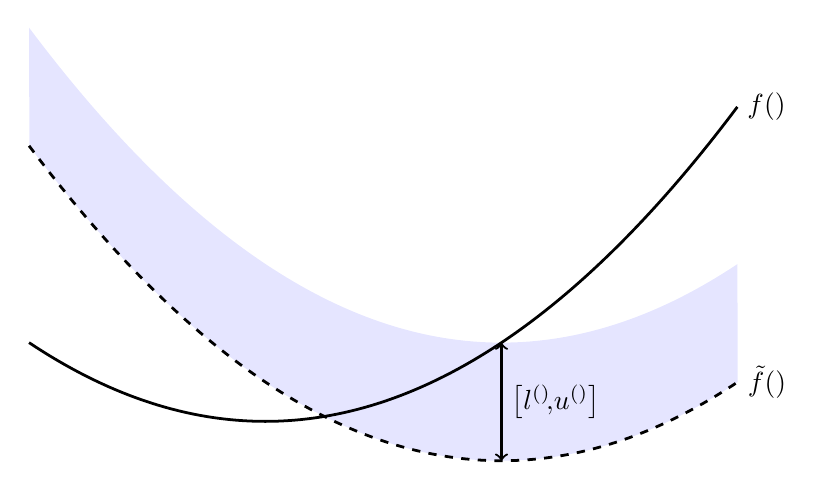
\begin{tikzpicture}[x=3cm, y=1cm]
 % Filled band around the quadratic curve with different boundary curves
\fill[blue!10] 
(-1, 5) -- plot[domain=-2:1, samples=100] ({\x+1}, {\x*\x + 1}) -- 
plot[domain=1:-2, samples=100] ({\x+1}, {\x*\x - 0.5}) -- cycle;
 \node[anchor=west] at (2, 4) {$f(\weights)$};
 \draw[line width=1, domain=-2:1, samples=100,dashed] plot  ({\x+1}, {\x*\x -0.5}) node[right] {$\tilde{f}(\weights)$};
  \draw[line width=1, domain=-1:2, samples=100] plot ({\x}, {\x*\x});
 \draw[<->, thick] (1, -0.5) -- (1, 1) node[midway, right] {$\big[ l^{(\weights)}\!,\!u^{(\weights)} \big]$};
\end{tikzpicture}
\caption{Los métodos de \gls{ml} aprenden \gls{modelparams} $\weights$ usando una estimación de $f(\weights)$ como 
	aproximación del criterio de desempeño $\bar{f}(\weights)$. Usando un \gls{probmodel}, se pueden construir intervalos de confianza $\big[ l^{(\weights)},  u^{(\weights)} \big]$ 
	que contienen $\bar{f}(\weights)$ con alta probabilidad. La mejor medida plausible del desempeño para una elección especifica $\weights$ es $\tilde{f}(\weights) \defeq l^{(\weights)}$.} 
	\end{center}
		\end{figure}},first={optimismo ante la incertidumbre},text={optimismo ante la incertidumbre} 
}

\newglossaryentry{empgraph}
{name={red de aprendizaje federado (red FL)},
	description={Una red federada\index{red de aprendizaje federado (red FL)} es un \gls{graph} no dirigido y ponderado, 
	cuyos nodos representan generadores de \gls{data} que buscan entrenar un \gls{model} local (o personalizado). 
	Cada nodo de una red federada representa un \gls{device} capaz de recopilar un \gls{localdataset}
	y, a su vez, entrenar un \gls{localmodel}. 
	Los métodos de \gls{fl} aprenden una \gls{hypothesis} local $\localhypothesis{\nodeidx}$ para
	cada nodo $\nodeidx \in \nodes$, de manera que incurra en una \gls{loss} baja sobre su \gls{localdataset}.
	,first={red de aprendizaje federado (red FL)},text={red FL} 
} }
\newglossaryentry{norm}
{name={norma},
	description={Una norma\index{norma} es una función que asigna a cada elemento (vectorial) de un espacio 
		vectorial lineal un número real no negativo. Esta función debe ser homogénea, definida positiva y debe 
		cumplir la desigualdad triangular \cite{HornMatAnalysis}. },
	first={norma},text={norma} 
}

\newglossaryentry{explanation}
{name={explicación},
	description={Un manera para hacer que los métodos de \gls{ml} sean transparentes consiste en  
		proporcionar una explicación\index{explicación} junto con la \gls{prediction} generada por el método 
		\gls{ml}. Las explicaciones pueden adoptar muchas formas diferentes. Pueden ser un texto natural
		o una medida cuantitativa que indique la importancia de atributos individuales
		de un \gls{datapoint} \cite{Molnar2019}.
 		También podemos usar formas visuales, como los mapas de intensidad usados en tareas de \gls{classification} de imágenes \cite{GradCamPaper}.},
		first={explicación},text={explicación} 
}

\newglossaryentry{risk}
{name={riesgo},
	description={Consideremos\index{riesgo} una \gls{hypothesis} $\hypothesis$ que se utiliza para predecir la \gls{label} 
		$\truelabel$ de un \gls{datapoint} a partir de sus \gls{feature}s $\featurevec$. Evaluamos 
		la calidad de una \gls{prediction} específica usando una \gls{lossfunc} $\lossfunc{(\featurevec,\truelabel)}{\hypothesis}$. 
		Si interpretamos los  \gls{datapoint}s como \gls{realization}es de \gls{rv}s \gls{iid}, 
		entonces $\lossfunc{(\featurevec,\truelabel)}{\hypothesis}$ también se convierte en una\gls{realization} 
		de una \gls{rv}. El \gls{iidasspt} nos permite definir el riesgo de una \gls{hypothesis} 
		como la \gls{expectation} de la \gls{loss} $\expect \big\{\lossfunc{(\featurevec,\truelabel)}{\hypothesis} \big\}$. 
		El riesgo de $\hypothesis$ depende tanto de la \gls{lossfunc} elegida como de la \gls{probdist} de los \gls{datapoint}s.
		},
	first={riesgo},text={riesgo} 
}

\newglossaryentry{actfun}
{name={función de activación},
	description={Cada neurona artificial dentro de una \gls{ann}\index{función de activación} se le asigna 
		una función de activación $\actfun(\cdot)$ que transforma una combinación ponderada de 
		sus entradas $\feature_{1},\ldots,\feature_{\nrfeatures}$ en un único valor de salida: 
		$a = \actfun\big(\weight_{1} \feature_{1}+\ldots+\weight_{\nrfeatures} \feature_{\nrfeatures} \big)$. 
		Cada neurona está parametrizada por los \gls{weights} $\weight_{1},\ldots,\weight_{\nrfeatures}$.},
first={función de activación},text={función de activación} 
}

\newglossaryentry{distributedalgorithm}
{name={algoritmo distribuido},
	description={Un algoritmo distribuido distributed\index{algoritmo distribuido} es un \gls{algorithm} diseñado para 
		un tipo especial de computadora: una colección de dispositivos de cómputo interconectados (o nodos). 
		Estos dispositivos se comunican y coordinan sus cálculos locales intercambiando mensajes
		a través de una red \cite{IntroDistAlg,ParallelDistrBook}. A diferencia de un \gls{algorithm} clásico,
		que se ejecuta en un solo \gls{device}, un algoritmo distribuido \gls{algorithm}  
		se ejecuta de forma concurrente en múltiples \gls{device}s con capacidades de cómputo. 
		Cada ejecución involucra tanto cálculos locales como eventos de intercambio de mensajes. 
		Una ejecución genérica podría verse así: 
		\[
		\begin{array}{l}
			\text{Node 1: } {\rm input}_1, s_1^{(1)}, s_2^{(1)}, \ldots, s_{T_1}^{(1)}, {\rm output}_1; \\
			\text{Node 2: } {\rm input}_2, s_1^{(2)}, s_2^{(2)}, \ldots, s_{T_2}^{(2)}, {\rm output}_2; \\
			\quad \vdots \\
			\text{Node N: } {\rm input}_N, s_1^{(N)}, s_2^{(N)}, \ldots, s_{T_N}^{(N)}, {\rm output}_N.
		\end{array}
		\]
		Cada \gls{device} $\nodeidx$ inicia con su entrada local y ejecuta una secuencia de 
		de cálculos intermedios $s_{\iteridx}^{(\nodeidx)}$ en instantes de tiempo discretos $\iteridx = 1, \dots, T_\nodeidx$. 
		Estos cálculos pueden depender tanto de cálculos previos locales como de mensajes recibidos de otros dispositivos.
		Uno de los usos clave de los algoritmos distribuidos es en \gls{fl}, donde una red de 
		\gls{device}s colabora para entrenar un \gls{model} personalizado por dispositivo.. 
		},
	first={algoritmo distribuido}, text={algoritmo distribuido}
}



\newglossaryentry{algorithm}
{name={algorithm},
  description={An\index{algorithm} algorithm is a precise, step-by-step specification for 
  	how to produce an output from a given input within a finite number of computational steps \cite{Cormen:2022aa}. 
    For example, an algorithm for training a \gls{linmodel} explicitly describes how to 
	transform a given \gls{trainset} into \gls{modelparams} through a sequence of \gls{gradstep}s. 
    This informal characterization can be formalized rigorously via different mathematical \gls{model}s \cite{Sipser2013}. 
    One very simple \gls{model} of an algorithm is a collection of possible executions. Each execution is a sequence:
    $${\rm input},s_1,s_2,\ldots,s_T,{\rm output}$$ 
    that respects the constraints inherent to the computer executing the algorithm.
	Algorithms may be deterministic, where each input results uniquely in a single execution,
	or randomized, where executions can vary probabilistically. Randomized algorithms 
	can thus be analyzed by modeling execution sequences as outcomes of random experiments, 
	viewing the algorithm as a stochastic process \cite{RandomizedAlgos,BertsekasProb,Gallager13}.
	Crucially, an algorithm encompasses more than just a mapping from input to output; it also includes 
	the intermediate computational steps $s_1,\ldots,s_T$. 
	%. In \textbf{online algorithms}, these intermediate computational steps  can dynamically incorporate additional input data as the execution progresses.
	},
	first={algorithm},text={algorithm} 
}

\newglossaryentry{onlinealgorithm}
{name=algoritmo en línea,
	description={
		Un algoritmo en línea\index{algoritmo en línea} es un \gls{algorithm} que procesa \gls{data} de forma incremental,
		recibiendo elementos de \gls{data} uno por uno y tomando decisiones o generando salidas inmediatamente, sin tener acceso a toda la entrada desde el inicio \cite{HazanOCO,PredictionLearningGames}.
		A diferencia de un algoritmo fuera de línea, que dispone de toda la entrada desde el comienzo, un algoritmo en línea debe lidiar con la incertidumbre del futuro y no puede cambiar decisiones pasadas.
		Puede modelarse como una ejecución del tipo:
		$${\rm init},s_1,{\rm out}_{1},{\rm in}_{2},s_2,{\rm out}_{2},\ldots,{\rm in}_{T},s_T,{\rm out}_{T}.$$
		Cada ejecución comienza en un estado inicial y alterna entre cálculos, salidas y nuevas entradas.
		Un ejemplo importante en \gls{ml} es el \gls{onlineGD}, que actualiza \gls{modelparams} conforme llegan nuevos \gls{datapoint}s.
	},
	first={algoritmo en línea},text={algoritmo en línea}
}



%\newglossaryentry{transparency}
%{name={transparency},
%	description={Transparency\index{transparency} is a key requirement for 
%		trustworthy \gls{ai} \cite{HLEGTrustworhtyAI}. In the context of ML methods, 
%		such as \gls{erm}-based methods, transparency is mainly used synonymously 
%		for \gls{explainability} \cite{gallese2023ai,JunXML2020}. However, in the wide 
%		context of \gls{ai} systems, transparency also includes providing information 
%		about limitations and reliability of the \gls{ai} system. As a point in case, \gls{logreg} provides a 
%		quantitative measure of the reliability of a \gls{classification} in the form of the value $|\hypothesis(\featurevec)|$. 
%		Transparency also includes the user interface, by requiring to clearly indicate when a user is 
%		interaction with an \gls{ai} system. Another component of transparency is the documentation 
%		of the system’s purpose, design choices, and intended use cases \cite{Shahriari2017,DatasheetData2021,10.1145/3287560.3287596}. },
%	first={transparency},text={transparency} 
%}

\newglossaryentry{transparency}
{name={transparencia},
	description={La transparencia\index{transparency} es un requisito fundamental para una 
		\gls{trustAI} confiable \cite{HLEGTrustworhtyAI}. En \gls{ml},
		suele utilizarse como sinónimo de \gls{explainability} \cite{gallese2023ai,JunXML2020}
		pero en el contexto más amplio de sistemas de \gls{ai}, 
		incluye también información sobre limitaciones, confiabilidad y uso previsto. 
		En sistemas de diagnóstico médico, se requiere informar el nivel de confianza de una \gls{prediction}.
		En aplicaciones financieras como la puntuación crediticia, las decisiones automatizadas basadas en \gls{ai}
		deben ir acompañadas de explicaciones sobre los factores que influyeron en ellas, como el nivel de ingresos o el historial crediticio. These explanations 
		Estas explicaciones permiten que las personas (por ejemplo, un solicitante de crédito) comprendan y, 
		si es necesario, impugnen decisiones automatizadas.. 
		Algunos métodos de \gls{ml} ofrecen transparencia de manera intrínseca. Por ejemplo, la \gls{logreg} 
		permite interpretar la fiabilidad de una \gls{classification} mediante el valor absoluto $|\hypothesis(\featurevec)|$. 
		Las \gls{decisiontree}s,  también son consideradas transparentes porque generan reglas comprensibles para los humanos.
		\cite{rudin2019stop}.
		La transparencia también requiere que se informe explícitamente cuando una persona está interactuando con un sistema \gls{ai}.
		Por ejemplo, los chatbots impulsados por \gls{ai} deben indicar claramente que no son humanos. 
		For example, \gls{ai}-powered chatbots should notify users that they are interacting with an 
		automated system rather than a human. Furthermore, transparency encompasses comprehensive 
		documentation detailing the purpose and design choices underlying the \gls{ai} system. 
		Además, la transparencia incluye documentación exhaustiva que detalle el propósito, las decisiones de diseño y los casos de uso previstos del sistema.
		Ejemplos de esto son las hojas de datos de \gls{model}s \cite{DatasheetData2021}
		 y las tarjetas de sistemas de \gls{ai} \cite{10.1145/3287560.3287596}, 
		 que ayudan a los desarrolladores y usuarios a entender las limitaciones y aplicaciones adecuadas de un sistema \gls{ai} \cite{Shahriari2017}.
		 },
	first={transparencia}, text={transparencia} 
}


\newglossaryentry{sensattr}
{
	name=atributo sensible,
	description={
		La \gls{ml}\index{atributo sensible} busca aprender una \gls{hypothesis} que prediga la \gls{label} de un \gls{datapoint} a partir de sus \gls{feature}s.
		En algunas aplicaciones, es crucial garantizar que la salida del sistema no permita inferir atributos sensibles de los \gls{datapoint}s.
		Qué se considera atributo sensible depende del dominio de aplicación y debe definirse explícitamente.
	},
	first={atributo sensible},text={atributo sensible}
}

\newglossaryentry{sbm}
{
	name=modelo estocástico de bloques (SBM),
	description={
		El modelo estocástico de bloques (SBM)\index{modelo estocástico de bloques (SBM)} es un \gls{model} generativo probabilístico para un \gls{graph} no dirigido $\graph = \big( \nodes, \edges \big)$ con conjunto de nodos $\nodes$ \cite{AbbeSBM2018}.
		En su forma básica, asigna aleatoriamente cada nodo $\nodeidx \in \nodes$ a una \gls{cluster} $\clusteridx_{\nodeidx} \in \{1,\ldots,\nrcluster\}$.
		Cada par de nodos distintos se conecta con \gls{probability} $p_{\nodeidx,\nodeidx'}$ que depende únicamente de sus \gls{label}s $\clusteridx_{\nodeidx}$ y $\clusteridx_{\nodeidx'}$.
		La presencia de aristas entre pares de nodos es estadísticamente independiente.
	},
	first={modelo estocástico de bloques (SBM)},text={SBM}
}


\newglossaryentry{deepnet}
{name={red profunda},
	description={Una red profunda\index{deep net} es una \gls{ann} con un número (relativamente) grande 
	de capas ocultas. El aprendizaje profundo (deep learning) es un término general para los métodos de \gls{ml} 
	que utilizan una red profunda como \gls{model}  \cite{Goodfellow-et-al-2016}.},
	first={red profunda},text={red profunda} 
}

\newcommand{\gaussiancenter}{3}

\newglossaryentry{baseline}
{name={referencia (baseline)},
    description={Consideremos\index{referencia (baseline)} un método de \gls{ml} que produce una 
    \gls{hypothesis} aprendida (o un \gls{model} entrenado) $\learnthypothesis \in \hypospace$.
	Evaluamos la calidad del \gls{model} entrenado  
	mediante el cálculo de la \gls{loss} promedio en un \gls{testset}.Pero, ¿cómo saber si ese rendimiento es lo suficientemente bueno?
	¿Cómo saber si el \gls{model} entrenado se acerca al óptimo y si tiene sentido o no invertir más recursos (como recopilación de \gls{data} o potencia computacional) para mejorarlo? 
    Para ello, es útil contar con un valor de referencia (o *baseline*) con el cual comparar el rendimiento  
    del modelo \gls{model} entrenado. Este valor puede provenir del rendimiento humano,
    como la tasa de error de dermatólogos que diagnostican cáncer mediante inspección visual de la piel \cite{SkinHumanAI}.
	Otra fuente de referencia puede ser un método de \gls{ml} ya existente que, por alguna razón, no sea adecuado para la aplicación (por ejemplo, por ser computacionalmente costoso), pero cuya tasa de error en el \gls{testset} puede servir como baseline.
	Un enfoque más fundamentado para construir una baseline es utilizar un \gls{probmodel}. En muchos casos, dado un \gls{probmodel} \gls{probmodel} $p(\featurevec,\truelabel)$,  
    podemos determinar con precisión el \gls{minimum} \gls{risk} alcanzable entre todas las hipótesis (incluso aquellas que no pertenecen al \gls{hypospace} $\hypospace$) \cite{LC}. 
    Este \gls{minimum} alcanzable se conoce como \gls{bayesrisk} y corresponde al \gls{risk} del \gls{bayesestimator} para la \gls{label} $\truelabel$ de un \gls{datapoint}, dados sus \gls{feature}s $\featurevec$.
	Dado un \gls{lossfunc} específico, el \gls{bayesestimator} (si existe) está completamente determinado por la \gls{probdist} $p(\featurevec,\truelabel)$ \cite[Cap. 4]{LC}. 
    Calcular el \gls{bayesestimator} y el \gls{bayesrisk} presenta dos desafíos principales:
    \begin{enumerate}[label=\arabic*)]
    	\item La \gls{probdist} $p(\featurevec,\truelabel)$ desconocida y debe estimarse.
    	\item Incluso si se conoce $p(\featurevec,\truelabel)$ calcular el 
		\gls{bayesrisk} puede ser computacionalmente muy costoso \cite{cooper1990computational}.
	\end{enumerate}
	Un \gls{probmodel} ampliamente utilizado es la \gls{mvndist} $\pair{\featurevec}{\truelabel} \sim \mathcal{N}({\bm \mu},{\bm \Sigma})$ 
para \gls{datapoint}s caracterizados por \gls{feature}s y \gls{label}s numéricos.
En este caso, bajo la \gls{sqerrloss}, el \gls{bayesestimator} corresponde a la \gls{mean} posterior
$\mu_{\truelabel|\featurevec}$ de la \gls{label} $\truelabel$, dado  
\gls{feature}s $\featurevec$ \cite{LC,GrayProbBook}. El \gls{bayesrisk} asociado es la 
\gls{variance} posterior
$\sigma^{2}_{\truelabel|\featurevec}$ (see Figure \ref{fig_post_baseline_dict}).
	\begin{figure}[H]
		\begin{center}
		\begin{tikzpicture}
			% Axes
			\draw[->] (-1,0) -- (7,0) node[right] {$\truelabel$}; % x-axis
			% Gaussian distribution centered at \gaussiancenter with variance 1
			\draw[thick,domain=-1:7,smooth,variable=\x] 
			  plot ({\x}, {2*exp(-0.5*((\x-\gaussiancenter)^2))});
			% Dashed line indicating the mean of the Gaussian
			\draw[dashed] (\gaussiancenter,0) -- (\gaussiancenter,2.5);
			\node[anchor=south] at ([yshift=-5pt] \gaussiancenter,2.5) {\small $\mu_{\truelabel|\featurevec}$};
			% Double arrow indicating the variance
			\draw[<->,thick] (\gaussiancenter-1,1) -- (\gaussiancenter+1,1.0);
			\node[anchor=west] at ([yshift=2pt] \gaussiancenter,1.2) {\small $\sigma_{\truelabel|\featurevec}$};
			% Posterior variance label
			%\node[anchor=south east] at (\gaussiancenter-0.5,1.8) {\small Posterior Variance};
			% x-axis marks with crosses
			  % x-axis marks with crosses
  			\foreach \x in {0.5} {
				\node[red] at (\x, 0) {\bf \large $\times$};
 			 }
  % h(x) label for the first cross
  			\node[anchor=north] at (0.5,-0.2) {\small $\learnthypothesis(\featurevec)$};
		  \end{tikzpicture}
		\end{center}
		\caption{Si los \gls{feature}s y la  \gls{label} de un \gls{datapoint} siguen una \gls{mvndist}, we 
		podemos alcanzar el \gls{minimum} \gls{risk} (bajo \gls{sqerrloss}) usando el \gls{bayesestimator} $\mu_{\truelabel|\featurevec}$ 
		para predecir el \gls{label} $\truelabel$ de un \gls{datapoint} con \gls{feature}s $\featurevec$. El
		\gls{minimum} \gls{risk} es dada por la \gls{variance} posterior $\sigma^{2}_{\truelabel|\featurevec}$. Podemos 
		usar esta cantidad como baseline para evaluar la \gls{loss} promedio del \gls{model} $\learnthypothesis$ entrenado. \label{fig_post_baseline_dict}}
	\end{figure}},
    first={referencia (baseline)},text={referencia (baseline)}
}

\newglossaryentry{spectrogram}
{name={espectrograma},
	description={
		Un\index{espectrograma} espectrograma representa la distribución tiempo-frecuencia de la energía de una señal temporal $x(t)$.  
		Intuitivamente, cuantifica la cantidad de energía de la señal presentedentro de un segmento de tiempo específico 
		$[t_{1},t_{2}] \subseteq \mathbb{R}$ y en un intervalo de frecuencia $[f_{1},f_{2}]\subseteq \mathbb{R}$. 
		Formalmente, el espectrograma de una señal se define como el módulo al cuadrado de su transformada
		de Fourier de ventana corta (STFT, en inglés) \cite{cohen1995time}.
        La Figure \ref{fig:spectrogram_dict} muestra una señal temporal junto con su espectrograma. 
	\begin{figure}[H]
		\centering
		\includegraphics[width=0.8\textwidth]{../../assets/spectrogram.png}
		\caption{Izquierda: una señal temporal compuesta por dos pulsos gaussianos modulados. Derecha: representación de intensidad de su espectrograma.
		\label{fig:spectrogram_dict}}
	\end{figure}
		La representación de intensidad del espectrograma puede considerarse como una imagen de la señal. 
		Una estrategia sencilla para la \gls{classification} de señales de audio consiste en introducir esta imagen en una 
		\gls{deepnet} desarrollada originalmente para tareas de \gls{classification} de imágenes y detección de objetos \cite{Li:2022aa}. 
		Conviene señalar que, además del espectrograma, existen otras representaciones alternativas para describir la distribución 
		tiempo-frecuencia de la energía de una señal \cite{TimeFrequencyAnalysisBoashash,MallatBook}. 
		}, 
	first={espectrograma},text={espectrograma} 
}

\newglossaryentry{graphclustering}
{name={agrupamiento en grafos},
	description={El \gls{clustering} en \gls{graph}s\index{agrupamiento en grafos} tiene como objetivo agrupar \gls{datapoint}s que están representados como nodos de un \gls{graph} $\graph$.
		Las aristas del $\graph$ representan similitudes por pares entre los \gls{datapoint}s. 
		En algunos casos, es posible cuantificar el grado de estas similitudes mediante un \gls{edgeweight} \cite{Luxburg2007,FlowSpecClustering2021}. 
		}, 
	first={agrupamiento en grafos},text={agrupamiento en grafos} 
}

\newglossaryentry{specclustering}
{name={agrupamiento espectral},
	description={El \gls{clustering} espectral \index{agrupamiento espectral} es una instancia particular del 
		\gls{graphclustering}, es decir, agrupa \gls{datapoint}s 
		representados como los nodos $\nodeidx=1,\ldots,\nrnodes$ de un \gls{graph} $\graph$. 
		El \gls{clustering} espectral utiliza los \gls{eigenvector}s de la \gls{LapMat} $\LapMat{\graph}$ 
		para construir \gls{featurevec}s $\featurevec^{(\nodeidx)} \in \mathbb{R}^{\nrfeatures}$ 
		para cada nodo (es decir, para cada \gls{datapoint}) $\nodeidx=1,\ldots,\nrnodes$. Podemos utilizar estos \gls{featurevec}s 
		como entrada para métodos de \gls{clustering} en \gls{euclidspace},como \gls{kmeans} 
		o \gls{softclustering} mediante \gls{gmm}. Mas o menos, los \gls{featurevec}s de los nodos 
		que pertenecen a un subconjunto bien conectado (o \gls{cluster}) de nodos en $\graph$ estan ubicados 
		cerca en el \gls{euclidspace} $\mathbb{R}^{\nrfeatures}$ (Vea la Figura \ref{fig_lap_mtx_specclustering_dict}). 
		\begin{figure}[H]
			\begin{center}
				\begin{minipage}{0.4\textwidth}
			\begin{tikzpicture}
				% Define the style for filled nodes
				\begin{scope}[every node/.style={circle, fill=black, inner sep=0pt, minimum size=0.3cm}]
					% Define nodes
					\node (1) at (0,0) {};
					\node (2) [below left=of 1, xshift=-0.2cm, yshift=-1cm] {};
					\node (3) [below right=of 1, xshift=0.2cm, yshift=-1cm] {};
					\node (4) [below=of 1, yshift=0.5cm] {}; % Isolated node
				\end{scope}
				% Draw edges
				\draw (1) -- (2);
				\draw (1) -- (3);
				% Add labels (separate from filled nodes)
				\node[above=0.2cm] at (1) {$\nodeidx=1$};
				\node[left=0.3cm] at (2) {$2$};
				\node[right=0.3cm] at (3) {$3$};
				\node[below=0.2cm] at (4) {$4$};
			\end{tikzpicture}
				\end{minipage} 
				\hspace*{5mm}
				\begin{minipage}{0.4\textwidth}
					\begin{equation} 
						\LapMat{\graph}\!=\!
						\begin{pmatrix} 
							2 & -1 & -1 & 0 \\ 
							-1 & 1 & 0 & 0 \\  
							-1 & 0 & 1 & 0 \\ 
							0 & 0 & 0 & 0 
						\end{pmatrix}\!=\!\mathbf{V} {\bm \Lambda} \mathbf{V}^{T}  
						\nonumber
					\end{equation} 
				\end{minipage}
				\vspace*{20mm}\\
				  \begin{minipage}{0.4\textwidth}
				\begin{tikzpicture}[scale=3]
%					% Axes
					\draw[->] (-0.2, 0) -- (1.2, 0) node[right] {$v^{(1)}_{\nodeidx}$};
					\draw[->] (0, -0.2) -- (0, 1.2) node[above] {$v^{(2)}_{\nodeidx}$};
%					
%					% Tailored tick marks and labels
%					\draw (0,0) node[below left] {$0$};
%					\draw (1/sqrt(3), 0) node[below] {$\frac{1}{\sqrt{3}}$} -- ++(0,0.05);
%					\draw (0, 1) node[left] {$1$} -- ++(0.05,0);
%					
%					 Data points
					\filldraw[blue] (0.577, 0) circle (0.03cm) node[above right] {$\nodeidx=1,2,3$};
					\filldraw[blue] (0.577, 0) circle (0.03cm); % Second point overlaps
					\filldraw[blue] (0.577, 0) circle (0.03cm); % Third point overlaps
					\filldraw[red] (0, 1) circle (0.03cm) node[above right] {$4$};
%					% Grid for reference
%					\draw[dashed, gray] (1/sqrt(3), 0) -- (1/sqrt(3), 1);
%					\draw[dashed, gray] (0, 1) -- (1, 1);
				\end{tikzpicture}
				\end{minipage} 
    		\begin{minipage}{0.4\textwidth}
										\begin{align}
											& \mathbf{V} = \big( \vv^{(1)},\vv^{(2)},\vv^{(3)},\vv^{(4)} \big) \nonumber \\
											&	\mathbf{v}^{(1)}\!=\!\frac{1}{\sqrt{3}} \begin{pmatrix} 1 \\ 1 \\ 1 \\ 0 \end{pmatrix}, \,
												\mathbf{v}^{(2)}\!=\!\begin{pmatrix} 0 \\ 0 \\ 0 \\ 1 \end{pmatrix} \nonumber 
												\end{align}
				\end{minipage} 
				\caption{\label{fig_lap_mtx_specclustering_dict} {\bf Arriba.} Izquierda: Un \gls{graph} no dirigido
					$\graph$ con cuatro nodos $\nodeidx=1,2,3,4$, donde cada nodo representa un \gls{datapoint}. Derecha: La \gls{LapMat} 
					$\LapMat{\graph}  \in \mathbb{R}^{4 \times 4}$ y su \gls{evd}. 
					{\bf Abajo.} Izquierda: Un \gls{scatterplot} de los \gls{datapoint}s usando los \gls{featurevec}s 
					$\featurevec^{(\nodeidx)} = \big( v^{(1)}_{\nodeidx},v^{(2)}_{\nodeidx} \big)^{T}$. 
					Derecha: Dos \gls{eigenvector}s $\vv^{(1)},\vv^{(2)} \in \mathbb{R}^{\nrfeatures}$ 
					correspondientes al \gls{eigenvalue} $\lambda=0$ de la \gls{LapMat} $\LapMat{\graph}$. 
					} 
			\end{center}
		\end{figure}
	\newpage}, 
	first={agrupamiento espectral},text={agrupamiento espectral} 
}
\newglossaryentry{flowbasedclustering}
{name={agrupamiento basado en flujo},
	description={El \gls{clustering} basado en flujo\index{agrupamiento basado en flujo} agrupa los nodos de un 
		\gls{graph} no dirigido aplicando el algoritmo de \gls{kmeans} sobre
		\gls{featurevec}s específicos para cada nodo. Estos \gls{featurevec}s se construyen a partir de flujos de red entre nodos 
		fuente y destino seleccionados cuidadosamente \cite{FlowSpecClustering2021}. }, 
	first={agrupamiento basado en flujo},text={agrupamiento basado en flujo} 
}



\newglossaryentry{esterr}
{name={error de estimación},
	description={Consideremos\index{error de estimación} \gls{datapoint}s, cada uno con un \gls{featurevec} $\featurevec$ y una \gls{label} 
		$\truelabel$. En algunas aplicaciones, podemos modelar la relación entre el \gls{featurevec} y la \gls{label}
		de un \gls{datapoint} como $\truelabel = \bar{\hypothesis}(\featurevec) + \varepsilon$. Aquí $\bar{\hypothesis}$ 
		representa la \gls{hypothesis} verdadera subyacente y $\varepsilon$ es un término de ruido que resume errores de modelado o etiquetado.
		El error de estimación incurrido por un método de \gls{ml} que aprende una \gls{hypothesis} $\widehat{\hypothesis}$, por ejemplo usando \gls{erm}, se define como 
		$\widehat{\hypothesis}(\featurevec) - \bar{\hypothesis}(\featurevec)$, para algún \gls{featurevec} dado. 
		En un \gls{hypospace} paramétrico, donde las \gls{hypothesis}se determinan mediante
		\gls{modelparams} $\weights$, podemos definir el error de estimación como  $\Delta \weights = \widehat{\weights} - \overline{\weights}$ \cite{kay,hastie01statisticallearning}.},
	first={error de estimación},text={error de estimación} 
}


\newglossaryentry{dob}
{name={grado de pertenencia},
	description={El grado de pertenencia\index{grado de pertenencia} es un número que indica en qué medida un \gls{datapoint} 
		pertenece a un \gls{cluster} \cite[Ch. 8]{MLBasics}. Este grado puede interpretarse 
		como una asignación blanda (*soft*) al \gls{cluster}.Los métodos de \Gls{softclustering} 
		pueden codificar el grado de pertenencia mediante un número real en el intervalo $[0,1]$. 
		El \Gls{hardclustering} se obtiene como caso extremo, cuando el grado de pertenencia solo toma los valores $0$ o $1$.
		}, 
		first={grado de pertenencia},text={grado de pertenencia} 
}

\newglossaryentry{msee}
{name={error cuadrático medio de estimación (MSEE)},
	description={Consideremos\index{error cuadrático medio de estimación (MSEE)} un método de \gls{ml} que aprende 
		\gls{modelparams} $\widehat{\weights}$ a partir de un \gls{dataset} $\dataset$. 
		Si interpretamos los \gls{datapoint}s en $\dataset$ como \gls{realization}s \gls{iid} de una \gls{rv} $\datapoint$, 
		definimos el \gls{esterr} como $\Delta \weights \defeq \widehat{\weight} - \overline{\weights}$. 
		Aquí, $\overline{\weights}$ representa los verdaderos \gls{modelparams} de la \gls{probdist} 
		de $\datapoint$. El error cuadrático medio de estimación se define como la \gls{expectation} $\expect \big\{ \big\| \Delta \weights \big\|^{2} \big\}$ del cuadrado de la 
		\gls{norm} euclidiana del \gls{esterr} \cite{LC,kay}.},
	first={error cuadrático medio de estimación (MSEE)},text={MSEE} 
}

\newglossaryentry{gtvmin}
{name={minimización de variación total generalizada (GTVMin)},
	description={La minimización de variación total generalizada (GTVMin)\index{minimización de variación total generalizada (GTVMin)} es una instancia de \gls{rerm} 
	que utiliza la \gls{gtv} de los \gls{modelparams} locales como un \gls{regularizer} \cite{ClusteredFLTVMinTSP}.},
	first={minimización de variación total generalizada (GTVMin)},text={GTVMin} 
}

\newglossaryentry{regression}
{name={regresión},
	description={Los problemas de regresión\index{regresión} se centran en la predicción de una 
		\gls{label} numérica basada únicamente en las \gls{feature}s de un \gls{datapoint} \cite[Ch. 2]{MLBasics}.},
	first={regresión},text={regresión} 
}

\newglossaryentry{acc}
{name={precisión (accuracy)},
	description={Consideremos\index{precisión (accuracy)} \gls{datapoint}s caracterizados por\gls{feature}s $\featurevec \in \featurespace$ y 
		una etiqueta categórica $\truelabel$ que toma valores de un conjunto finito \gls{labelspace} $\labelspace$. La 
		precisión de una \gls{hypothesis} $\hypothesis: \featurespace \rightarrow \labelspace$, cuando se aplica a los
		\gls{datapoint}s en un \gls{dataset} $\dataset = \big\{ \big(\featurevec^{(1)}, \truelabel^{(1)} \big), \ldots, \big(\featurevec^{(\samplesize)},\truelabel^{(\samplesize)}\big) \big\}$, 
		se define como $1 - (1/\samplesize)\sum_{\sampleidx=1}^{\samplesize} \lossfunczo{\big(\featurevec^{(\sampleidx)},\truelabel^{(\sampleidx)}\big)}{\hypothesis}$ usando la \gls{zerooneloss} $\lossfunczo{\cdot}{\cdot}$.},
	first={precisión (accuracy)},text={precisión} 
}





\newglossaryentry{expert}
{name={experto},
	description={El \gls{ml}\index{experto} tiene como objetivo aprender una \gls{hypothesis} $\hypothesis$ que prediga con precisión la \gls{label} 
		de un \gls{datapoint} basado en sus \gls{feature}s. Medimos el error de \gls{prediction} utilizando una
		\gls{lossfunc}. Idealmente, buscamos una \gls{hypothesis} que incurra en la \gls{loss} mínima
		para cualquier \gls{datapoint}. Podemos hacer este objetivo más preciso mediante el \gls{iidasspt} 
		y utilizando el \gls{bayesrisk} como referencia \gls{baseline} para la \gls{loss} promedio de una \gls{hypothesis}. 
		Una manera alternativa de obtener una\gls{baseline} es utilizar la \gls{hypothesis} $\hypothesis'$ aprendida 
		por un método de \gls{ml} existente. A esta \gls{hypothesis} $\hypothesis'$ la denominamos experto \cite{PredictionLearningGames}. Los métodos de minimización de \Gls{regret} aprenden una \gls{hypothesis}
		que incurre en una \gls{loss} comparable a la del mejor experto \cite{PredictionLearningGames,HazanOCO}.},
	first={experto},text={experto} 
}

\newglossaryentry{nfl}
{name={aprendizaje federado en red (NFL)},
	description={El aprendizaje federado en red (NFL)\index{aprendizaje federado en red (NFL)} se refiere 
		a métodos que aprenden \gls{model}s personalizados de manera distribuida. Estos métodos aprenden a partir de \gls{localdataset}s 
		que están relacionados por una estructura de red intrínseca.
		},
 first={aprendizaje federado en red (NFL)},text={NFL} 
}




\newglossaryentry{regret}
{name={arrepentimiento (regret)},
	description={El arrepentimiento\index{arrepentimiento (regret)} de una \gls{hypothesis} $\hypothesis$ en relación con otra 
		\gls{hypothesis} $\hypothesis'$, que sirve como referencia \gls{baseline}, 
		es la diferencia entre la \gls{loss} incurrida por $\hypothesis$ y la \gls{loss} 
		incurrida por $\hypothesis'$ \cite{PredictionLearningGames}. 
		La \gls{baseline} \gls{hypothesis} de referencia $\hypothesis'$ también se denomina \gls{expert}.},
	first={arrepentimiento (regret)},text={arrepentimiento (regret)} 
}

\newglossaryentry{strcvx}
{name={fuertemente convexa},
	description={Una función real \gls{differentiable} de valor continuo 
		 $f(\featurevec)$es fuertemente \gls{convex} con coeficiente $\sigma$ si cumple: $f(\vy) \geq f(\vx) + \nabla f(\vx)^{T} (\vy - \vx) + (\sigma/2) \normgeneric{\vy - \vx}{2}^{2}$ \cite{nesterov04},\cite[Sec. B.1.1]{CvxAlgBertsekas}.},
	first={fuertemente convexa},text={fuertemente convexa} 
}

\newglossaryentry{differentiable}
{name={diferenciable},
	description={Una función real $f: \mathbb{R}^{\featuredim} \rightarrow \mathbb{R}$ 
		es diferenciable\index{diferenciable} si, en cualquier punto, puede aproximarse localmente mediante una función lineal.
		La aproximación lineal local en el punto $\mathbf{x}$ es determinada por el 
		\gls{gradient} $\nabla f ( \mathbf{x})$ \cite{RudinBookPrinciplesMatheAnalysis}.},
	first={diferenciable},text={diferenciable} 
}

\newglossaryentry{gradient}
{name={gradiente},
	description={Para\index{gradiente} una función de valor real $f: \mathbb{R}^{\featuredim} \rightarrow \mathbb{R}: \weights \mapsto f(\weights)$, 
	un vector $\vg$ tal que $\lim_{\weights \rightarrow \weights'} \frac{f(\weights) - \big(f(\weights')+ \vg^{T} (\weights- \weights') \big) }{\| \weights-\weights'\|}=0$ 
	se denomina gradiente de $f$ en $\weights'$. Si existe tal vector, se denota como
	$\nabla f(\weights')$ o $\nabla f(\weights)\big|_{\weights'}$ \cite{RudinBookPrinciplesMatheAnalysis}.},
	first={gradiente},text={gradiente} 
}

\newglossaryentry{subgradient}
{name={subgradiente},
description={Para\index{subgradiente} una función de valor real $f: \mathbb{R}^{\featuredim} \rightarrow \mathbb{R}: \weights \mapsto f(\weights)$, 
		un vector $\va$ tal que $f(\weights) \geq  f(\weights') +\big(\weights-\weights' \big)^{T} \va$ se 
		se denomina subgradiente de $f$ en $\weights'$ \cite{BertCvxAnalOpt,BertsekasNonLinProgr}.},
	first={subgradiente},text={subgradiente} 
}

\newglossaryentry{fedavg}
{name={promedio federado (FedAvg)},
	description={El promedio federado (FedAvg)\index{promedio federado (FedAvg)}se refiere a un \gls{algorithm} iterativo de \gls{fl} que alterna entre entrenar \gls{localmodel}s por separado y combinar los \gls{modelparams} locales actualizados.
		El entrenamiento de los \gls{localmodel}s se implementa a través de varios pasos de \gls{stochGD} \cite{pmlr-v54-mcmahan17a}.}, 
		first = {FedAvg}, text={FedAvg} 
}

\newglossaryentry{fedprox}
{name={FedProx},
	description={FedProx\index{FedProx}  se refiere a un \gls{algorithm} iterativo de \gls{fl} que alterna entre entrenar \gls{localmodel}s por separado y combinar los \gls{modelparams} locales actualizados. 
		A diferencia de \gls{fedavg}, que utiliza \gls{stochGD} para entrenar los \gls{localmodel}s, FedProx usa un \gls{proxop}  para el entrenamiento \cite{FedProx2020}.}, 
	first = {FedProx}, text={FedProx} 
}

\newglossaryentry{relu}
{name={unidad lineal rectificada (ReLU)},
	description={La unidad lineal rectificada (ReLU)\index{unidad lineal rectificada (ReLU)} es una elección popular para la 
		\gls{actfun} de una neurona dentro de una \gls{ann}. Se define como  
		$\actfun(z) = \max\{0,z\}$, donde $z$ es la entrada ponderada de la neurona artificial.
		}, 
	first = {unidad lineal rectificada (ReLU)}, text={ReLU} 
}

\newglossaryentry{hypothesis}
{name={hipótesis},
	description={Una hipótesis\index{hipótesis} se refiere a un mapa (o función) $\hypothesis: \featurespace \rightarrow \labelspace$ que va del
		\gls{featurespace} $\featurespace$ al \gls{labelspace} $\labelspace$. 
		Dado un \gls{datapoint} con \gls{feature}s $\featurevec$, utilizamos un mapa de hipótesis $\hypothesis$
		para estimar (o aproximar) la \gls{label} $\truelabel$ mediante la \gls{prediction}  
		$\hat{\truelabel} = \hypothesis(\featurevec)$. El \Gls{ml} se centra en aprender (o encontrar) un mapa de hipótesis 
		$\hypothesis$ tal que $\truelabel \approx \hypothesis(\featurevec)$ 
		para cualquier \gls{datapoint} (con \gls{feature}s $\featurevec$ y \gls{label} $\truelabel$).},
	first={hipótesis},text={hipótesis}  
}



\newglossaryentry{vcdim}
{name={dimensión de Vapnik–Chervonenkis (dimensión VC)},
	description={La dimensión VC (Vapnik–Chervonenkis)\index{dimensión de Vapnik–Chervonenkis (dimensión VC)} de un \gls{hypospace} infinito es una medida ampliamente utilizada para su tamaño.
		Nos referimos a la literatura (vea \cite{ShalevMLBook}) para una definición precisa de la dimensión VC,
		y para una discusión de sus propiedades básicas y su uso en \gls{ml}.},
	first={dimensión de Vapnik–Chervonenkis (dimensión VC)},text={dimensión VC}  
}

\newglossaryentry{effdim}
{name={dimensión efectiva},
	description={La dimensión efectiva\index{dimensión efectiva} $\effdim{\hypospace}$ de un 
		\gls{hypospace} infinito $\hypospace$ es una medida de su tamaño. A grandes rasgos,la 
		dimensión efectiva es igual al número efectivo de \gls{modelparams} independientes y ajustables. 
		Estos \gls{parameters} pueden ser los coeficientes utilizados en un mapa lineal o los 
		\gls{weights} y términos de sesgo de una \gls{ann}.},
	first={dimensión efectiva},text={dimensión efectiva}  
}

\newglossaryentry{labelspace}
{name={espacio de etiquetas},
	description={Consideremos\index{espacio de etiquetas} una aplicación de \gls{ml} que involucra \gls{datapoint}s caracterizados por \gls{feature}s 
		y \gls{label}s. El espacio de \gls{label} etiquetas está constituido por todos los valores potenciales que una \gls{label} 
		de un \gls{datapoint} puede asumir. Los métodos de \Gls{regression}, que  buscan predecir etiquetas numéricas \gls{label}s, 
		a menudo utilizan el espacio de etiquetas \gls{label} $\labelspace = \mathbb{R}$. Los métodos de \gls{classification} binaria utilizan un espacio de etiquetas \gls{label}  
		que consiste de dos elementos diferentes, por ejemplo, $\labelspace =\{-1,1\}$, $\labelspace=\{0,1\}$, 
		o $\labelspace = \{ \mbox{``imagen de gato''}, \mbox{``sin imagen de gato''} \}$.}, first={espacio de etiquetas},text={espacio de etiquetas}  
}

\newglossaryentry{prediction}
{name={predicción},
	description={Una \index{prediction} predicción es una estimación o aproximación de una cantidad de interés.  
		El \Gls{ml} se centra en aprender o encontrar un mapa de \gls{hypothesis} $\hypothesis$ 
		que recibe las \gls{feature}s $\featurevec$ de un \gls{datapoint} and y produce una predicción
		$\widehat{\truelabel} \defeq \hypothesis(\featurevec)$ para su \gls{label} $\truelabel$. },
	first={predicción},text={predicción}  
}

\newglossaryentry{histogram}
{name={histograma},
	description={Un histograma \index{histograma} considera un \gls{dataset} $\dataset$ que consiste en $\samplesize$ \gls{datapoint}s 
		$\datapoint^{(1)},\ldots,\datapoint^{(\samplesize)}$, cada uno de los cuales pertenece a una celda  
		$[-U,U] \times \ldots \times [-U,U] \subseteq \mathbb{R}^{\featuredim}$ con longitud de lado 
		$U$. Dividimos esta celda uniformemente en celdas elementales más pequeñas con longitud de lado 
		$\Delta$. El histograma de $\dataset$ asigna a cada celda elemental la fracción correspondiente de
		\gls{datapoint}s en $\dataset$ que caen dentro de esa celda.
	},
	first={histograma},text={histograma}  
}

\newglossaryentry{bootstrap}
{name={bootstrap},
	description={Para\index{bootstrap} el análisis de métodos de \gls{ml} methods, es a menudo útil interpretar 
		un conjunto dado de \gls{datapoint}s $\dataset = \big\{ \datapoint^{(1)},\ldots,\datapoint^{(\samplesize)}\big\}$ 
		como \gls{realization}es de \gls{rv}s\gls{iid} con una \gls{probdist} común $p(\datapoint)$.En general, no conocemos 
		$p(\datapoint)$ exactamente, por lo que necesitamos estimarla. El método bootstrap utiliza el histograma de 
		$\dataset$ como un estimador para la \gls{probdist} subyacente $p(\datapoint)$. 
	},
	first={bootstrap},text={bootstrap}  
}

\newglossaryentry{featurespace}
{name={espacio de atributos},
	description={
		El\index{espacio de atributos} espacio de atributos de una aplicación o método de \gls{ml}
		está constituido por todos los valores potenciales que el \gls{featurevec} de un \gls{datapoint} puede asumir.
		Una elección común para el espacio de atributos es el \gls{euclidspace} $\mathbb{R}^{\featuredim}$, 
		donde la dimensión $\featurelen$ es el número de \gls{feature}s individuales de un \gls{datapoint}.
		},
	first={espacio de atributos},text={espacio de atributos}  
}


\newglossaryentry{missingdata}
{name={datos faltantes},
	description={Considere\index{datos faltantes} un \gls{dataset} constituido por \gls{datapoint}s recopilados  
		a través de algún \gls{device} físico. Debido a imperfecciones y fallas, algunos de los valores de \gls{feature} 
		o \gls{label} de los \gls{datapoint}s podrían estar corruptos o simplemente faltar.  
		La imputación de \Gls{data}  tiene como objetivo estimar estos valores faltantes \cite{Abayomi2008DiagnosticsFM}. 
		Podemos interpretar la imputación de \gls{data}  como un problema de \gls{ml}donde la \gls{label} de un \gls{datapoint} es 
		es el valor de la \gls{feature}  corrupta. 
		},
	first={datos faltantes},text={datos faltantes}  
}


\newglossaryentry{psd}
{name={positive semi-definite (psd)},
    description=
    {A\index{positive semi-definite (psd)} (real-valued) symmetric matrix $\mQ = \mQ^{T} \in \mathbb{R}^{\featuredim \times \featuredim}$ 
     is referred to as psd if $\featurevec^{T} \mQ \featurevec \geq 0$ for every vector $\featurevec \in \mathbb{R}^{\featuredim}$. 
     The property of being psd can be extended from matrices to (real-valued) 
     symmetric \gls{kernel} maps $\kernel: \featurespace \times \featurespace \rightarrow \mathbb{R}$ 
     (with $\kernel(\featurevec,\featurevec') = \kernel(\featurevec',\featurevec)$)
     as follows: For any finite set of \gls{featurevec}s $\featurevec^{(1)},\dots,\featurevec^{(\samplesize)}$, 
     the resulting matrix $\mQ \in \mathbb{R}^{\samplesize \times \samplesize}$ with 
    entries $Q_{\sampleidx,\sampleidx'} = \kernelmap{\featurevec^{(\sampleidx)}}{\featurevec^{(\sampleidx')}}$ 
    is psd \cite{LearningKernelsBook}.},
    first={positive semi-definite (psd)},text={psd}  
}

\newglossaryentry{feature}
{name={atributo},
	description={Un\index{atributo} atributo de un \gls{datapoint} es una de sus propiedades que se puede 
		medir o calcular fácilmente sin la necesidad de supervisión humana. Por ejemplo, si un \gls{datapoint} 
		es una imagen digital (por ejemplo, almacenada como un archivo \texttt{.jpeg}), entonces podríamos usar
		las intensidades rojo-verde-azul de sus píxeles como atributos. Sinónimos específicos del dominio  
		para el término atributo incluyen "covariable", "variable explicativa", "variable independiente", "variable de entrada", "predictor (variable)" o "regresor" \cite{Gujarati2021}, \cite{Dodge2003}, \cite{Everitt2022}. 
		}, first={atributo},text={atributo}  
}

\newglossaryentry{featurevec}
{
	name={vector de atributos},
	description={
		El\index{vector de atributos} vector de atributos se refiere a un vector 
		$\vx = \big(x_{1},\ldots,x_{\nrfeatures}\big)^{T}$ cuyos elementos son atributos individuales 
		$x_{1},\ldots,x_{\nrfeatures}$. 
		Muchos métodos de \gls{ml} utilizan vectores de atributos que pertenecen a algún 
		\gls{euclidspace} de dimensión finita $\mathbb{R}^{\nrfeatures}$. Sin embargo, para algunos 
		métodos de \gls{ml}, puede ser más conveniente trabajar con vectores de atributos que pertenezcan 
		a un espacio vectorial de dimensión infinita (por ejemplo, ver \gls{kernelmethod}). 
	},
	first={vector de atributos},text={vector de atributos}  
}

\newglossaryentry{label}
{
	name={etiqueta},
	description={
		Una\index{etiqueta} es un hecho de nivel superior o una cantidad de interés asociada a un \gls{datapoint}. 
		Por ejemplo, si el \gls{datapoint} es una imagen, la etiqueta podría indicar si la 
		imagen contiene un gato o no. Los sinónimos de etiqueta, comúnmente utilizados en dominios específicos, 
		incluyen "variable de respuesta", "variable de salida" y "objetivo" \cite{Gujarati2021}, \cite{Dodge2003}, \cite{Everitt2022}.
	},
	first={etiqueta},text={etiqueta}  
}

\newglossaryentry{data}
{
	name={datos},
	description={
		Los\index{datos} datos se refieren a objetos que llevan información. 
		Estos objetos pueden ser tanto objetos físicos concretos (como personas o animales) 
		como conceptos abstractos (como números). 
		A menudo, utilizamos representaciones (o aproximaciones) de los datos originales que son 
		más convenientes para su procesamiento. Estas aproximaciones se basan en diferentes 
		modelos de datos, siendo el modelo de datos relacional uno de los más utilizados \cite{codd1970relational}.
	}, 
	text={datos}
}


\newglossaryentry{dataset}
{name={conjunto de datos},
	description={Un\index{conjunto de datos} conjunto de datos se refiere a una colección de \gls{datapoint}s. Estos 
		\gls{datapoint}s contienen información sobre alguna cantidad de interés (o \gls{label}) dentro 
		de una aplicación de \gls{ml}. Los métodos de \gls{ml} utilizan conjuntos de datos para el entrenamiento de \gls{model} (por ejemplo, a través de \gls{erm})
		y para la \gls{validation} de \gls{model}s. Nuestra noción de conjunto de datos es muy flexible, 
		ya que permite diferentes tipos de \gls{datapoint}s. De hecho, los \gls{datapoint}s pueden ser objetos físicos concretos
		(como humanos o animales) o objetos abstractos (como números).
		Como ejemplo, la Figura\ \ref{fig_cows_dataset} muestra un conjunto de datos que consiste en vacas como 
		\gls{datapoint}s. 
		\begin{figure}[H]
				\begin{center}
		\label{fig:cowsintheswissalps}
		\includegraphics[width=0.5\textwidth]{../../assets/Cows_in_the_Swiss_Alps}
		  \end{center}
		\caption{\label{fig_cows_dataset}“Cows in the Swiss Alps” by User:Huhu Uet is licensed under [CC BY-SA 4.0](https://creativecommons.org/licenses/by-sa/4.0/)}
	  \end{figure}
	   Con frecuencia, un ingeniero de \gls{ml}  no tiene acceso directo a un conjunto de datos. De hecho, acceder al conjunto de datos en la Figura 
       \ \ref{fig:cowsintheswissalps} requeriría visitar el rebaño de vacas en los Alpes. En su lugar, 
	   necesitamos utilizar una aproximación (o representación) del conjunto de datos que sea más conveniente para trabajar. 
       Se han desarrollado diferentes modelos matemáticos para la representación (o aproximación) de conjuntos de datos  
       \cite{silberschatz2019database}, \cite{abiteboul1995foundations}, \cite{hoberman2009data}, \cite{ramakrishnan2002database}. 
	   Uno de los modelos de datos más adoptados es el modelo relacional, \gls{model}, que organiza los \gls{data} 
       en una tabla (o relación) \cite{codd1970relational}, \cite{silberschatz2019database}.
	   Una tabla se compone de filas y columnas:
		\begin{itemize} 
		\item Cada fila de la tabla representa un solo \gls{datapoint}.
		\item Cada columna de la tabla corresponde a un atributo específico del \gls{datapoint}. 
		Los métodos de \gls{ml}  pueden utilizar estos atributos como \gls{feature}s y \gls{label}s del \gls{datapoint}.
		\end{itemize}
		Por ejemplo, la Tabla \ref{tab:cowdata} muestra una representación del conjunto de datos en la Figura\ \ref{fig_cows_dataset}. 
		En el modelo relacional, el orden de las filas es irrelevante, y cada atributo (es decir, columna) debe estar definido de manera precisa con un dominio, que especifica el conjunto de valores posibles.
		En las aplicaciones de \gls{ml}, estos dominios de atributos se convierten en el \gls{featurespace} y el \gls{labelspace}. 
		\begin{table}[H]
			\centering
			\begin{tabular}{lcccc}
				\hline
				\textbf{Name} & \textbf{Weight} & \textbf{Age} & \textbf{Height} & \textbf{Stomach temp} \\
				\hline
				Zenzi & 100 & 4 & 100 & 25 \\
				Berta & 140 & 3 & 130 & 23 \\
				Resi  & 120 & 4 & 120 & 31 \\
				\hline
			\end{tabular}
			\caption{Una relación (o tabla) que representa el conjunto de datos en la Figura\ \ref{fig:cowsintheswissalps}.}
			\label{tab:cowdata}
		\end{table}
 Si bien el modelo relacional es útil para el estudio de muchas aplicaciones de  \gls{ml}, puede ser insuficiente 
 para cumplir con los requisitos de  \gls{trustAI}. Enfoques modernos como las hojas de datos para conjuntos de datos proporcionan una documentación más completa,   
 incluyendo detalles sobre el proceso de recolección del conjunto de datos, su uso previsto y otra información contextual 
 \cite{DatasheetData2021}.},first={conjunto de datos},text={conjunto de datos}  
}

\newglossaryentry{predictor}
{name={predictor},
	description={Un\index{predictor} predictor es un mapa de \gls{hypothesis} con valores reales.
		Dado un\gls{datapoint} con \gls{feature}s $\featurevec$, el valor 
		$\hypothesis(\featurevec) \in \mathbb{R}$ se utiliza como una \gls{prediction} para la verdadera  
		\gls{label} numérica $\truelabel \in \mathbb{R}$ del \gls{datapoint}. },first={predictor},text={predictor}  
}

\newglossaryentry{labeled datapoint}
{name={punto de dato etiquetado},
 description={Un\index{punto de dato etiquetado} \gls{datapoint} cuya \gls{label} es conocida o ha sido determinada  
 por algún medio, lo que podría requerir trabajo humano.
 },
 first={punto de dato etiquetado},text={punto de dato etiquetado}  
}

\newglossaryentry{rv}
{name={variable aleatoria (RV)},
 description={Una RV\index{variable aleatoria (RV)} es una función que mapea desde  
 	un \gls{probspace} $\mathcal{P}$ a un espacio de valores \cite{BillingsleyProbMeasure,GrayProbBook}. 
 	El \gls{probspace} consiste en eventos elementales y está equipado con una medida de \gls{probability} 
 	que asigna probabilidades a subconjuntos de $\mathcal{P}$. 
 	Existen diferentes tipos de variables aleatorias (RV), que incluyen:  
 	\begin{itemize} 
 	\item {RVs binarias}, que asignan eventos elementales a un conjunto de dos valores distintos, como 
 	$\{-1,1\}$ o $\{\text{cat}, \text{no cat}\}$; 
 	\item {RVs de valor real}, que toman valores en los números reales $\mathbb{R}$;  
 	\item {RVs de valor vectorial}, que mapean eventos elementales al \gls{euclidspace} $\mathbb{R}^{\featuredim}$.  
 	\end{itemize} 
 	La teoría de \Gls{probability} utiliza el concepto de espacios medibles para definir rigurosamente
 	y estudiar las propiedades de (grandes) colecciones de RVs \cite{BillingsleyProbMeasure}.}, first={variable aleatoria (RV)},text={RV}  }
 
 \newglossaryentry{probspace}{
 	name={probability space}, 
 	description={A\index{probability space} \gls{probability} space is a mathematical 
 		\gls{model} of a physical process (a random experiment) with an uncertain outcome. 
 	   Formally, a \gls{probability} space $\mathcal{P}$ is a triplet $(\Omega, \mathcal{F}, P)$ where
 		\begin{itemize} 
 		\item  $\Omega$ is a sample space containing all possible elementary outcomes of a random experiment;
 		\item  $\mathcal{F}$ is a sigma-algebra, a collection of subsets of $\Omega$ (called events) that satisfies 
 		certain closure properties under set operations;
 		\item $P$ is a \gls{probability} measure, a function that assigns a \gls{probability} $P(\mathcal{A}) \in [0,1]$ 
 		to each event $\mathcal{A} \in \mathcal{F}$. The function must satisfy $P(\Omega) = 1$ and 	$
 		P\left(\bigcup_{i=1}^{\infty} \mathcal{A}_i\right) = \sum_{i=1}^{\infty} P(\mathcal{A}_i)$ for any 
 		countable sequence of pairwise disjoint events $\mathcal{A}_1, \mathcal{A}_2, \dots$ in $\mathcal{F}$.
 		\end{itemize}
 		\Gls{probability} spaces provide the foundation for defining \gls{rv}s and to reason about 
 		uncertainty in \gls{ml} applications \cite{BillingsleyProbMeasure,GrayProbBook,ross2013first}.},  
 	first={probability space}, 
 	text={probability space}
 }
 
	
 \newglossaryentry{realization}
 {name={realización},
	 description={Consideremos\index{realización} una \gls{rv} $x$ que asigna cada elemento 
	 (es decir, resultado o evento elemental) $\omega \in \mathcal{P}$ de un \gls{probspace} $\mathcal{P}$ 
	 a un elemento $a$ de un espacio medible $\mathcal{N}$ \cite{BillingsleyProbMeasure,RudinBookPrinciplesMatheAnalysis,HalmosMeasure}. 
	 Una realización de $x$ es cualquier elemento $a' \in \mathcal{N}$ tal que existe 
	 un elemento $\omega' \in \mathcal{P}$ con $x(\omega') = a'$.}, first={realización},text={realización}  }
 
 \newglossaryentry{trainset}
 {name={conjunto de entrenamiento},
 description={Un\index{conjunto de entrenamiento} conjunto de entrenamiento es un \gls{dataset} $\dataset$ que consiste en algunos \gls{datapoint}s usados en \gls{erm} 
	 para aprender una\gls{hypothesis} $\learnthypothesis$. La \gls{loss} promedio de $\learnthypothesis$ en el 
	 conjunto de entrenamiento se denomina \gls{trainerr}.  La comparación del \gls{trainerr} con el 
	 \gls{valerr} de $\learnthypothesis$ nos permite diagnosticar el método de \gls{ml} e informa cómo mejorar 
	 el error de validación (por ejemplo, utilizando un \gls{hypospace} diferente o recopilando más \gls{datapoint}s) \cite[Sec. 6.6]{MLBasics}.}
	 ,first={conjunto de entrenamiento},text={conjunto de entrenamiento}  
 }
 
 \newglossaryentry{netmodel}
 {name={modelo en red},
   description={Un\index{modelo en red} modelo en red sobre un \gls{empgraph} $\graph = \pair{\nodes}{\edges}$ asigna 
	un \gls{localmodel} (es decir, un \gls{hypospace}) a cada nodo $\nodeidx \in \nodes$ del \gls{empgraph} $\graph$.}, 
	first={modelo en red},text={modelo en red}
 }

 \newglossaryentry{batch}
 {
	 name={lote},
	 description={En\index{lote} el contexto de \gls{stochGD}, un lote se refiere a un subconjunto elegido al azar del 
	 conjunto total de \gls{trainset}. Utilizamos los \gls{datapoint}s de este subconjunto 
	 para estimar el \gls{gradient} del \gls{trainerr} y, a su vez, actualizar los \gls{modelparams}.}, 
	 first={lote},text={lote}  
 }
 
 \newglossaryentry{netdata}
 {
	 name={datos en red},
	 description={Los\index{datos en red} \gls{data} en red consisten en \gls{localdataset}s 
	 relacionados por alguna noción de similitud por pares. Podemos representar los datos en red 
	 utilizando un \gls{graph} cuyos nodos contienen \gls{localdataset}s y cuyas aristas codifican 
	 similitudes por pares. Un ejemplo de datos en red surge en las aplicaciones de \gls{fl} 
	 donde los \gls{localdataset}s  son generados por \gls{device}s distribuidos espacialmente.}, 
	 first={datos en red},text={datos en red}  
 }
 
 \newglossaryentry{trainerr}
 {
	 name={error de entrenamiento},
	 description={El\index{error de entrenamiento} \gls{loss} promedio de una \gls{hypothesis} al 
		 predecir las \gls{label}s de los \gls{datapoint}s en un \gls{trainset}. 
		 A veces también nos referimos al error de entrenamiento como el \gls{loss} promedio mínimo 
		 que se logra mediante una solución de \gls{erm}.},
		 first={error de entrenamiento},text={error de entrenamiento}  
 }

\newglossaryentry{datapoint}
{name={punto de datos},
description={Un\index{punto de datos} punto de datos es cualquier objeto que transmite información \cite{coverthomas}.
		Los puntos de datos pueden ser estudiantes, señales de radio, árboles, bosques, imágenes, \gls{rv}s, números reales o proteínas.
		Caracterizamos los puntos de datos utilizando dos tipos de propiedades. Un tipo de propiedad se denomina \gls{feature}. 
		Las \Gls{feature}s son propiedades de un punto de datos que se pueden medir o calcular de manera automatizada.  
		Un tipo diferente de propiedad se denomina \gls{label}. La \gls{label} de un punto de datos representa 
		algún hecho de mayor nivel (o cantidad de interés). A diferencia de las \gls{feature}s, determinar la \gls{label} de un punto de datos suele requerir expertos humanos (expertos en dominio). 
		En términos generales, el \gls{ml} tiene como objetivo predecir la
		\gls{label} of a \gls{data} de un punto de datos únicamente a partir de sus  \gls{feature}s. 
		}, first={punto de datos},text={punto de datos}  
}


\newglossaryentry{valerr}
{name={error de validación},
 description={Consideremos\index{error de validación} una \gls{hypothesis} $\learnthypothesis$ obtenida por algún método de
 	\gls{ml}, e.g., por ejemplo, utilizando \gls{erm} en un \gls{trainset}. El \gls{loss} promedio de
 	$\learnthypothesis$ en un \gls{valset}, que es diferente del \gls{trainset},  se denomina error de validación.},
	first={error de validación},text={error de validación}  
}

\newglossaryentry{validation} 
{
	name={validación},
	description={La\index{validación} validación se refiere a la práctica de evaluar el \gls{loss} incurrido por una 
		\gls{hypothesis} $\learnthypothesis$ que ha sido aprendida mediante algún método de \gls{ml}, 
		por ejemplo, resolviendo \gls{erm} en un \gls{trainset} $\dataset$. La validación implica evaluar 
		el desempeño de la \gls{hypothesis} en un conjunto de \gls{datapoint}s que no están contenidos 
		en el \gls{trainset} $\dataset$.}, 
	first={validación},text={validación}  
}
\newglossaryentry{quadfunc}
{name={función cuadrática},
	description={Una\index{función cuadrática} función $f: \mathbb{R}^{\nrfeatures} \rightarrow \mathbb{R}$ de la forma
	$$f(\weights) =  \weights^{T} \mathbf{Q} \mathbf{w} + \mathbf{q}^{T} \weights+a,$$ donde 
	$\mQ \in \mathbb{R}^{\nrfeatures \times \nrfeatures}$ es una matriz, $\vq \in \mathbb{R}^{\nrfeatures}$ es un vector
	y $a \in \mathbb{R}$ es un escalar. },
	first={función cuadrática},text={función cuadrática}  
}

\newglossaryentry{valset}
{name={conjunto de validación},
  description={Un\index{conjunto de validación} conjunto de \gls{datapoint}s usado para 
  	estimar el \gls{risk} de una \gls{hypothesis} $\learnthypothesis$ que ha sido 
  	aprendida mediante algún método de \gls{ml} (por ejemplo, resolviendo \gls{erm}). El \gls{loss} promedio de $\learnthypothesis$ 
  	en el conjunto de validación \gls{validation} se denomina \gls{valerr} y puede utilizarse para diagnosticar un método de 
  	\gls{ml} (vea \cite[Sec. 6.6]{MLBasics}). La comparación entre el \gls{trainerr} 
  	y el \gls{valerr} puede proporcionar información sobre cómo mejorar el método de \gls{ml} method (como usar 
  	un\gls{hypospace} diferente).},
	first={conjunto de validación},text={conjunto de validación}  
}

\newglossaryentry{testset}
{
	name={conjunto de prueba},
	description={Un\index{conjunto de prueba} conjunto de \gls{datapoint}s que no ha sido 
		utilizado ni para entrenar un \gls{model} (por ejemplo, mediante \gls{erm}) ni en un 
		\gls{valset} para elegir entre diferentes \gls{model}s.}, 
	first={conjunto de prueba},text={conjunto de prueba}  
}


\newglossaryentry{modelsel}
{name={model selection},
	description={En\index{selección de modelo} \gls{ml}, la selección de modelo se refiere al 
		proceso de elegir entre diferentes \gls{model}s candidatos. En su forma más  
		básica, la selección de modelo consiste en: 1) entrenar cada \gls{model} candidato; 
		2) calcular el \gls{valerr} para cada \gls{model} entrenado; y 3) elegir el \gls{model} 
		con el menor \gls{valerr} \cite[Ch. 6]{MLBasics}. },first={selección de modelo},text={selección de modelo}  
}





\newglossaryentry{linclass}{name={clasificador lineal}, description={
	    Consideremos\index{clasificador lineal} \gls{datapoint}s caracterizados por \gls{feature}s numéricos $\featurevec \in \mathbb{R}^{\nrfeatures}$ 
	    y una \gls{label} $\truelabel \in \labelspace$ de algún \gls{labelspace} finito $\labelspace$. 
		Un clasificador lineal se caracteriza por tener \gls{decisionregion}s que están 
		separadas por hiperplanos en $\mathbb{R}^{\featuredim}$ \cite[Ch. 2]{MLBasics}.},first={clasificador lineal},text={clasificador lineal} }

\newglossaryentry{erm}{name={minimización empírica del riesgo (ERM)}, description={La minimización del \Gls{emprisk} \index{minimización empírica del riesgo (ERM)} es el problema de optimización que consiste en encontrar 
		una \gls{hypothesis} (dentro de un \gls{model}) con la \gls{minimum} \gls{loss} promedio (o \gls{emprisk}) en un \gls{dataset} dado
		$\dataset$ (es decir, el \gls{trainset}). Muchos métodos de \gls{ml} se obtienen a partir de 
		la \gls{emprisk} mediante elecciones específicas de diseño para el \gls{dataset}, el \gls{model}, y la \gls{loss} \cite[Ch. 3]{MLBasics}.},
	first={minimización empírica del riesgo (ERM)},text={ERM} }

\newglossaryentry{multilabelclass}{name={clasificación multi-etiqueta}, description={Los problemas y métodos de  
		\gls{classification} multi-etiqueta\index{multi-label classification} utilizan \gls{datapoint}s 
		caracterizados por varias \gls{label}s. Por ejemplo, considere un \gls{datapoint} 
		que representa una imagen con dos \gls{label}s. Una \gls{label} indica la presencia de un ser humano 
		en la imagen y otra \gls{label} indica la presencia de un aútomovil.},
	    first={clasificación multi-etiqueta},text={clasificación multi-etiqueta} }


\newglossaryentry{ssl}{name={aprendizaje semi-supervisado (SSL)}, description={El aprendizaje semi-supervisado (SSL)\index{aprendizaje semi-supervisado (SSL)} 
		utiliza \gls{datapoint}s no etiquetados para apoyar el aprendizaje de una \gls{hypothesis} 
		a partir de \gls{labeled datapoint}s \cite{SemiSupervisedBook}. Este enfoque es particularmente útil 
		para aplicaciones de \gls{ml} que ofrecen una gran cantidad de \gls{datapoint}s no etiquetados, pero solo un número limitado
		de \gls{labeled datapoint}s.}, 
		first={aprendizaje semi-supervisado (SSL)},text={SSL} }
	
	
\newglossaryentry{objfunc}{name={función objetivo}, description={Una\index{función objetivo} 
		función objetivo es un mapa que asigna a cada valor de una variable de optimización, como 
		los \gls{modelparams} $\weights$ de una \gls{hypothesis} $\hypothesis^{(\weights)}$, un
		valor objetivo $f(\weights)$. El valor objetivo $f(\weights)$ podria ser el 
		\gls{risk} o el \gls{emprisk} de una \gls{hypothesis} $\hypothesis^{(\weights)}$.},first={función objetivo},text={función objetivo} }
	
\newglossaryentry{regularizer}{name={regularizador}, description={Un regularizador\index{regularizador} 
		asigna a cada \gls{hypothesis} $\hypothesis$ de un \gls{hypospace} $\hypospace$ una medida cuantitativa 
		$\regularizer{\hypothesis}$ que indica cuánto podría diferir su error de \gls{prediction} en un \gls{trainset} de 
		sus errores de \gls{prediction} en \gls{datapoint}s fuera del \gls{trainset}. \Gls{ridgeregression} 
		utiliza el regularizador $\regularizer{\hypothesis} \defeq \normgeneric{\weights}{2}^{2}$ para mapas de \gls{hypothesis} lineales $\hypothesis^{(\weights)}(\featurevec) \defeq \weights^{T} \featurevec$ \cite[Ch. 3]{MLBasics}. 
		\Gls{lasso} utiliza el regularizador $\regularizer{\hypothesis} \defeq \normgeneric{\weights}{1}$ 
		para mapas de \gls{hypothesis} lineales $\hypothesis^{(\weights)}(\featurevec) \defeq \weights^{T} \featurevec$ \cite[Ch. 3]{MLBasics}. },first={regularizador},text={regularizador} }


\newglossaryentry{regularization}{name={regularización}, description={
		Un\index{regularización} desafío clave de aplicaciones modernas de \gls{ml} es que a menudo 
		utilizan \gls{model}s grandes, con una \gls{effdim} del orden de miles de millones. 
		Entrenar un \gls{model} de alta dimension métodos basicos basados en \gls{erm}
		es propenso al \gls{overfitting}: la \gls{hypothesis} aprendida funciona bien en el \gls{trainset} 
		pero mal fuera de él \gls{trainset}. La regularización se refiere a las modificaciones de una instancia dada 
		de \gls{erm} para evitar el \gls{overfitting}, es decir, para garantizar que la \gls{hypothesis} aprendida 
		no funcione mucho peor fuera del \gls{trainset}. Existen tres rutas routes para implementar la  
		regularización: 
		\begin{enumerate}[label=\arabic*)]
			\item {\Gls{model} de poda:} Se reduce el \gls{model} original $\hypospace$ para obtener un
			\gls{model} mas pequeño $\hypospace'$. Para un \gls{model} paramétrico, la poda se puede 
			implementar mediante restricciones en los \gls{modelparams} (como $w_{1} \in [0.4,0.6]$ para 
			el peso de \gls{feature} $x_{1}$ en \gls{linreg}).
			\item {\Gls{loss} con penalización:} Se modifica la \gls{objfunc} de \gls{erm} añadiendo un
			término de penalización al \gls{trainerr}. Este término cuanto mayor es la \gls{loss} esperada (o \gls{risk}) 
			en comparación con la \gls{loss} promedio en el \gls{trainset}. 
			\item {\Gls{dataaug}:} Se amplía el \gls{trainset} $\dataset$ añadiendo  
			copias perturbadas de los \gls{datapoint}s originales en $\dataset$. Un ejemplo de dicha perturbación  
			es añadir la \gls{realization} de un \gls{rv} al \gls{featurevec} 
			de un \gls{datapoint}. 
		\end{enumerate} 
		La Figura \ref{fig_equiv_dataaug_penal_dict} ilustra las tres rutas anteriores para la regularización.
		Estas rutas están relacionadas y, en ocasiones, son equivalentes: \gls{dataaug} utilizando \gls{gaussrv}s 
		para perturbar los \gls{featurevec}s en el \gls{trainset} de \gls{linreg} 
		tiene el mismo efecto que añadir el término de penalización.
		$\lambda \normgeneric{\weights}{2}^2$ al \gls{trainerr} (que no es más que \gls{ridgeregression}). 
        La decisión sobre qué ruta usar para la regularización puede basarse en la infraestructura
        computacional disponible. Por ejemplo, podría ser mucho mas fácil implementar
        \gls{dataaug} que la poda del \gls{model}. 
		\begin{figure}[H]
			\begin{center} 
				\begin{tikzpicture}[scale = 1]
					% Axes
					\draw[->, very thick] (0,0.5) -- (7.7,0.5) node[right] {\gls{feature} $\feature$};       % X-axis
					\draw[->, very thick] (0.5,0) -- (0.5,4.2) node[above] {\gls{label} $\truelabel$};   % Y-axis
					\draw[color=black, thick, dashed, domain = -1: 6.2, variable = \x]  plot ({\x},{\x*0.4 + 2.0}) ;     
					\draw[color=black, thick, dashed, domain = -1: 6.2, variable = \x]  plot ({\x},{\x*0.6 + 2.0}) ;     
					            % Add a lasso around the two dashed lines
	          % Ellipse around the two dashed lines
					\draw[blue, thick] (5, 4.5) ellipse [x radius=0.2cm, y radius=1cm];
					\node at (5, 5.8) [text=black, font=\small] {$\{ \hypothesis: \hypothesis(x)\!=\!w_{1}x\!+\!w_{0}; w_{1} \in [0.4,0.6]\}$};
					\node at (6.7,4.5) {$\hypothesis(\feature)$};    
					\coordinate (l1)   at (1.2, 2.48);
					\coordinate (l2) at (1.4, 2.56);
					\coordinate (l3)   at (1.7,  2.68);
					\coordinate (l4)   at (2.2, 2.2*0.4+2.0);
					\coordinate (l5) at (2.4, 2.4*0.4+2.0);
					\coordinate (l6)   at (2.7,  2.7*0.4+2.0);
					\coordinate (l7)   at (3.9,  3.9*0.4+2.0);
					\coordinate (l8) at (4.2, 4.2*0.4+2.0);
					\coordinate (l9)   at (4.5,  4.5*0.4+2.0);
					\coordinate (n1)   at (1.2, 1.8);
					\coordinate (n2) at (1.4, 1.8);
					\coordinate (n3)   at (1.7,  1.8);
					\coordinate (n4)   at (2.2, 3.8);
					\coordinate (n5) at (2.4, 3.8);
					\coordinate (n6)   at (2.7,  3.8);
					% augemented data point obtained by perturbing feature, not touching label value 
					\coordinate (n7)   at (3.9, 2.6);
					\coordinate (n8) at (4.2, 2.6);
					\coordinate (n9)   at (4.5,  2.6);
					\node at (n1)  [circle,draw,fill=red,minimum size=6pt,scale=0.6, name=c1] {};
					\node at (n2)  [circle,draw,fill=blue,minimum size=6pt, scale=0.6, name=c2] {};
					\node at (n3)  [circle,draw,fill=red,minimum size=6pt,scale=0.6,  name=c3] {};
					\node at (n4)  [circle,draw,fill=red,minimum size=12pt, scale=0.6, name=c4] {};  
					\node at (n5)  [circle,draw,fill=blue,minimum size=12pt,scale=0.6,  name=c5] {};
					\node at (n6)  [circle,draw,fill=red,minimum size=12pt, scale=0.6, name=c6] {};  
					\node at (n7)  [circle,draw,fill=red,minimum size=12pt,scale=0.6,  name=c7] {};
					\node at (n8)  [circle,draw,fill=blue,minimum size=12pt, scale=0.6, name=c8] {};
					\node at (n9)  [circle,draw,fill=red,minimum size=12pt, scale=0.6, name=c9] {};
					\draw [<->] ($ (n7) + (0,-0.3) $)  --  ($ (n9) + (0,-0.3) $) node [pos=0.4, below] {$\sqrt{\regparam}$}; ; 
					\draw[<->, color=red, thick] (l1) -- (c1);  
					\draw[<->, color=blue, thick] (l2) -- (c2);  
					\draw[<->, color=red, thick] (l3) -- (c3);  
					\draw[<->, color=red, thick] (l4) -- (c4);  
					\draw[<->, color=blue, thick] (l5) -- (c5);  
					\draw[<->, color=red, thick] (l6) -- (c6);  
					\draw[<->, color=red, thick] (l7) -- (c7);  
					\draw[<->, color=blue, thick] (l8) -- (c8);  
					\draw[<->, color=red, thick] (l9) -- (c9);  
					\draw[fill=blue] (6.2, 3.7)  circle (0.1cm) node [black,xshift=2.3cm] {original \gls{trainset} $\dataset$};
					\draw[fill=red] (6.2, 3.2)  circle (0.1cm) node [black,xshift=1.3cm] {augmented};
					\node at (4.6,1.2)  [minimum size=12pt, font=\fontsize{12}{0}\selectfont, text=blue] {$\frac{1}{\samplesize} \sum_{\sampleidx=1}^\samplesize \lossfunc{\pair{\featurevec^{(\sampleidx)}}{ \truelabel^{(\sampleidx)}}}{\hypothesis}$};
					\node at (7.8,1.2)  [minimum size=12pt, font=\fontsize{12}{0}\selectfont, text=red] {$+\regparam \regularizer{\hypothesis}$};
				\end{tikzpicture}
				\caption{Tres enfoques para la regularización: 1) \gls{dataaug}; 2) penalización de \gls{loss} ; y 3) poda del \gls{model} 
				(a través de restricciones en los \gls{modelparams}). \label{fig_equiv_dataaug_penal_dict} }
			\end{center}
		\end{figure} 
		\newpage
		},first={regularización},text={regularización} }
	

\newglossaryentry{rerm}{
	name={minimización del riesgo empírico regularizado (RERM)}, 
	description={El \gls{erm} básico aprende una \gls{hypothesis} (o entrena un \gls{model}) $\hypothesis \in \hypospace$ 
		basado únicamente en el \gls{emprisk} $\emprisk{\hypothesis}{\dataset}$ incurrido en un \gls{trainset} $\dataset$. 
		Para hacer que \gls{erm} sea menos propenso al \gls{overfitting}, podemos implementar la \gls{regularization} 
		incluyendo un \gls{regularizer} (escalado) $\regularizer{\hypothesis}$ en el objetivo de aprendizaje. 
		Esto da lugar a la minimización del riesgo empírico regularizado (RERM)\index{minimización del riesgo empírico regularizado (RERM)}, 
		\begin{equation}
			\label{equ_def_rerm}
			\learnthypothesis \in \argmin_{\hypothesis \in \hypospace} \emprisk{\hypothesis}{\dataset} + \regparam \regularizer{\hypothesis}.
		\end{equation}
		El parámetro $\regparam \geq 0$ controla la intensidad de la \gls{regularization}. 
		Para $\regparam = 0$,  recuperamos el \gls{erm} estándar sin \gls{regularization}. A medida que $\regparam$ aumenta, la 
		\gls{hypothesis} aprendida se inclina cada vez más hacia valores pequeños de $\regularizer{\hypothesis}$. 
		El componente $\regparam \regularizer{\hypothesis}$ en la \gls{objfunc} de \eqref{equ_def_rerm} 
		se puede entender intuitivamente como un sustituto para el aumento promedio en la \gls{loss} que puede 
		ocurrir al predecir \gls{label}s para \gls{datapoint}s fuera del \gls{trainset}. Esta intuición  
		se puede precisar en varias maneras. Por ejemplo, considere un \gls{linmodel} entrenado usando \gls{sqerrloss} 
		y el \gls{regularizer} $\regularizer{\hypothesis} = \normgeneric{\weights}{2}^{2}$. 
		En este caso, $\regparam \regularizer{\hypothesis}$ corresponde al aumento esperado en la \gls{loss} 
		causado por la adición de \gls{gaussrv}s a los \gls{featurevec}s en el \gls{trainset} 
		\cite[Ch. 3]{MLBasics}.
		Una construcción basada en principios para el \gls{regularizer} $\regularizer{\hypothesis}$ 
		surge de límites superiores aproximados en el error de generalización. La instancia resultante  
		de RERM se conoce como \gls{srm} \cite[Sec. 7.2]{ShalevShwartz2009}.
	}, 
	first={minimización del riesgo empírico regularizado (RERM)},
	text={RERM} 
}


\newglossaryentry{generalization}{name={generalización}, 
	description={Muchos\index{generalización} de los sistemas actuales de \gls{ml} (y \gls{ai})  
		se basan en \gls{erm}: En esencia, entrenan un \gls{model} (es decir, aprenden una \gls{hypothesis} 
		$\learnthypothesis \in \hypospace$) minimizando la \gls{loss} promedio (o \gls{emprisk}) en algunos 
		\gls{datapoint}s $\vz^{(1)},\ldots,\vz^{(\samplesize)}$, que sirven como un \gls{trainset} $\trainset$. 
		La generalización se refiere a la capacidad de un método de  \gls{ml} para desempeñarse bien fuera del \gls{trainset}. 
		Cualquier teoría matemática de la generalización necesita algún concepto matemático para el  
		"fuera del \gls{trainset}." Por ejemplo, la teoría del aprendizaje estadístico utiliza un  
		\gls{probmodel} como la \gls{iidasspt} para la generacion de \gls{data}: los \gls{datapoint}s en 
		el \gls{trainset} son \gls{iid} \gls{realization}es de alguna \gls{probdist} subyacente $p(\vz)$. 
		Un \gls{probmodel} nos permite explorar el exterior del \gls{trainset} generando 
		adicionales \gls{iid} \gls{realization}s de $p(\vz)$. Además, el uso de la \gls{iidasspt} 
		nos permite definir el \gls{risk} de un \gls{model} entrenado $\learnthypothesis \in \hypospace$ como 
		la \gls{expectation} de la \gls{loss} $\risk{\learnthypothesis}$. Además, podemos utilizar límites de concentración  
		o resultados de convergencia para secuencias de \gls{iid} \gls{rv}s para limitar la desviación  
		entre el \gls{emprisk} $\emprisk{\learnthypothesis}{\trainset}$ de un \gls{model} entrenado y 
		su \gls{risk} \cite{ShalevMLBook}. También es posible estudiar la generalización sin utilizar 
		\gls{probmodel}s. Por ejemplo, podríamos utilizar perturbaciones (determinísticas)  
	    de los \gls{datapoint} en el \gls{trainset} para estudiar su exterior. 
	    En general, deseamos que el \gls{model} entrenado sea robusto, es decir, que sus \gls{prediction}es 
	    no cambien demasiado ante pequeñas perturbaciones de un \gls{datapoint}. Considere un \gls{model} entrenado para detectar 
	    un objeto en una imagen capturada por un teléfono inteligente. El resultado de la detección no debería cambiar si 
	    enmascaramos un pequeño número de píxeles seleccionados aleatoriamente en la imagen \cite{OnePixelAttack}. 
		  \begin{figure}[H]
		                   	\centering
		                   	\begin{tikzpicture}[scale=0.8]
 % Filled ellipsoid to represent p(z)
							   \draw[lightblue, fill=lightblue, opacity=0.5] (3, 2) ellipse (6cm and 2cm);
% Label for p(z)
								\node[black] at (6, 3) {$p(z)$};
		                   		% Data points
		                   		\fill[blue] (1, 3) circle (4pt) node[below, xshift=0pt, yshift=0pt] {$\datapoint^{(1)}$};
		                   		\fill[blue] (5, 1) circle (4pt) node[below] {$\datapoint^{(2)}$};
		                   		% Shifted copies for datapoint^{(1)}
		                   		\fill[blue] (1.6, 3) circle (3pt);
		                   		\fill[blue] (0.4, 3) circle (3pt);
		                   		\draw[<->, thin] (1, 3) -- (1.6, 3);
		                   		\draw[<->, thin] (1, 3) -- (0.4, 3);
		                   		% Shifted copies for datapoint^{(2)}
		                   		\fill[blue] (5.6, 1) circle (3pt);
		                   		\fill[blue] (4.4, 1) circle (3pt);
		                   		\draw[<->, thin] (5, 1) -- (5.6, 1);
		                   		\draw[<->, thin] (5, 1) -- (4.4, 1);
		                   		% Polynomial curve
		                   		\draw[black, thick, domain=0:6, smooth] plot (\x, {- 1*\x + 5});
		                   		% Label for polynomial
		                   		\node[black] at (3, 2.5) [right] {$\learnthypothesis$};
		                   	\end{tikzpicture}
		                   	\caption{Dos \gls{datapoint} $\datapoint^{(1)},\datapoint^{(2)}$ que se utilizan como un \gls{trainset} 
							   	para aprender una \gls{hypothesis} $\learnthypothesis$ mediante \gls{erm}. Podemos evaluar $\learnthypothesis$ 
		                   		fuera de $\trainset$ ya sea mediante una \gls{iidasspt} con alguna \gls{probdist} subyacente $p(\datapoint)$ 
		                   		o mediante la perturbación de los \gls{datapoint}.}
		                   	\label{fig:polynomial_fit_dict}
		                   \end{figure}
		                   \newpage
		},
	first={generalización},text={generalización} }

	
\newglossaryentry{gtv}{name={variación total generalizada (GTV)}, description={GTV es una\index{variación total generalizada (GTV)} 
		medida de la variación de los \gls{localmodel}s entrenados $\localhypothesis{\nodeidx}$ 
		(o de sus \gls{modelparams} $\localparams{\nodeidx}$) asignados a los nodos $\nodeidx=1,\ldots,\nrnodes$ 
		de un \gls{graph} no dirigido ponderado $\graph$ con aristas $\edges$. Dada una medida $\discrepancy{\hypothesis}{\hypothesis'}$ 
		para la \gls{discrepancy} entre mapas de \gls{hypothesis} $\hypothesis,\hypothesis'$, la GTV se define como:
		\begin{equation} 
			\nonumber
			\sum_{\edge{\nodeidx}{\nodeidx'}\in \edges} \edgeweight_{\nodeidx,\nodeidx'} 
			\discrepancy{\localhypothesis{\nodeidx}}{\localhypothesis{\nodeidx'}}.
		\end{equation}
		Here, $\edgeweight_{\nodeidx,\nodeidx'}>0$ denota el peso de la arista no dirigida $\edge{\nodeidx}{\nodeidx'}\in \edges$.
		},first={GTV},text={GTV} }
	
\newglossaryentry{srm}{
	name={minimización del riesgo estructural (SRM)},
	description={La minimización del riesgo estructural (SRM)\index{minimización del riesgo estructural (SRM)} es una
		forma de \gls{rerm}, en la que el \gls{model} $\hypospace$ se puede expresar 
		como una unión contable de submodelos: $\hypospace = \bigcup_{n=1}^{\infty} \hypospace^{(n)}$. 
		Cada submodelo $\hypospace^{(n)}$ permite la derivación de un límite superior aproximado 
		para el error de generalización que se incurre al aplicar \gls{erm} para entrenar $\hypospace^{(n)}$. 
		Estos límites superiores individuales para cada submodelo—se combinan para formar un \gls{regularizer} 
		utilizado en el objetivo de \gls{rerm}. 
        Estos límites superiores aproximados (uno para cada $\hypospace^{(n)}$) se combinan 
		para construir un \gls{regularizer} para \gls{rerm} \cite[Sec.\ 7.2]{ShalevMLBook}.},
		text={SRM}
 }
 
 \newglossaryentry{rlm}{
 	name={minimización de la pérdida regularizada (RLM)},
 	description={Consulte\index{minimización de la pérdida regularizada (RLM)} \gls{rerm}.},
 	text={RLM}
 }
 

\newglossaryentry{datapoisoning}{name={envenenamiento de datos}, description={El envenenamiento de datos \index{envenenamiento de datos} 
		se refiere a la manipulación intencional (o fabricación) de \gls{datapoint} para 
		influir en el entrenamiento de un \gls{model} de \gls{ml} \cite{Liu2021,PoisonGAN}. La protección contra 
		el envenenamiento de datos es especialmente importante en aplicaciones distribuidas de \gls{ml} donde los \gls{dataset}s están descentralizados.},first={envenenamiento de datos},text={envenenamiento de datos} }
	
	
\newglossaryentry{backdoor}{name={puerta trasera (backdoor)}, description={Un ataque de puerta trasera (backdoor)\index{puerta trasera (backdoor)} se refiere
		a la manipulación intencional del proceso de entrenamiento de un método de \gls{ml}. Esta manipulación se puede
		implementar perturbando el \gls{trainset} (envenenamiento de \gls{data}) o el
		\gls{algorithm} de optimización utilizado por un método basado en \gls{erm}-based method. El objetivo 
		de un ataque de puerta trasera es inclinar la \gls{hypothesis} aprendida $\learnthypothesis$ 
		hacia \gls{prediction}es específicas para un rango determinado de valores de \gls{feature}. Este rango de \gls{feature} 
		actúa como una clave (o desencadenante) que desbloquea una puerta trasera en el sentido de generar
		\gls{prediction}es anómalas. La clave $\featurevec$ y la
		\gls{prediction} anómala correspondiente $\learnthypothesis(\featurevec)$ son conocidas únicamente por el atacante.},
	first={puerta trasera (backdoor)},text={backdoor} }


\newglossaryentry{clustasspt}{name={suposición de agrupamiento}, description={La suposición de agrupamiento\index{suposición de agrupamiento} 
		postula que los \gls{datapoint} en un \gls{dataset} forman un (pequeño) número de grupos o \gls{cluster}s.
		Los \Gls{datapoint}s en el mismo \gls{cluster}son más similares entre sí que aquellos
		que están fuera del \gls{cluster} \cite{SemiSupervisedBook}. Obtenemos diferentes 
		métodos de \gls{clustering} utilizando diferentes nociones de similitud entre \gls{datapoint}s.},first={suposición de agrupamiento},text={suposición de agrupamiento} }
	
\newglossaryentry{dosattack}{name={ataque de denegación de servicio (DoS)}, description={Un ataque de denegación de servicio (DoS)\index{ataque de denegación de servicio (DoS)} 
		tiene como objetivo (por ejemplo, mediante \gls{datapoisoning}) dirigir el entrenamiento de un \gls{model} 
		para que tenga un rendimiento deficiente con \gls{datapoint} típicos.},
	first={ataque de denegación de servicio (DoS)},text={ataque de denegación de servicio} }

\newglossaryentry{netexpfam}{name={familias exponenciales en red (nExpFam)}, 
	description={Una\index{familias exponenciales en red (nExpFam)} colección de familias exponenciales, 
		cada una de ellas asignada a un nodo de un \gls{empgraph}. Los \gls{modelparams} están acoplados 
		a través de la estructura de la red al requerir que tengan una pequeña \gls{gtv} \cite{JungNetExp2020}. },first={familia exponencial en red (nExpFam)},text={nExpFam} }
	 


\newglossaryentry{scatterplot}{name={diagrama de dispersión}, description={Un\index{diagrama de dispersión} 
		método de visualización que representa \gls{datapoint} mediante marcadores en un plano bidimensional. 
		La Figura \ref{fig_scatterplot_temp_FMI_dict} depicta un ejemplo de un diagrama de dispersión.  
		\begin{figure}[H]
			\begin{center}
				\begin{tikzpicture}[scale=1]
					\tikzset{x=2cm,y=2cm,every path/.style={>=latex},node style/.style={circle,draw}}
					\begin{axis}[axis x line=none,
						axis y line=none,
						ylabel near ticks,
						xlabel near ticks,
						enlarge y limits=true,
						xmin=-5, xmax=30,
						ymin=-5, ymax=30,
						width=6cm, height=6cm ]
						\addplot[only marks] table [x=mintmp, y=maxtmp, col sep = semicolon] {../../assets/FMIData1.csv};
						\node at (axis cs:26,2) [anchor=west] {$\feature$};
						\node at (axis cs:0,30) [anchor=west] {$\truelabel$};
						\draw[->] (axis cs:-5,0) -- (axis cs:30,0);
						\draw[->] (axis cs:0,-5) -- (axis cs:0,30);
					\end{axis}
				\end{tikzpicture}
				\vspace*{-10mm}
			\end{center}
			\caption{Un diagrama de dispersión de algunos \gls{datapoint} que representan las condiciones climáticas diarias en Finlandia. 
				Cada \gls{datapoint} se caracteriza por su temperatura \gls{minimum} diaria $\feature$ como 
				\gls{feature} y su temperatura \gls{maximum} diaria $\truelabel$ como \gls{label}. 
				Las temperaturas se han medido en la estación meteorológica \gls{fmi} de Helsinki Kaisaniemi 
				durante el período 1.9.2024 - 28.10.2024.}
			\label{fig_scatterplot_temp_FMI_dict}
			\vspace*{-3mm}
			\end{figure}
		},first={diagrama de dispersión},text={diagrama de dispersión} }


\newglossaryentry{stepsize}{name={tamaño de paso}, description={
		Consulte\index{tamaño de paso} \gls{learnrate}.}, 
	first={tamaño de paso},text={tamaño de paso} }

\newglossaryentry{learnrate}{name={tasa de aprendizaje}, description={Considere\index{tasa de aprendizaje} 
		un método iterativo de \gls{ml} para encontrar o aprender una \gls{hypothesis} útil $\hypothesis \in \hypospace$. 
		Dicho método iterativo repite pasos computacionales similares (de actualización) que ajustan o 
		modifican la \gls{hypothesis} actual para obtener una \gls{hypothesis} mejorada. Un 
		ejemplo bien conocido de este tipo de método de aprendizaje iterativo es el \gls{gd} y sus variantes, \gls{stochGD} y 
		\gls{projgd}. Un parámetro clave de un método iterativo es la tasa de aprendizaje. 
		La tasa de aprendizaje controla la magnitud en que la \gls{hypothesis} actual
		puede modificarse durante una sola iteración. Un ejemplo conocido de este parámetro  
		es el \gls{stepsize}  utilizado en \gls{gd} \cite[Ch. 5]{MLBasics}.},
	first={tasa de aprendizaje},text={tasa de aprendizaje} }

\newglossaryentry{featuremap}{name={mapa de atributos}, description={Un mapa de atributos\index{mapa de atributos} se 
		refiere a una transformación que convierte los \gls{feature}s originales de un \gls{datapoint} en nuevos \gls{feature}s.  
		Estos nuevos \gls{feature}s pueden ser preferibles a los originales por diversas razones. Por ejemplo, la disposición de los \gls{datapoint} puede volverse 
		más simple (o más lineal) en el nuevo \gls{featurespace}, permitiendo el uso de \gls{linmodel}s 
		en los nuevos \gls{feature}s. Esta idea es uno de los principales impulsores del desarrollo de \gls{kernelmethod}s \cite{LearningKernelsBook}. 
		Además, las capas ocultas de una \gls{deepnet} pueden interpretarse como un mapa de atributos 
		entrenable seguido de un \gls{linmodel} en la forma de la capa de salida. Otra razón para aprender
		un mapa de atributos podría ser que aprender un pequeño número de nuevos \gls{feature}s ayuda a evitar el \gls{overfitting} y 
		garantiza la \gls{interpretability} \cite{Ribeiro2016}. El caso especial de un mapa de atributos que proporciona dos \gls{feature} numéricos
		es particularmente útil para la visualización de \gls{data}. De hecho, podemos representar 
		\gls{datapoint} en un \gls{scatterplot} usando dos \gls{feature}s como las coordenadas de un \gls{datapoint}.},
	first={mapa de atributos},text={mapa de atributos} }
	
 
  \newglossaryentry{lasso}{name={operador de reducción y selección absoluta mínima (Lasso)}, 
	description={El Lasso\index{loperador de reducción y selección absoluta mínima (Lasso)} es una
		implementación de \gls{srm}. Aprende los \gls{weights} $\weights$ de un mapa lineal 
		$\hypothesis(\featurevec) = \weights^{T} \featurevec$ basado en un \gls{trainset}. 
		El Lasso se obtiene a partir de \gls{linreg} al agregar la \gls{norm} $\ell_{1}$ escalado
		$\regparam \normgeneric{\weights}{1}$ al promedio de la \gls{sqerrloss} en el \gls{trainset}. 
	},
	first={Lasso},text={Lasso} }
 
 \newglossaryentry{simgraph}{name={grafo de similitud}, 
 	description={Algunas\index{grafo de similitud} aplicaciones de \gls{ml} generan \gls{datapoint}s que 
	 	están relacionados por una noción de similitud específica del dominio. Estas similitudes pueden ser 
	 	representadas convenientemente utilizando un grafo de similitud $\graph = \big(\nodes \defeq \{1,\ldots,\samplesize\},\edges\big)$. 
 		El nodo $\sampleidx \in \nodes$ representa el $\sampleidx$-ésimo \gls{datapoint}. Dos 
 		nodos  están conectados por una arista no dirigida si los \gls{datapoint} correspondientes son similares.
 	},
 	first={grafo de similitud},text={grafo de similitud} }
 
 
 \newglossaryentry{kld}{name={divergencia de Kullback-Leibler (divergencia KL)}, 
 	description={
 		 La\index{divergencia de Kullback-Leibler (divergencia KL)} divergencia KL es una medida cuantitativa 
 		 de cuánto se diferencia una \gls{probdist} de otra \gls{probdist} \cite{coverthomas}.  
 	},
 	first={divergencia de Kullback-Leibler (divergencia KL)},text={divergencia KL} }

\newglossaryentry{LapMat}{
	name={matriz laplaciana},
	description={La\index{matriz laplaciana} estructura de un \gls{graph} $\graph$, con 
		nodos $\nodeidx=1,\ldots,\nrnodes$, se puede analizar utilizando las propiedades de 
		matrices especiales asociadas con $\graph$. Una de estas matrices es la
		matriz laplaciana del \gls{graph} $\mL^{(\graph)} \in \mathbb{R}^{\nrnodes \times \nrnodes}$, 
		la cual se define para un \gls{graph} no dirigido y ponderado \cite{Luxburg2007,Ng2001}. 
		Se define de forma elemento por elemento como (Vea la Figura \ref{fig_lap_mtx_dict})
	\begin{equation}
		\LapMatEntry{\graph}{\nodeidx}{\nodeidx'} \defeq \begin{cases} - \edgeweight_{\nodeidx,\nodeidx'} & \mbox{ para } \nodeidx\neq \nodeidx', \edge{\nodeidx}{\nodeidx'}\!\in\!\edges, \\ 
			\sum_{\nodeidx'' \neq \nodeidx} \edgeweight_{\nodeidx,\nodeidx''} & \mbox{ para } \nodeidx = \nodeidx', \\ 
							0 & \mbox{ en otro caso.} \end{cases}
	 \end{equation}
  Aqui, $\edgeweight_{\nodeidx,\nodeidx'}$ denota el \gls{edgeweight} de una arista $\edge{\nodeidx}{\nodeidx'} \in \edges$. 
  \begin{figure}[H]
  	\begin{center}
    \begin{minipage}{0.45\textwidth}
	\begin{tikzpicture}
%	 				% 		% Left part - Graph
	 	 		\begin{scope}[every node/.style={circle, draw, minimum size=1cm}]
	 					 			\node (1) at (0,0) {1};
	 					 			\node (2) [below left=of 1] {2};
	 					 			\node (3) [below right=of 1] {3};
	 					 		   \draw (1) -- (2);
	 					 			\draw (1) -- (3);
	 					 		\end{scope}
	 				 	\end{tikzpicture}
	 			 	\end{minipage} 
	 			 	\hspace*{-15mm}
 		 		\begin{minipage}{0.45\textwidth}
	 			 	 \begin{equation} 
	 				 		 \LapMat{\graph} = \begin{pmatrix} 2 & -1& -1 \\ -1& 1 & 0 \\  -1 & 0 & 1 \end{pmatrix}  
	 				 		 \nonumber
	 				 		 \end{equation} 
	 			 \end{minipage}
	 	 \caption{\label{fig_lap_mtx_dict} Izquierda: Un \gls{graph} no dirigido $\graph$ con tres nodos $\nodeidx=1,2,3$. 
	 		 	Derecha: La matriz laplaciana $\LapMat{\graph}  \in \mathbb{R}^{3 \times 3}$ of $\graph$.} 
	 		 	\end{center}
	 		\end{figure}
	%		
	},
	first={matriz laplaciana},
	text={matriz laplaciana}
}

\newglossaryentry{cfwmaxmin}{name ={caracterización min-max de Courant–Fischer–Weyl}, 
description={Considere\index{caracterización min-max de Courant–Fischer–Weyl} una 
		\gls{psd} matriz $\mQ \in \mathbb{R}^{\nrfeatures \times \nrfeatures}$ con 
		\gls{evd} (o descomposición espectral), 
		$$ \mQ = \sum_{\featureidx=1}^{\nrfeatures} \eigval{\featureidx} \vu^{(\featureidx)} \big(  \vu^{(\featureidx)}  \big)^{T}.$$ 
		Aquí, utilizamos los \gls{eigenvalue}s ordenados (de forma creciente) 
		\begin{equation}
			\nonumber
			%	\label{equ_def_order_eigvals_LapMat}  
			 \eigval{1}  \leq  \ldots \leq \eigval{\nrnodes}. 
		\end{equation}
		La caracterización min-max de Courant–Fischer–Weyl \cite[Th. 8.1.2]{GolubVanLoanBook} 
		representa los \gls{eigenvalue}s de $\mQ$ como las soluciones a ciertos problemas de optimización.}, 
	first = {caracterización min-max de Courant–Fischer–Weyl (CFW)}, 
	text={CFW}}

\newglossaryentry{kernel}{name={kernel}, 
	description={Considere\index{kernel} \gls{datapoint}s caracterizados por un \gls{featurevec} $\featurevec \in \featurespace$ 
	con un \gls{featurespace} genérico $\featurespace$. Un kernel (de valor real) $\kernel: \featurespace \times \featurespace \rightarrow \mathbb{R}$ 
	asigna a cada par de \gls{featurevec}s $\featurevec, \featurevec' \in \featurespace$ un número real $\kernelmap{\featurevec}{\featurevec'}$. 
	El valor $\kernelmap{\featurevec}{\featurevec'}$ se interpreta a menudo como una medida de similitud entre $\featurevec$ 
	y $\featurevec'$. Los \Gls{kernelmethod}s utilizan un kernel para transformar el \gls{featurevec} $\featurevec$ en un nuevo \gls{featurevec} $\vz = \kernelmap{\featurevec}{\cdot}$. 
		Este nuevo \gls{featurevec}  pertenece a un \gls{featurespace} lineal $\featurespace'$ que (en general)   
			es diferente del \gls{featurespace} original $\featurespace$. El \gls{featurespace} $\featurespace'$  
			tiene una estructura matemática específica, es decir, es un espacio de Hilbert de kernel reproducible \gls{hilbertspace} \cite{LampertNowKernel,LearningKernelsBook}.
          },
	first={kernel},text={kernel} }
	
\newglossaryentry{kernelmethod}{name={método de kernel}, 
	description={Un\index{método de kernel} método de \gls{kernel} es un método de \gls{ml} que utiliza un 
	\gls{kernel} $\kernel$ para mapear el \gls{featurevec} original (crudo) $\featurevec$ de un
	\gls{datapoint} a un nuevo (transformado) \gls{featurevec} $\vz = \kernelmap{\featurevec}{\cdot}$ \cite{LampertNowKernel,LearningKernelsBook}.
	La motivación para transformar los \gls{featurevec}s es que, al utilizar un \gls{kernel} adecuado, 
	los \gls{datapoint}s presentan una geometría "más conveniente" en el \gls{featurespace}. 
	Por ejemplo, en un problema de \gls{classification} binaria, el uso de \gls{featurevec}s transformados $\vz$ podría 
	permitirnos utilizar \gls{linmodel}s, incluso si los \gls{datapoint}s no son linealmente 
	separables en el \gls{featurespace} original (Vea la Figura \ref{fig_linsep_kernel_dict}). 
	\begin{figure}[H]
\begin{center}
 \begin{tikzpicture}[auto,scale=0.6]
        % Left rectangle (\featurespace)
       % \draw [thick] (-9,-3) rectangle (-2,4) node [anchor=east,above] {$\featurespace$};
        \draw [thick] (-6,2) circle (0.1cm) node[anchor=west] {\hspace*{0mm}$\featurevec^{(5)}$};
       \draw [thick] (-8,1.6) circle (0.1cm) node[anchor=west] {\hspace*{0mm}$\featurevec^{(4)}$};
        \draw [thick] (-7.4,-1.7) circle (0.1cm) node[anchor=west] {\hspace*{0mm}$\featurevec^{(3)}$};
        \draw [thick] (-6,-1.9) circle (0.1cm) node[anchor=west] {\hspace*{0mm}$\featurevec^{(2)}$};
        \draw [thick] (-6.5,0.0) rectangle ++(0.1cm,0.1cm) node[anchor=west,above] {\hspace*{0mm}$\featurevec^{(1)}$};
%
%        % Right rectangle (\featurespace')
      % \draw [thick] (0,-4) rectangle (7,3) node [anchor=east,above] {$\featurespace'$};
        \draw [thick] (4,0) circle (0.1cm) node[anchor=north] {\hspace*{0mm}$\vz^{(5)}$};
        \draw [thick] (5,0) circle (0.1cm) node[anchor=north] {\hspace*{0mm}$\vz^{(4)}$};
        \draw [thick] (6,0) circle (0.1cm) node[anchor=north] {\hspace*{0mm}$\vz^{(3)}$};
        \draw [thick] (7,0) circle (0.1cm) node[anchor=north] {\hspace*{0mm}$\vz^{(2)}$};
        \draw [thick] (2,0) rectangle ++(0.1cm,0.1cm) node[anchor=west,above] {\hspace*{0mm}$\vz^{(1)}$};
%
%        % Arrow from left rectangle to right rectangle
       \draw[->,bend left=30] (-3,0) to node[midway,above] {$\vz = \kernelmap{\featurevec}{\cdot}$} (1,0);
    \end{tikzpicture}
\end{center}
\caption{
Cinco \gls{datapoint}s caracterizados por \gls{featurevec}s $\featurevec^{(\sampleidx)}$ 
y \gls{label}s $\truelabel^{(\sampleidx)} \in \{ \circ, \square \}$, para $\sampleidx=1,\ldots,5$. 
Con estos \gls{featurevec}s, no hay forma de separar las dos clases
mediante una línea recta (rque representa la \gls{decisionboundary} de un \gls{linclass}). 
En contraste, los \gls{featurevec}s transformados $\vz^{(\sampleidx)} = \kernelmap{\featurevec^{(\sampleidx)}}{\cdot}$ 
permiten separar los \gls{datapoint}s usando un \gls{linclass}.  \label{fig_linsep_kernel_dict}}
\end{figure}
},first={método de kernel},text={método de kernel} }
	

\newglossaryentry{cm}{name={matriz de confusión}, 
	description={Considere\index{matriz de confusión} \gls{datapoint}s caracterizados por \gls{feature}s $\featurevec$ 
		y \gls{label} $\truelabel$ con valores del \gls{labelspace} finito $\labelspace = \{1,\ldots,\nrcluster\}$. 
		La matriz de confusión es una matriz de tamaño $\nrcluster \times \nrcluster$ donde las filas representan diferentes valores $\clusteridx$ 
		de la verdadera \gls{label} de un \gls{datapoint}. Las columnas de la matriz de confusión corresponden a diferentes valores 
		$\clusteridx'$ entregados por una hipótesis $\hypothesis(\featurevec)$. El elemento $(\clusteridx,\clusteridx')$ de 
		la matriz de confusión es la fracción de \gls{datapoint}s con la \gls{label} $\truelabel\!=\! \clusteridx$ y la
		\gls{prediction} $\hat{\truelabel}\!=\!\clusteridx'$ asignada por la \gls{hypothesis} $\hypothesis$.},
	first={matriz de confusión},text={matriz de confusión} }


\newglossaryentry{featuremtx}{name={matriz de atributos}, 
	description={Considere\index{matriz de atributos} un \gls{dataset} $\dataset$ 
		con $\samplesize$ \gls{datapoint}s caracterizados por \gls{featurevec}s $\featurevec^{(1)},\ldots,\featurevec^{(\samplesize)} \in \mathbb{R}^{\nrfeatures}$. Es conveniente
		agrupar los \gls{featurevec}s individuales en una matriz de atributos  
		matrix $\mX \defeq \big(\featurevec^{(1)},\ldots,\featurevec^{(\samplesize)}\big)^{T}$ 
		de tamaño $\samplesize \times \nrfeatures$.},
	first={matriz de atributos},text={matriz de atributos} }

\newglossaryentry{dbscan}{name={agrupamiento basado en densidad para aplicaciones espaciales con ruido (DBSCAN)}, 
description={DBSCAN\index{agrupamiento basado en densidad para aplicaciones espaciales con ruido (DBSCAN)} 
	es un \gls{algorithm} de \gls{clustering} para \gls{datapoint}s caracterizados por \gls{featurevec}s numéricos. 
	Al igual que \gls{kmeans} y \gls{softclustering} mediante \gls{gmm}, DBSCAN utiliza las distancias euclidianas 
	entre los \gls{featurevec}s para determinar los \gls{cluster}s. Sin embargo, a diferencia de \gls{kmeans} 
	y \gls{gmm}, DBSCAN emplea una noción diferente de similitud entre \gls{datapoint}s. 
	DBSCAN considera que dos \gls{datapoint}s son similares si están conectados a través de una secuencia (camino) 
	de \gls{datapoint}s intermedios cercanos. Por lo tanto, DBSCAN puede considerar que dos \gls{datapoint}s 
	son similares (y, por lo tanto, pertenecen al mismo \gls{cluster}) incluso si sus \gls{featurevec}s tienen 
	una gran distancia euclidiana.},
first={agrupamiento basado en densidad para aplicaciones espaciales con ruido (DBSCAN)},text={DBSCAN} }

\newglossaryentry{fl}{name={aprendizaje federado (FL)}, description={FL\index{aprendizaje federado (FL)} 
		es un término general para los métodos de \gls{ml} que entrenan \gls{model}s de manera colaborativa,
		utilizando \gls{data} y computación descentralizadas.},first={aprendizaje federado (FL)},text={FL} }
	
\newglossaryentry{cfl}{name={aprendizaje federado agrupado (CFL)}, description={
		El\index{aprendizaje federado agrupado (CFL)} \gls{fl} agrupado asume que los \gls{localdataset}s 
		están naturalmente organizados en \gls{cluster}s. Los \gls{localdataset}s que pertenecen al mismo 
		\gls{cluster} comparten propiedades estadísticas similares. El \gls{fl} agrupado agrega los \gls{localdataset}s 
		dentro del mismo \gls{cluster} para formar un \gls{trainset} para el entrenamiento de un 
		\gls{model} específico del \gls{cluster}. \Gls{gtvmin} facilita esta agrupación de manera implícita al imponer una similitud aproximada
		de los \gls{modelparams} a través de subconjuntos bien conectados del \gls{empgraph}.},
	first={aprendizaje federado agrupado (CFL)},text={CFL} }

\newglossaryentry{iid}{name={independientes e idénticamente distribuidos (i.i.d.)}, description={Es\index{independientes e idénticamente distribuidos (i.i.d.)} útil interpretar los
		\gls{datapoint}s $\datapoint^{(1)},\ldots,\datapoint^{(\samplesize)}$ 
		como \gls{realization}es de \gls{rv}s i.i.d., es decir, independientes e idénticamente distribuidos,
		con una \gls{probdist} común. Si estos \gls{rv}s son de valor continuo, su \gls{pdf} conjunta se expresa como $p\big(\datapoint^{(1)},\ldots,\datapoint^{(\samplesize)} \big) = \prod_{\sampleidx=1}^{\samplesize} p \big(\datapoint^{(\sampleidx)}\big)$, donde $p(\datapoint)$ es la 
		\gls{pdf} marginal común de las \gls{rv}s subyacentes.},
	first={independientes e idénticamente distribuidos (i.i.d.)},text={{i.i.d.}} }


\newglossaryentry{outlier}{name={valor atípico (outlier)}, description={Muchos\index{valor atípico (outlier)} métodos de \gls{ml}  
		están motivados por la \gls{iidasspt}, que interpreta los \gls{datapoint}s como \gls{realization}s de 
		\gls{iid} \gls{rv}s con una \gls{probdist} común. La \gls{iidasspt} es útil en aplicaciones   
		donde las propiedades estadísticas del proceso de generación de \gls{data} son estacionarias (o invariantes en el tiempo) \cite{Brockwell91}. 
		Sin embargo, en algunas aplicaciones, los \gls{data} están compuestos por una mayoría de \gls{datapoint}s regulares
		que cumplen con la \gls{iidasspt} y un pequeño número de \gls{datapoint}s que presentan propiedades estadísticas  
        fundamentalmente diferentes en comparación con los \gls{datapoint}s regulares. Nos referimos a un \gls{datapoint} que se desvía significativamente de las propiedades estadísticas  
        de la mayoría como un valor atípico (outlier). Los diferentes métodos de detección de valores atípicos utilizan distintas
        medidas para evaluar esta desviación.La teoría del aprendizaje estadístico estudia los límites fundamentales 
		sobre la capacidad de mitigar valores atípicos de manera confiable \cite{doi:10.1137/0222052,10.1214/20-AOS1961}.},
	          first={valor atípico (outlier)},text={outlier} }

\newglossaryentry{decisionregion}{name={región de decisión}, description={Consideremos\index{región de decisión} 
		un mapa de \gls{hypothesis} $\hypothesis$ que entrega valores de un conjunto finito $\labelspace$. 
		Para cada valor de \gls{label} (categoría) $a \in \labelspace$, la \gls{hypothesis} $\hypothesis$ 
		determina un subconjunto de valores de \gls{feature} $\featurevec \in \featurespace$ que resultan 
		en el mismo resultado $\hypothesis(\featurevec)=a$. Nos referimos a este subconjunto como una región 
		de decisión de la \gls{hypothesis} $\hypothesis$.},first={región de decisión},text={región de decisión} }
		% maybe some plot here, like the one we have had in the courses?

\newglossaryentry{decisionboundary}{name={frontera de decisión}, description={Consideremos\index{frontera de decisión} un mapa de
		\gls{hypothesis} $\hypothesis$ que recibe un vector de \gls{feature}  
		$\featurevec \in \mathbb{R}^{\featuredim}$ y entrega un valor de un conjunto finito $\labelspace$. 
		La frontera de decisión de $\hypothesis$ es el conjunto de vectores $\featurevec \in \mathbb{R}^{\featuredim}$ 
		que se encuentran entre diferentes \gls{decisionregion}s.Más precisamente, un 
		vector $\featurevec$ pertenece a la frontera de decisión si, y solo si, cada 
		\gls{neighborhood} $\{ \featurevec': \| \featurevec - \featurevec' \| \leq \varepsilon \}$, 
		para cualquier $\varepsilon >0$, contiene al menos dos vectores con diferentes valores de función.},first={frontera de decisión},text={frontera de decisión} }


\newglossaryentry{euclidspace}{name={espacio euclidiano}, description={El\index{espacio euclidiano} 
		espacio euclidiano $\mathbb{R}^{\featuredim}$ de dimensión $\featuredim \in \mathbb{N}$ consiste en 
		vectores $\featurevec= \big(\feature_{1},\ldots,\feature_{\featurelen}\big)$, con $\featuredim$ 
		entradas de valores reales $\feature_{1},\ldots,\feature_{\featuredim} \in \mathbb{R}$. Dicho espacio euclidiano
		está equipado con una estructura geométrica definida por el producto interno 
		$\featurevec^{T} \featurevec' = \sum_{\featureidx=1}^{\featuredim} \feature_{\featureidx} \feature'_{\featureidx}$ 
		entre dos vectores cualesquiera $\featurevec,\featurevec' \in \mathbb{R}^{\featuredim}$ \cite{RudinBookPrinciplesMatheAnalysis}.},first={espacio euclidiano},text={espacio euclidiano} }

\newglossaryentry{eerm}{name={minimización del riesgo empírico explicable (EERM)}, description={La\index{minimización del riesgo empírico explicable (EERM)} 
		minimización del riesgo empírico explicable (EERM) es una instancia de \gls{srm} que agrega un término de \gls{regularization} a la
		\gls{loss} promedio en la \gls{objfunc} de \gls{erm}. 
		El término de \gls{regularization} se elige para favorecer mapas de \gls{hypothesis} que sean intrínsecamente 
		explicables para un usuario específico. Este usuario se caracteriza por sus \gls{prediction}es proporcionadas 
		para los \gls{datapoint}s en un \gls{trainset} \cite{Zhang:2024aa}.},first={minimización del riesgo empírico explicable (EERM)},text={EERM} }
	
	
\newglossaryentry{kmeans}{name={$k$-means}, description={El\index{$k$-means} \gls{algorithm} $k$-\gls{mean}s 
		es un método de \gls{hardclustering} que asigna cada \gls{datapoint} de un \gls{dataset} 
		a precisamente uno de $k$ \gls{cluster}s diferentes. El método alterna entre actualizar 
		las asignaciones de \gls{cluster}  (asignando al \gls{cluster} con el \gls{mean} mas cercano) y, dado estas asignaciones actualizadas 
		recalcular los \gls{mean}s de los \gls{cluster} \cite[Ch. 8]{MLBasics}.},first={$k$-means},text={$k$-means} }
		% maybe some image here would be nice, like a step 1 -> step 2. Similar to the one in the ML course. 


\newglossaryentry{xml}{name={aprendizaje automático explicable (explainable ML)}, description={El\index{aprendizaje automático explicable (explainable ML)} 
		aprendizaje automático explicable (explainable ML) consiste en métodos de \gls{ml} que tienen como objetivo complementar cada \gls{prediction} con una \gls{explanation} 
		explícita de cómo se ha obtenido dicha \gls{prediction}.La construcción de una \gls{explanation} explícita
		puede no ser necesaria si el método de \gls{ml} utiliza un \gls{model} lo suficientemente simple (o interpretable) \cite{rudin2019stop}.},first={aprendizaje automático explicable},text={ML explicable} }

\newglossaryentry{fmi}{name={Instituto Meteorológico de Finlandia (FMI)}, description={El\index{Instituto Meteorológico de Finlandia (FMI)}
		FMI es una agencia gubernamental responsable de recopilar y reportar \gls{data} meteorológicos en Finlandia.},first={Instituto Meteorológico de Finlandia (FMI)},text={FMI} }
	
\newglossaryentry{samplemean}{name={media muestral}, description={La\index{media muestral} \gls{mean} \gls{sample}
			$\vm \in \mathbb{R}^{\nrfeatures}$ para un \gls{dataset} dado, con \gls{featurevec}s $\featurevec^{(1)},\ldots,\featurevec^{(\samplesize)} \in \mathbb{R}^{\nrfeatures}$, 
			se define como 
			$$\vm = (1/\samplesize) \sum_{\sampleidx=1}^{\samplesize} \featurevec^{(\sampleidx)}.$$ 
		},
		first={media muestral},text={media muestral} }
	
\newglossaryentry{samplecovmtx}{name={matriz de covarianza muestral}, description={La\index{matriz de covarianza muestral} 
		matriz de \gls{covmtx} muestral $\widehat{\bf \Sigma} \in \mathbb{R}^{\nrfeatures \times \nrfeatures}$ 
		para un conjunto dado \gls{featurevec}s $\featurevec^{(1)},\ldots,\featurevec^{(\samplesize)} \in \mathbb{R}^{\nrfeatures}$ se define como 
		$$\widehat{\bf \Sigma} = (1/\samplesize) \sum_{\sampleidx=1}^{\samplesize} (\featurevec^{(\sampleidx)}\!-\!\widehat{\vm}) (\featurevec^{(\sampleidx)}\!-\!\widehat{\vm})^{T}.$$ 
		Aqui, usamos la \gls{samplemean} $\widehat{\vm}$. 
	},
	first={matriz de covarianza muestral},text={matriz de covarianza muestral} }

\newglossaryentry{covmtx}{name={matriz de covarianza}, 
	description={La\index{matriz de covarianza} matriz de covarianza de una \gls{rv} $\vx \in \mathbb{R}^{\featuredim}$ 
		se define como $\expect \bigg \{ \big( \vx - \expect \big\{ \vx \big\} \big)  \big(\vx - \expect \big\{ \vx \big\} \big)^{T} \bigg\}$.},
	first={matriz de covarianza},text={matriz de covarianza} }
	
\newglossaryentry{highdimregime}{name={régimen de alta dimensión}, description={El\index{régimen de alta dimensión} 
		régimen de alta dimensión de \gls{erm} se caracteriza por que la \gls{effdim} del \gls{model} 
		es mayor que el \gls{samplesize}, es decir, el número de \gls{datapoint}s etiquetados en el \gls{trainset}. 
		Por ejemplo, los métodos de \gls{linreg} operan en el régimen de alta dimensión cuando el número $\featuredim$ de \gls{feature}s 
		utilizados para caracterizar los \gls{datapoint}s excede el número de \gls{datapoint}s en el \gls{trainset}. 
		Otro ejemplo de métodos de \gls{ml} que operan en el régimen de alta dimensión son las \gls{ann}s grandes, que tienen
		muchos más \gls{weights} ajustables (y términos de sesgo) que el número total de \gls{datapoint}s en el \gls{trainset}. 
		La estadística de alta dimensión es una línea principal reciente de la teoría de \gls{probability} que estudia el 
		comportamiento de los métodos de \gls{ml} en el régimen de alta dimensión \cite{Wain2019,BuhlGeerBook}.},
   first={régimen de alta dimensión},text={régimen de alta dimensión} }

\newglossaryentry{gmm}{name={modelo de mezcla gaussiana (GMM)}, description={Un GMM\index{modelo de mezcla gaussiana (GMM)} 
		es un tipo particular de \gls{probmodel} para un vector numérico $\featurevec$ (por ejemplo, 
		las \gls{feature}s de un \gls{datapoint}). Dentro de un GMM, el vector  $\featurevec$ se extrae de una  
		\gls{mvndist} $p^{(\clusteridx)} = \mvnormal{\meanvec{\clusteridx}}{\covmtx{\clusteridx}}$ seleccionada aleatoriamente,
		con $\clusteridx = I$. El índice $I \in \{1,\ldots,\nrcluster\}$ es una \gls{rv} con probabilidades $\prob{I=\clusteridx} = p_{\clusteridx}$.
	    Ten en cuenta que un GMM se parametriza por la probabilidad $p_{\clusteridx}$, el 
		vector \gls{mean} $\clustermean^{(\clusteridx)}$, y la \gls{covmtx} $\bf\Sigma^{(\clusteridx)}$ para cada $\clusteridx=1,\ldots,\nrcluster$. 
		Los GMM se utilizan ampliamente para \gls{clustering}, estimación de densidad y como un \gls{model} generativo. 
	 },first={modelo de mezcla gaussiana (GMM)},text={GMM} }
 
\newglossaryentry{maxlikelihood}{name={máxima verosimilitud}, description={
		Considera\index{máxima verosimilitud} \gls{datapoint}s $\dataset=\big\{ \datapoint^{(1)}, \ldots, \datapoint^{(\samplesize)} \}$ 
		que se interpretan como las  \gls{realization}s de \gls{iid} \gls{rv}s con una \gls{probdist} común $\prob{\datapoint; \weights}$ que 
		depende de los \gls{modelparams} $\weights \in \mathcal{W} \subseteq \mathbb{R}^{n}$. 
		Los métodos de máxima verosimilitud aprenden los \gls{modelparams} $\weights$ al maximizar 
		la probabilidad (densidad) $\prob{\dataset; \weights} = \prod_{\sampleidx=1}^{\samplesize} \prob{\datapoint^{(\sampleidx)}; \weights}$ 
		del \gls{dataset} observado. Por lo tanto, el estimador de máxima verosimilitud es una 
		solución al problema de optimización $\max_{\weights \in \mathcal{W}} \prob{\dataset; \weights}$.
	},first={máxima verosimilitud},text={máxima verosimilitud}}



\newglossaryentry{em}{name={esperanza-maximización (EM)}, description={
		\index{esperanza-maximización (EM)} 
		Considera un \gls{probmodel} $\prob{\datapoint; \weights}$ para los \gls{datapoint}s $\dataset$ generados en alguna 
		aplicación de \gls{ml}. El estimador de \gls{maxlikelihood}para los \gls{modelparams} $\weights$ se obtienen maximizando
		$\prob{\dataset; \weights}$. Sin embargo, el problema de optimización resultante puede ser computacionalmente 
		desafiante. El algoritmo de expectativa-maximización (EM) aproxima el estimador de \gls{maxlikelihood} introduciendo una  
		\gls{rv} latente $\vz$ de modo que maximizar  $\prob{\dataset,\vz; \weights}$ sea más fácil \cite{BishopBook,hastie01statisticallearning,GraphModExpFamVarInfWainJor}. Dado que 
		no observamos $\vz$, necesitamos estimarlo a partir del \gls{dataset} observado $\dataset$ 
		utilizando una \gls{expectation} condicional. La estimación resultante $\widehat{\vz}$ se utiliza para 
		calcular una nueva estimación $\widehat{\weights}$ resolviendo $\max_{\weights} \prob{\dataset, \widehat{\vz}; \weights}$. 
		El punto clave es que la \gls{expectation} condicional $\widehat{\vz}$ depende de los \gls{modelparams} $\widehat{\weights}$, 
		que hemos actualizado en función de $\widehat{\vz}$. Por lo tanto, debemos volver a calcular $\widehat{\vz}$, 
		lo que a su vez resulta en una nueva elección $\widehat{\weights}$ para los \gls{modelparams}.  En la práctica, 
		repetimos el cálculo de la \gls{expectation} condicional (es decir, el E-step) y la actualización 
		de los  \gls{modelparams} (es decir, the M-step)  hasta que se cumpla algún \gls{stopcrit}.
  },first={EM},text={EM}}

\newglossaryentry{ppca}{name={análisis de componentes principales probabilístico (PPCA)}, description={El análisis de componentes principales probabilístico (PPCA)\index{análisis de componentes principales probabilístico (PPCA)} 
		extiende el \gls{pca} básico mediante el uso de un \gls{probmodel} para los \gls{datapoint}s. El \gls{probmodel} de PPCA
		reduce la tarea de reducción de dimensionalidad a un problema de estimación que se puede resolver utilizando métodos de \gls{em}.},first={análisis de componentes principales probabilístico (PPCA)},text={PPCA}}
	
\newglossaryentry{polyreg}{name={regresión polinómica}, description={La\index{regresión polinómica} 
		\gls{regression} polinómica tiene como objetivo aprender un mapa de \gls{hypothesis} polinómico para predecir una \gls{label}
		 numérica en función de los \gls{feature}s numéricos de un \gls{datapoint}. Para \gls{datapoint}s caracterizados por un único 
		  \gls{feature} numérico, la \gls{regression} polinómica utiliza el \gls{hypospace} 
			$\hypospace^{(\rm poly)}_{\nrfeatures} \defeq \{ \hypothesis(x) = \sum_{\featureidx=0}^{\nrfeatures-1} x^{\featureidx} \weight_{\featureidx} \}.$
			La calidad de un mapa de \gls{hypothesis} polinómico se mide utilizando el promedio de \gls{sqerrloss} 
			incurrido en un conjunto de \gls{labeled datapoint}s (al que nos referimos como el 
			\gls{trainset}).},first={regresión polinómica},text={regresión polinómica}}

\newglossaryentry{linreg}{name={regresión lineal}, description={La\index{regresión lineal} 
		\gls{regression} lineal tiene como objetivo aprender un mapa de \gls{hypothesis} lineal para predecir una \gls{label} numérica basada en los 
		\gls{feature}s numéricos de un \gls{datapoint}. La calidad de un mapa de \gls{hypothesis} lineal se mide utilizando el promedio de 
		\gls{sqerrloss} incurrido en un conjunto de \gls{labeled datapoint}s, 
		al que nos referimos como el \gls{trainset}.},first={regresión lineal},text={regresión lineal}}
        
\newglossaryentry{ridgeregression}{name={regresión ridge}, description={La\index{regresión ridge} 
		\gls{regression} ridge aprende los \gls{weights} $\weights$ de un mapa de \gls{hypothesis} lineal $\hypothesis^{(\weights)}(\featurevec)= \weights^{T} \featurevec$. La calidad de una elección particular para los \gls{modelparams} $\weights$ se mide por la suma de dos componentes. 
		El primer componente es el promedio de \gls{sqerrloss} incurrido por $\hypothesis^{(\weights)}$ en un conjunto de
		\gls{labeled datapoint}s (es decir, el \gls{trainset}). El segundo componente es el cuadrado de la 
		\gls{norm} Euclidiana escalada $\regparam \| \weights \|^{2}_{2}$ con un parámetro de \gls{regularization}  
		$\regparam > 0$. Agregar $\regparam \| \weights \|^{2}_{2}$ al promedio de
	    \gls{sqerrloss} es equivalente a reemplazar cada \gls{datapoint}s original por la \gls{realization} 
	    de (infinitos) \gls{iid} \gls{rv}s centrados alrededor de estos \gls{datapoint}s (vea \gls{regularization}).},first={regresión ridge},text={regresión ridge}}


\newglossaryentry{expectation}{name={esperanza}, description={
		Consideremos\index{expectation} un \gls{featurevec} numérico $\featurevec \in \mathbb{R}^{\featuredim}$ 
		que interpretamos como la \gls{realization} de una \gls{rv} con una \gls{probdist} $p(\featurevec)$. 
		La esperanza de $\featurevec$ se define como la integral $\expect \{ \featurevec \} \defeq \int \featurevec p(\featurevec)$ \cite{HalmosMeasure,BillingsleyProbMeasure,RudinBookPrinciplesMatheAnalysis}. Nótese que
		la esperanza solo está definida si esta integral existe, es decir, si la \gls{rv} es integrable.},first={esperanza},text={esperanza}}

\newglossaryentry{logreg}{name={regresión logística}, description={La\index{regresión logística} \gls{regression} logística aprende un 
		mapeo \gls{hypothesis} lineal (o \gls{classifier}) $\hypothesis(\featurevec) = \weights^{T} \featurevec$ 
		para predecir una \gls{label} binaria $\truelabel$ basada en el \gls{featurevec} númerico $\featurevec$ de 
		algun \gls{datapoint}. La calidad de un mapeo \gls{hypothesis} lineal se mide por el promedio de la \gls{logloss} 
		sobre algunos \gls{labeled datapoint}s (es decir, el \gls{trainset}).},
		first={regresión logística},text={regresión logística}}
	
\newglossaryentry{logloss}{name={pérdida logística}, description={Consideremos\index{pérdida logística} 
		un \gls{datapoint} caracterizado por los \gls{feature}s $\featurevec$ y una \gls{label} $\truelabel \in \{-1,1\}$. 
		Utilizamos una \gls{hypothesis} con valores reales $\hypothesis$ para predecir la \gls{label} $\truelabel$ 
		a partir de los \gls{feature}s $\featurevec$. La \gls{loss} logística incurrida por esta \gls{prediction} se
		define como 
	\begin{equation} 
		\label{equ_log_loss_gls_dict}
		\lossfunc{(\featurevec,\truelabel)}{\hypothesis} \defeq  \log ( 1 + \exp(- \truelabel \hypothesis(\featurevec))).
\end{equation}
Nótese cuidadosamente que la expresión \eqref{equ_log_loss_gls_dict} 
para la \gls{loss} logística aplica solo para el \gls{labelspace} $\labelspace = \{ -1,1\}$ y cuando se usa 
la regla de umbralización \eqref{equ_def_threshold_bin_classifier_dict}. },first={pérdida logística},text={pérdida logística}}
	
\newglossaryentry{hingeloss}{name={pérdida de hinge}, description={Consideremos\index{pérdida de hinge} un \gls{datapoint} 
		caracterizado por un \gls{featurevec} $\featurevec \in \mathbb{R}^{\featuredim}$ y una
		\gls{label} binaria $\truelabel \in \{-1,1\}$. La \gls{loss} de hinge incurrida por un 
		mapa de \gls{hypothesis} $\hypothesis(\featurevec)$ se define como
		\begin{equation} 
			\label{equ_hinge_loss_gls_dict}
				\lossfunc{(\featurevec,\truelabel)}{\hypothesis} \defeq \max \{ 0 , 1 - \truelabel \hypothesis(\featurevec) \}. 
			\end{equation}
			\begin{center}
		%\begin{figure}[htbp]
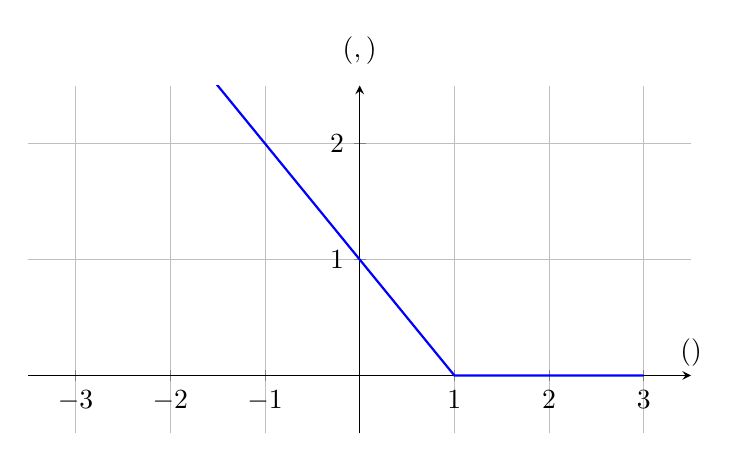
\begin{tikzpicture}
    \begin{axis}[
        axis lines=middle,
        xlabel={$\truelabel\hypothesis(\featurevec)$},
        ylabel={$\lossfunc{(\featurevec,\truelabel)}{\hypothesis}$},
 	xlabel style={at={(axis description cs:1.,0.3)}, anchor=north},  % Adjusted to be relative to axis end
        ylabel style={at={(axis description cs:0.5,1.1)}, anchor=center}, % Corrected to vertical position, rotated for readability
        xmin=-3.5, xmax=3.5,
        ymin=-0.5, ymax=2.5,
        xtick={-3, -2, -1, 0, 1, 2, 3},
        ytick={0, 1, 2},
        domain=-3:3,
        samples=100,
        width=10cm, height=6cm,
        grid=both,
        major grid style={line width=.2pt, draw=gray!50},
        minor grid style={line width=.1pt, draw=gray!20},
        legend pos=south west % Positions legend at the bottom left
    ]
        \addplot[blue, thick] {max(0, 1-x)};
     %   \addlegendentry{$\max(0, 1-x)$}
    \end{axis}
\end{tikzpicture}
	%	\end{figure} 
		\end{center}
	    Una variante regularizada de la \gls{loss} de hinge es utilizada por las \gls{svm} \cite{LampertNowKernel}. 	    
		},first={pérdida de hinge},text={pérdida de hinge}}

\newglossaryentry{iidasspt}{name={suposición de independencia e idéntica distribución (suposición i.i.d.)}, description={La suposición \gls{iid} 
		\index{suposición de independencia e idéntica distribución (suposición i.i.d.)} interpreta los \gls{datapoint}s de un\gls{dataset} como las 
		\gls{realization}s de \gls{rv}s \gls{iid}.},first={suposición de independencia e idéntica distribución (suposición i.i.d.)},text={suposición i.i.d.} }

\newglossaryentry{hypospace}{name={espacio de hipótesis}, description={Cada\index{espacio de hipótesis} 
		método práctico de\gls{ml} utiliza un espacio de \gls{hypothesis} (o \gls{model}) $\hypospace$. El espacio de \gls{hypothesis}  
		de un método de \gls{ml} es un subconjunto de todos los posibles mapeos del \gls{featurespace} al \gls{labelspace}. 
		La elección del diseño del espacio de \gls{hypothesis} debe considerar los recursos computacionales disponibles y 
		los \gls{statasp}. Si la infraestructura computacional permite operaciones matriciales eficientes y existe
		una relación (aproximadamente) lineal entre un conjunto de \gls{feature}s y una \gls{label}, una elección útil para el 
		espacio de \gls{hypothesis} podria ser el \gls{linmodel}.},first={espacio de hipótesis},text={espacio de hipótesis} }
	
\newglossaryentry{model}{name={modelo}, description={En\index{modelo} el contexto de métodos de \gls{ml}, 
		el término modelo típicamente se refiere a el \gls{hypospace} empleado por un método de
		\gls{ml} \cite{ShalevMLBook,MLBasics}.},first={modelo},text={modelo} }

\newglossaryentry{modelparams}{name={model parameters}, 
	description={\Gls{model} \gls{parameters}\index{model parameters} are quantities that 
	are used to select a specific \gls{hypothesis} map from a \gls{model}. 
	We can think of a list of \gls{model} \gls{parameters} as a unique identifier for a \gls{hypothesis} 
	map, similar to how a social security number identifies a person in Finland.},
	first={model parameters},text={model parameters} }

\newglossaryentry{ai}{name={artificial intelligence (AI)}, description={
		AI\index{artificial intelligence (AI)} refers to systems that behave rationally in the sense of 
		maximizing a long-term \gls{reward}. The \gls{ml}-based approach to AI is to train a \gls{model} for  
		predicting optimal actions. These predictions are computed from observations about the state of the 
		environment. The choice of \gls{lossfunc} sets AI applications apart from more basic \gls{ml} applications. 
		AI systems rarely have access to a labeled \gls{trainset} that allows the average \gls{loss} to be measured for any possible choice of \gls{modelparams}. 
		Instead, AI systems use observed \gls{reward} signals to obtain a (point-wise) estimate for the 
		\gls{loss} incurred by the current choice of \gls{modelparams}.},first={AI},text={AI} }

\newglossaryentry{reward}{name={reward}, description={A reward refers to some\index{reward} observed 
		(or measured) quantity that allows us to estimate the \gls{loss} incurred by the \gls{prediction} 
		(or decision) of a \gls{hypothesis} $\hypothesis(\featurevec)$. For example, in an 
		\gls{ml} application to self-driving vehicles, $\hypothesis(\featurevec)$ could represent 
		the current steering direction of a vehicle. We could construct a reward from the 
		measurements of a collision sensor that indicate if the vehicle is moving towards 
		an obstacle. We define a low reward for the steering direction 
	$\hypothesis(\featurevec)$ if the vehicle moves dangerously towards an obstacle.},
	first={reward}, text={reward}} 

\newglossaryentry{hardclustering}{name={hard clustering}, description={Hard \gls{clustering}\index{hard clustering} 
		refers to the task of partitioning a given set of \gls{datapoint}s into (a few) non-overlapping \gls{cluster}s. 
		The most widely used hard \gls{clustering} method is \gls{kmeans}.},first={hard clustering},text={hard clustering} }
	
\newglossaryentry{softclustering}{name={soft clustering}, description={Soft \gls{clustering}\index{soft clustering} 
		refers to the task of partitioning a given set of \gls{datapoint}s into (a few) overlapping \gls{cluster}s. 
		Each \gls{datapoint} is assigned to several different \gls{cluster}s with varying degrees of belonging. Soft \gls{clustering} 
		methods determine the \gls{dob} (or soft \gls{cluster} assignment) for each \gls{datapoint} and each \gls{cluster}.
		A principled approach to soft \gls{clustering} is by interpreting \gls{datapoint}s as \gls{iid} \gls{realization}s 
		of a \gls{gmm}. We then obtain a natural choice for the \gls{dob} as the conditional 
		\gls{probability} of a \gls{datapoint} belonging to a specific mixture component.},first={soft clustering},text={soft clustering} }
	
\newglossaryentry{clustering}{name={clustering}, description={Clustering\index{clustering} methods decompose a given 
		set of \gls{datapoint}s into a few subsets, which are referred to as \gls{cluster}s. 
		Each \gls{cluster} consists of \gls{datapoint}s that are more similar to each 
		other than to \gls{datapoint}s outside the \gls{cluster}. Different clustering methods 
		use different measures for the similarity between \gls{datapoint}s and different 
		forms of \gls{cluster} representations. The clustering method \gls{kmeans} uses the 
		average \gls{feature} vector (cluster \gls{mean}) of a \gls{cluster} as its representative. 
		A popular \gls{softclustering} method based on \gls{gmm} represents 
		a \gls{cluster} by a \gls{mvndist}.},first={clustering},text={clustering} }
	
\newglossaryentry{cluster}{name={cluster}, description={A\index{cluster} cluster is a subset of 
		\gls{datapoint}s that are more similar to each other than to the \gls{datapoint}s outside the cluster. 
		The quantitative measure of similarity between \gls{datapoint}s is a design choice. If \gls{datapoint}s 
		are characterized by Euclidean \gls{featurevec}s $\featurevec \in \mathbb{R}^{\nrfeatures}$, 
		we can define the similarity between two \gls{datapoint}s via the Euclidean distance between 
		their \gls{featurevec}s.},first={cluster},text={cluster} }

%\newglossaryentry{softclustering}{name={soft clustering}, description={Soft clustering methods determine, for each \gls{datapoint} within a dataset, 
%		a soft cluster assignment or the degree of belonging to a particular cluster.},first={soft clustering},text={soft clustering} }


\newglossaryentry{huberloss}{name={Huber loss}, description={The\index{Huber loss} 
		Huber \gls{loss} unifies the \gls{sqerrloss} and the \gls{abserr}.},first={Huber loss},text={Huber loss} }

\newglossaryentry{svm}{name={support vector machine (SVM)}, description={The\index{support vector machine (SVM)} 
		SVM is a binary \gls{classification} method that 
		learns a linear \gls{hypothesis} map. Thus, like \gls{linreg} and \gls{logreg}, 
		it is also an instance of \gls{erm} for the \gls{linmodel}. However, the 
		SVM uses a different \gls{lossfunc} from the one used in those methods. As illustrated in 
		Figure \ref{fig_svm_gls_dict}, it aims to maximally separate \gls{datapoint}s from 
		the two different classes in the \gls{featurespace} (i.e., \gls{maximum} margin principle). 
		Maximizing this separation is equivalent to minimizing a regularized 
		variant of the \gls{hingeloss} \eqref{equ_hinge_loss_gls_dict} \cite{LampertNowKernel,Cristianini_Shawe-Taylor_2000,BishopBook}.
		\begin{figure}[H]
			\begin{center}
				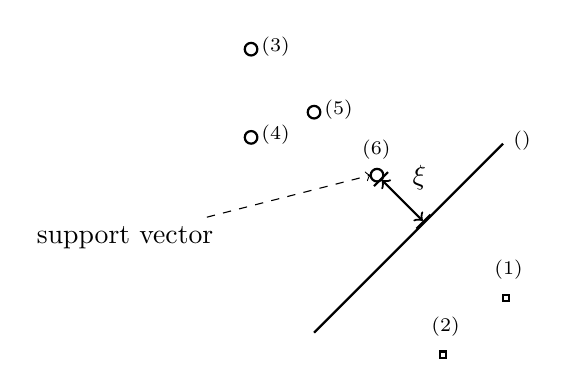
\begin{tikzpicture}[auto,scale=0.8]
					%\draw [thick] (0,-3) rectangle (4,4) node [anchor=east,above] {$\featurespace$} ;
					\draw [thick] (1,2) circle (0.1cm)node[anchor=west] {\hspace*{0mm}$\featurevec^{(5)}$};
					\draw [thick] (0,1.6) circle (0.1cm)node[anchor=west] {\hspace*{0mm}$\featurevec^{(4)}$};
					\draw [thick] (0,3) circle (0.1cm)node[anchor=west] {\hspace*{0mm}$\featurevec^{(3)}$};
					\draw [thick] (2,1) circle (0.1cm)node[anchor=east,above] {\hspace*{0mm}$\featurevec^{(6)}$};
					\node[] (B) at (-2,0) {support vector};
					\draw[->,dashed] (B) to (1.9,1) ; 
					\draw [|<->|,thick] (2.05,0.95)  -- (2.75,0.25)node[pos=0.5] {$\xi$} ; 
					\draw [thick] (1,-1.5) -- (4,1.5) node [right] {$\hypothesis^{(\weights)}$} ; 
					\draw [thick] (3,-1.9) rectangle ++(0.1cm,0.1cm) node[anchor=west,above]  {\hspace*{0mm}$\featurevec^{(2)}$};
					\draw [thick] (4,.-1) rectangle ++(0.1cm,0.1cm) node[anchor=west,above] {\hspace*{0mm}$\featurevec^{(1)}$};
				\end{tikzpicture}
				\caption{The \gls{svm} learns a \gls{hypothesis} (or \gls{classifier}) $\hypothesis^{(\weights)}$ with 
					minimal average soft-margin \gls{hingeloss}. Minimizing this \gls{loss} is equivalent 
					to maximizing the margin $\xi$ between the \gls{decisionboundary} of $\hypothesis^{(\weights)}$ 
					and each class of the \gls{trainset}.}
				\label{fig_svm_gls_dict}
			\end{center}
		\end{figure}
		The above basic variant of SVM is only useful if the \gls{datapoint}s from different categories can be  
		(approximately) linearly separated. For an \gls{ml} application where the categories are not 
		%linearly separable based on the the original (raw) \gls{feature}s it is possible to apply the SVM 
		%to transformed \gls{feature}s. These transformed \gls{feature}s can be obtained by applying a \gls{featuremap} 
		derived from a \gls{kernel}.
},first={support vector machine (SVM)},text={SVM} }

\newglossaryentry{eigenvalue}{name={eigenvalue}, description={We\index{eigenvalue} refer to a 
		number $\lambda \in \mathbb{R}$ as an eigenvalue of a square matrix $\mathbf{A} \in \mathbb{R}^{\featuredim \times \featuredim}$ 
		if there is a non-zero vector $\vx \in \mathbb{R}^{\featuredim} \setminus \{ \mathbf{0} \}$ such that $\mathbf{A} \vx = \lambda \vx$. },first={eigenvalue},text={eigenvalue} }
	
\newglossaryentry{eigenvector}{name={eigenvector}, description={An\index{eigenvector} 
		eigenvector of a matrix $\mathbf{A} \in \mathbb{R}^{\featuredim \times \featuredim}$ 
		is a non-zero vector $\vx \in \mathbb{R}^{\featuredim} \setminus \{ \mathbf{0} \}$ 
		such that $\mathbf{A} \vx = \lambda \vx$ with some \gls{eigenvalue} $\lambda$.},first={eigenvector},text={eigenvector} }

\newglossaryentry{evd}{name={eigenvalue decomposition (EVD)}, 
	description={The\index{eigenvalue decomposition (EVD)} \gls{eigenvalue} 
		decomposition for a square matrix $\mA \in \mathbb{R}^{\dimlocalmodel \times \dimlocalmodel}$ 
		is a factorization of the form 
		$$\mA = \mathbf{V} {\bm \Lambda} \mathbf{V}^{-1}.$$ 
		The columns of the matrix $\mV = \big( \vv^{(1)},\ldots,\vv^{(\dimlocalmodel)} \big)$ are the 
		\gls{eigenvector}s of the matrix $\mV$. The diagonal matrix 
		${\bm \Lambda} = {\rm diag} \big\{ \eigval{1},\ldots,\eigval{\dimlocalmodel} \big\}$ 
		contains the \gls{eigenvalue}s $\eigval{\featureidx}$ corresponding to the \gls{eigenvector}s $\vv^{(\featureidx)}$. 
		Note that the above decomposition exists only if the matrix $\mA$ is diagonalizable.},first={eigenvalue decomposition (EVD)},text={EVD} }

\newglossaryentry{svd}{name={singular value decomposition (SVD)}, 
  	description={The\index{singular value decomposition (SVD)} SVD  
  		for a matrix $\mA \in \mathbb{R}^{\samplesize \times \dimlocalmodel}$ 
		is a factorization of the form 
		$$\mA = \mathbf{V} {\bm \Lambda} \mathbf{U}^{T},$$ 
		with orthonormal matrices $\mV \in \mathbb{R}^{\samplesize \times \samplesize}$ 
		and $\mU \in \mathbb{R}^{\dimlocalmodel \times \dimlocalmodel}$ \cite{GolubVanLoanBook}. 
		The matrix ${\bm \Lambda} \in \mathbb{R}^{\samplesize \times \dimlocalmodel}$ is 
		only non-zero along the main diagonal, whose entries $\Lambda_{\featureidx,\featureidx}$ 
		are non-negative and referred to as singular values.
	},first={singular value decomposition (SVD)},text={SVD} }


\newglossaryentry{tv}{name={total variation}, description={See \gls{gtv}\index{total variation}.},
	first={total variation},text={total variation} }

 \newglossaryentry{cvxclustering}{name={convex clustering}, 
 	description={Consider\index{convex clustering} a \gls{dataset} 
 	$\featurevec^{(1)},\ldots,\featurevec^{(\samplesize)} \in \mathbb{R}^{\nrfeatures}$. 
 	\Gls{convex} \gls{clustering} learns vectors $\weights^{(1)},\ldots,\weights^{(\samplesize)}$ by 
 	minimizing 
 	$$ \sum_{\sampleidx=1}^{\samplesize} \normgeneric{\featurevec^{(\sampleidx)} - \weights^{(\sampleidx)}}{2}^2 + 
 	\regparam \sum_{\nodeidx,\nodeidx' \in \nodes} \normgeneric{\weights^{(\nodeidx)} - \weights^{(\nodeidx')}}{p}.$$ 
	Here, $ \normgeneric{\vu}{p} \defeq \big( \sum_{\featureidx=1}^{\dimlocalmodel} |u_{\featureidx}|^{p} \big)^{1/p}$ 
	denotes the $p$-\gls{norm} (for $p\geq1$).  
	It turns out that many of the optimal vectors $\widehat{\weights}^{(1)},\ldots,\widehat{\weights}^{(\samplesize)}$ 
	coincide. A \gls{cluster} then consists of those \gls{datapoint}s $\sampleidx \in \{1,\ldots,\samplesize\}$ 
	with identical $\widehat{\weights}^{(\sampleidx)}$ \cite{JMLR:v22:18-694,Pelckmans2005}. 
 	  },
 		first={convex clustering},text={convex clustering} }


\newglossaryentry{gdmethods}{name={gradient-based methods}, 
	description={\Gls{gradient}-based\index{gradient-based methods} 
		methods are iterative techniques for finding the \gls{minimum} (or \gls{maximum}) 
		of a \gls{differentiable} \gls{objfunc} of the \gls{modelparams}. These 
		methods construct a sequence of approximations to an optimal choice for 
		\gls{modelparams} that results in a \gls{minimum} (or \gls{maximum}) value of the \gls{objfunc}. 
		As their name indicates, \gls{gradient}-based methods use the \gls{gradient}s of the \gls{objfunc} 
		evaluated during previous iterations to construct new, (hopefully) improved \gls{modelparams}. 
		One important example of a \gls{gradient}-based method is \gls{gd}.},
		first={gradient-based methods},text={gradient-based methods} }

\newglossaryentry{sgd}{name={subgradient descent}, description={\Gls{subgradient}\index{subgradient descent} 
		descent is a \gls{generalization} of \gls{gd} that does not require differentiability of the 
		function to be minimized. This \gls{generalization} is obtained by replacing the concept 
		of a \gls{gradient} with that of a \gls{subgradient}. Similar to \gls{gradient}s, also \gls{subgradient}s 
		allow us to construct local approximations of an \gls{objfunc}. The \gls{objfunc} 
		might be the \gls{emprisk} $\emperror\big( \hypothesis^{(\weights)} \big| \dataset \big)$ viewed 
		as a function of the \gls{modelparams} $\weights$ that select a \gls{hypothesis} $\hypothesis^{(\weights)} \in \hypospace$.},first={subgradient descent},text={subgradient descent} }
	
\newglossaryentry{stochGD}{name={stochastic gradient descent (SGD)}, description={Stochastic\index{stochastic gradient descent (SGD)} 
		\gls{gd} is obtained from \gls{gd} by replacing the \gls{gradient} of the \gls{objfunc} 
		with a stochastic approximation. A main application of stochastic \gls{gd} 
		is to train a parametrized \gls{model} via \gls{erm} on a \gls{trainset} $\dataset$ that 
		is either very large or not readily available (e.g., when \gls{datapoint}s are stored 
		in a database distributed all over the planet). To evaluate the \gls{gradient} of the 
		\gls{emprisk} (as a function of the \gls{modelparams} $\weights$), 
		we need to compute a sum $\sum_{\sampleidx=1}^{\samplesize} \nabla_{\weights} \lossfunc{\datapoint^{(\sampleidx)}}{\weights}$  
		over all \gls{datapoint}s in the \gls{trainset}. We obtain a stochastic 
		approximation to the \gls{gradient} by replacing the sum $\sum_{\sampleidx=1}^{\samplesize} \nabla_{\weights} \lossfunc{\datapoint^{(\sampleidx)}}{\weights}$ 
		with a sum $\sum_{\sampleidx \in \batch} \nabla_{\weights} \lossfunc{\datapoint^{(\sampleidx)}}{\weights}$ 
		over a randomly chosen subset $\batch \subseteq \{1,\ldots,\samplesize\}$ (see Figure \ref{fig_sgd_approx_dict}). 
		We often refer to these randomly chosen \gls{datapoint}s as a \gls{batch}. 
		The \gls{batch} size $|\batch|$ is an important parameter of stochastic \gls{gd}. 
		Stochastic \gls{gd} with $|\batch|> 1$ is referred to as mini-\gls{batch} stochastic \gls{gd} \cite{Bottou99}. 		
		\begin{figure}[H]
			\centering
			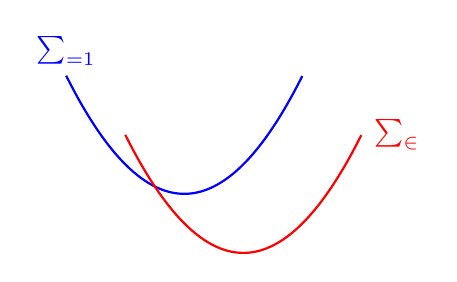
\begin{tikzpicture}[scale=1.5, >=stealth]
% Axes
				%\draw[->] (-1, 0) -- (4, 0) node[right] {$w$};
				%\draw[->] (0, -0.5) -- (0, 4) node[above] {};
% First quadratic function: f(w)
				\draw[thick, blue, domain=0.5:2.5, samples=100] plot (\x, {(\x-1.5)^2 + 1});
				\node[blue,above] at (0.5, 2) {$\sum_{\sampleidx=1}^{\samplesize}$};
% Second quadratic function: f'(w)
				\draw[thick, red, domain=1:3, samples=100] plot (\x, {(\x-2)^2 + 0.5});
				\node[red] at (3.3, 1.5) {$\sum_{\sampleidx \in \batch}$};
% Labels
			\end{tikzpicture}
		\caption{Stochastic \gls{gd} for \gls{erm} approximates the \gls{gradient} 
		$\sum_{\sampleidx=1}^{\samplesize} \nabla_{\weights} \lossfunc{\datapoint^{(\sampleidx)}}{\weights}$ 
		by replacing the 
		sum over all \gls{datapoint}s in the \gls{trainset} (indexed by $\sampleidx=1,\ldots,\samplesize$) 
		with a sum over a randomly chosen subset $\batch \subseteq \{1,\ldots,\samplesize\}$.\label{fig_sgd_approx_dict}}
		\end{figure}
},first={stochastic gradient descent (SGD)},text={SGD} }


\newglossaryentry{onlineGD}{name={online gradient descent (online GD)}, description={
Consider \index{online gradient descent (online GD)} an \gls{ml} method that learns \gls{modelparams} 
$\weights$ from some \gls{paramspace} $\paramspace \subseteq \mathbb{R}^{\dimlocalmodel}$. 
The learning process uses \gls{datapoint}s $\datapoint^{(\timeidx)}$ that arrive at consecutive time-instants $\timeidx=1,2,\ldots$. 
Let us interpret the \gls{datapoint}s $\datapoint^{(\timeidx)}$ as \gls{iid} copies 
of an \gls{rv} $\datapoint$. The \gls{risk} $\expect\{ \lossfunc{\datapoint}{\weights} \}$ of a 
\gls{hypothesis} $\hypothesis^{(\weights)}$ can then (under mild conditions) be obtained as the limit 
$\lim_{T\rightarrow \infty} (1/T)\sum_{\timeidx=1}^{T} \lossfunc{\datapoint^{(\timeidx)}}{\weights}$. 
We might use this limit as the \gls{objfunc} for learning the \gls{modelparams} $\weights$. 
Unfortunately, this limit can only be evaluated if we wait infinitely long in order to collect all \gls{datapoint}s. 
Some \gls{ml} applications require methods that learn online: as soon as a new \gls{datapoint} $\datapoint^{(\timeidx)}$ 
arrives at time $\timeidx$, we update the current \gls{modelparams} $\weights^{(\timeidx)}$. Note that 
the new \gls{datapoint} $\datapoint^{(\timeidx)}$ contributes the component $\lossfunc{\datapoint^{(\timeidx)}}{\weights}$ 
to the \gls{risk}. As its name suggests, online \gls{gd} updates $\weights^{(\timeidx)}$ via a (projected) \gls{gradstep}
\begin{equation} 
\label{equ_def_ogd_dict}
 \weights^{(\timeidx+1)} \defeq \projection{\paramspace}{\weights^{(\timeidx)} - \lrate_{\timeidx} \nabla_{\weights} \lossfunc{\datapoint^{(\timeidx)}}{\weights}}. 
\end{equation} 
Note that \eqref{equ_def_ogd_dict} is a \gls{gradstep} for the current component $\lossfunc{\datapoint^{(\timeidx)}}{\cdot}$ 
of the \gls{risk}. The update \eqref{equ_def_ogd_dict} ignores all the previous components $\lossfunc{\datapoint^{(\timeidx')}}{\cdot}$, 
for $\timeidx' < \timeidx$. It might therefore happen that, compared to $\weights^{(\timeidx)}$, the updated \gls{modelparams} 
$\weights^{(\timeidx+1)}$ increase the retrospective average \gls{loss} $\sum_{\timeidx'=1}^{\timeidx-1} \lossfunc{\datapoint^{(\timeidx')}}{\cdot}$. 
However, for a suitably chosen \gls{learnrate} $\lrate_{\timeidx}$, online \gls{gd} can be shown 
to be optimal in practically relevant settings. By optimal, we mean that the \gls{modelparams} 
$\weights^{(T+1)}$ delivered by online \gls{gd} after observing $T$ \gls{datapoint}s $\datapoint^{(1)},\ldots, \datapoint^{(T)}$ 
are at least as good as those delivered by any other learning method \cite{HazanOCO,GDOptimalRakhlin2012}. 
\begin{figure}[H]
	\begin{center}
\begin{tikzpicture}[x=1.5cm,scale=1.5, every node/.style={font=\footnotesize}]
	% Axes
	\draw[->] (0.5, 0) -- (5.5, 0) node[below] {};
	%\draw[->] (0, -0.5) -- (0, 3) node[left] {Value};
	% Labels for time steps
	\foreach \x in {1, 2, 3, 4, 5} {
		\draw (\x, 0.1) -- (\x, -0.1) node[below] {$t=\x$};
	}
	% Data points (black circles)
	\foreach \x/\y in {1/2.5, 2/1.8, 3/2.3, 4/1.5, 5/2.0} {
		\fill[black] (\x, \y) circle (2pt) node[above right] {$\datapoint^{(\x)}$};
	}
	% Model parameters (blue circles)
	\foreach \x/\y in {1/1.0, 2/1.6, 3/1.8, 4/2.2, 5/1.9} {
		\fill[blue] (\x, \y) circle (2pt) node[below left] {$\weights^{(\x)}$};
	}
	% Connecting lines (model tracking data)
	\foreach \x/\y/\z in {1/2.5/1.0, 2/1.8/1.6, 3/2.3/2.0, 4/1.5/1.8, 5/2.0/1.9} {
		\draw[dashed, gray] (\x, \y) -- (\x, \z);
	}
	% Legend
	% \node[draw, fill=white] at (4.5, 2.7) {
	% 	\begin{tabular}{@{}ll@{}}
	% 		\textcolor{black}{$\bullet$} & Data Point ($d_t$) \\
	% 		\textcolor{blue}{$\bullet$} & Model Parameter ($\theta_t$) \\
	% 		\textcolor{gray}{\rule{1cm}{0.5pt}} & Gradient Update
	% 	\end{tabular}
	%};
	\end{tikzpicture}
\end{center} 
\caption{An instance of online \gls{gd} that updates the \gls{modelparams} $\weights^{(\timeidx)}$ 
using the \gls{datapoint} $\datapoint^{(\timeidx)} = \feature^{(\timeidx)}$ arriving at time $\timeidx$. 
This instance uses the \gls{sqerrloss} $\lossfunc{\datapoint^{(\timeidx)}}{\weight} = (\feature^{(\timeidx)} - \weight)^{2}$.
}
\end{figure}},
first={online gradient descent (online GD)},text={online GD}}

\newglossaryentry{pca}{name={principal component analysis (PCA)}, description={PCA\index{principal component analysis (PCA)} 
		determines a linear \gls{featuremap} such that the new \gls{feature}s 
		allow us to reconstruct the original \gls{feature}s with the \gls{minimum} reconstruction error \cite{MLBasics}.},first={principal component analysis (PCA)},text={PCA} }
	
\newglossaryentry{loss}{name={loss}, description={\gls{ml}\index{loss} methods use a 
		\gls{lossfunc} $\lossfunc{\datapoint}{\hypothesis}$ to measure the error incurred 
		by applying a specific \gls{hypothesis} to a specific \gls{datapoint}. With a
		slight abuse of notation, we use the term loss for both the \gls{lossfunc} $\loss$ 
		itself and the specific value $\lossfunc{\datapoint}{\hypothesis}$, for a \gls{datapoint} $\datapoint$ 
		and \gls{hypothesis} $\hypothesis$.},first={loss},text={loss} }

\newglossaryentry{lossfunc}{name={loss function}, description={A\index{loss function} \gls{loss} function is a map 
		$$\lossfun: \featurespace \times \labelspace \times \hypospace \rightarrow \mathbb{R}_{+}: \big( \big(\featurevec,\truelabel\big),
		 \hypothesis\big) \mapsto  \lossfunc{(\featurevec,\truelabel)}{\hypothesis}.$$
		It assigns a non-negative real number (i.e., the \gls{loss}) $\lossfunc{(\featurevec,\truelabel)}{\hypothesis}$
		to a pair that consists of a \gls{datapoint}, with \gls{feature}s $\featurevec$ 
		and \gls{label} $\truelabel$, and a \gls{hypothesis} $\hypothesis \in \hypospace$. The 
		value $\lossfunc{(\featurevec,\truelabel)}{\hypothesis}$ quantifies the discrepancy 
		between the true \gls{label} $\truelabel$ and the \gls{prediction} $\hypothesis(\featurevec)$. 
		Lower (closer to zero) values $\lossfunc{(\featurevec,\truelabel)}{\hypothesis}$ indicate a smaller 
		discrepancy between \gls{prediction} $\hypothesis(\featurevec)$ and \gls{label} $\truelabel$. 
		Figure \ref{fig_loss_function_gls_dict} depicts a \gls{loss} function for a given \gls{datapoint}, 
		with \gls{feature}s $\featurevec$ and \gls{label} $\truelabel$, as a function of the \gls{hypothesis} $\hypothesis \in \hypospace$. 
		\begin{figure}[H]
			\begin{center}
				\begin{tikzpicture}[scale = 0.7]
					\begin{axis}
						[%grid, 
						axis x line=center,
						axis y line=center,
						%	xtick={-2,-1,...,2},
						%	ytick={0,1,...,2},
						xlabel={},
						%	ylabel={\hspace*{3mm} loss $\lossfun$},
						xlabel style={below right},
						ylabel style={above right},
						xtick=\empty,
						ytick=\empty,
						xmin=-4,
						xscale = 1.4, 
						xmax=4,
						ymin=-0.5,
						ymax=2.5
						]
						\addplot [smooth, ultra thick] table [x=a, y=b, col sep=comma] {../../assets/logloss.csv};    
					\end{axis}
					\node [above] at (1,5) {$\lossfunc{(\featurevec,\truelabel)}{\hypothesis}$};
					\node [above] at (10,1) {\gls{hypothesis} $\hypothesis$};
						\node [right] at (4,6) {\gls{loss}};
				\end{tikzpicture}
			\end{center}
			\vspace*{-7mm}
			\caption{Some \gls{loss} function $\lossfunc{(\featurevec,\truelabel)}{\hypothesis}$ for a fixed \gls{datapoint}, with 
				\gls{featurevec} $\featurevec$ and \gls{label} $\truelabel$, and a varying \gls{hypothesis} $\hypothesis$. 
				\gls{ml} methods try to find (or learn) a \gls{hypothesis} that incurs minimal \gls{loss}.}
			\label{fig_loss_function_gls_dict}
	\end{figure}
 },first={loss function},text={loss function} }

\newglossaryentry{decisiontree}{name={decision tree}, description={A\index{decision tree} 
		decision tree is a flow-chart-like representation of a \gls{hypothesis} map $\hypothesis$. 
		More formally, a decision tree is a directed \gls{graph} containing a root node that reads 
		in the \gls{featurevec} $\featurevec$ of a \gls{datapoint}. The root node then forwards 
		the \gls{datapoint} to one of its children nodes based on some elementary test on the \gls{feature}s $\featurevec$. 
		If the receiving child node is not a leaf node, i.e., it has itself children nodes, 
	  it represents another test. Based on the test result, the \gls{datapoint} is forwarded 
	   to one of its descendants. This testing and forwarding of the \gls{datapoint} is continued 
	  until the \gls{datapoint} ends up in a leaf node (having no children nodes). 
\begin{figure}[H]
\begin{minipage}{.45\textwidth}
	\scalebox{1}{
\begin{tikzpicture}
%	% Root node
	\node[fill=black, circle, inner sep=2pt, label=above:{$\| \featurevec-\mathbf{u} \| \leq \varepsilon$?}] (A) {};	
%	% Left child (h1)
	\node[fill=black, circle, inner sep=2pt, below left=1.5cm and 1cm of A, label=left:{$\hypothesis(\featurevec) = \predictedlabel_1$}] (B) {};
	% Right child (next question)
	\node[fill=black, circle, inner sep=2pt, below right=1.5cm and 1cm of A, label=right:{$\| \featurevec - \mathbf{v} \| \leq \varepsilon$?}] (C) {};
%	% Left child of C (h2)
	\node[fill=black, circle, inner sep=2pt, below left=1.5cm and 1cm of C, label=left:{$\hypothesis(\featurevec) = \predictedlabel_2$}] (D) {};
	% Right child of C (h3)
	\node[fill=black, circle, inner sep=2pt, below right=1.5cm and 1cm of C, label=right:{$\hypothesis(\featurevec) =\predictedlabel_3$}] (E) {};
%	% Arrows
	\draw[line width=1.5pt, ->] (A) -- (B) node[midway, left] {no};
	\draw[line width=1.5pt, ->] (A) -- (C) node[midway, right] {yes};
	\draw[line width=1.5pt, ->] (C) -- (D) node[midway, left] {no};
	\draw[line width=1.5pt, ->] (C) -- (E) node[midway, right] {yes};
\end{tikzpicture}
	}
\end{minipage}	
\hspace*{15mm}
\begin{minipage}{.45\textwidth}
	\hspace*{15mm}
	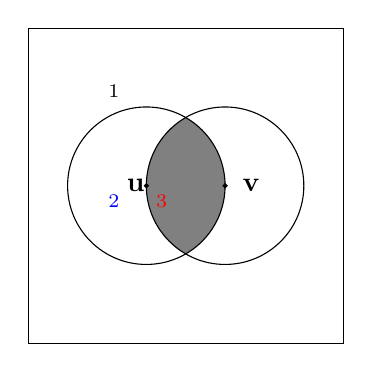
\begin{tikzpicture}
		\draw (-2,2) rectangle (2,-2);
		\begin{scope}
			\clip (-0.5,0) circle (1cm);
			\clip (0.5,0) circle (1cm);
			\fill[color=gray] (-2,1.5) rectangle (2,-1.5);
		\end{scope}
		\draw (-0.5,0) circle (1cm);
		\draw (0.5,0) circle (1cm);
		\draw[fill] (-0.5,0) circle [radius=0.025];
		\node [below right, red] at (-0.5,0) {$\predictedlabel_{3}$};
		\node [below left, blue] at (-0.7,0) {$\predictedlabel_{2}$};
		\node [above left] at (-0.7,1) {$\predictedlabel_{1}$};
		\node [left] at (-0.4,0) {$\mathbf{u}$};
		\draw[fill] (0.5,0) circle [radius=0.025];
		\node [right] at (0.6,0) {$\mathbf{v}$};
	\end{tikzpicture}
\end{minipage}
	\caption{Left: A decision tree is a flow-chart-like representation of a piece-wise constant \gls{hypothesis} $\hypothesis: \featurespace \rightarrow \mathbb{R}$.  Each piece is a \gls{decisionregion} $\decreg{\predictedlabel} \defeq \big\{ \featurevec \in  \featurespace: \hypothesis(\featurevec) = \predictedlabel \big\}$. 
		The depicted decision tree can be applied to numeric \gls{featurevec}s, i.e., $\featurespace \subseteq \mathbb{R}^{\dimlocalmodel}$. It is  parametrized by the threshold $\varepsilon>0$ and the vectors $\vu, \vv \in \mathbb{R}^{\dimlocalmodel}$. 
		Right: A decision tree partitions  
		the \gls{featurespace} $\featurespace$ into \gls{decisionregion}s. Each \gls{decisionregion}  
		$\decreg{\hat{\truelabel}} \!\subseteq\!\featurespace$ corresponds to a specific leaf node in the decision tree.}
	\label{fig_decision_tree}
\end{figure} 
	  }
	  ,first={decision tree},text={decision tree} }

%\newglossaryentry{API} 
%{
%	name={application programming interface (API)},
%	description={An\index{application programming interface} application programming 
%		interface (API) is a precise specification of the services and resources 
%		offered by software or hardware implementing that API.},
%	first={application programming interface (API)},
%	text={API}
%}


\newglossaryentry{API} 
{name={application programming interface (API)},
		description={
			An \index{application programming interface (API)} API is a formal mechanism for enabling 
			software components to interact in a structured manner \cite{RestfulBook2013}. In the 
			context of \gls{ml}, APIs are frequently used to make a trained \gls{ml} \gls{model} 
			accessible to different types of users. These users, which can be other computers 
			or humans, can request a \gls{prediction} for the \gls{label} of a \gls{datapoint} by 
			providing its \gls{feature}s. The internal structure of the \gls{ml} 
			\gls{model} remains hidden from the user. For instance, consider a trained \gls{ml} \gls{model}  
			$\widehat{\hypothesis}(\feature) \defeq  2 \feature+1$. An API enables a user to 
			submit the \gls{feature} value $\feature=3$ and obtain the response $\widehat{\hypothesis}(3)=7$ 
			without knowledge of the detailed structure of the \gls{ml} \gls{model} or its training. 
			In practice, the \gls{ml} \gls{model} is typically hosted on a computer (i.e., a server) connected to the internet. 
			Another computer (i.e., a client) sends the \gls{feature}s of a \gls{datapoint} to the 
			server, which then computes $\widehat{\hypothesis}(\featurevec)$ and returns the 
			result to the external system. APIs help to modularize the development of 
			\gls{ml} applications by decoupling specific tasks. For instance, one team can 
			focus on developing and training the \gls{model}, while another team handles 
			user interaction and integration of the \gls{model} into applications.
			},
		first={application programming interface (API)},
		text={API}
}


\newglossaryentry{hilbertspace}{name={Hilbert space},description={A\index{Hilbert space} 
		Hilbert space is a linear vector space equipped with an inner product between 
		pairs of vectors. One important example of a Hilbert space is the \gls{euclidspace} 
		$\mathbb{R}^{\featuredim}$, for some dimension $\featuredim$, which consists of 
		Euclidean vectors $\vu = \big(u_{1},\ldots,u_{\featurelen}\big)^{T}$ along with the inner 
		product $\vu^{T} \vv$.},first={Hilbert space},text={Hilbert space}}



\newglossaryentry{sample}{name={sample},description={A\index{sample} 
		finite sequence (or list) of \gls{datapoint}s $\datapoint^{(1)},\ldots,\datapoint^{(m)}$ that 
		is obtained or interpreted as the \gls{realization} of $\samplesize$ \gls{iid} \gls{rv}s 
		with a common \gls{probdist} $p(\datapoint)$. The length $\samplesize$ of 
		the sequence is referred to as the \gls{samplesize}.},first={sample},text={sample}}
	
\newglossaryentry{samplesize}
{name=sample size,
	description={The\index{sample size} number of individual \gls{datapoint}s 
		contained in a \gls{dataset}.},first={sample size},text={sample size}
}

\newglossaryentry{ann}{
	name={artificial neural network (ANN)},
	description={An\index{artificial neural network (ANN)} ANN 
		is a graphical (signal-flow) representation of a function that maps 
		\gls{feature}s of a \gls{datapoint} at its input to a \gls{prediction} 
		for the corresponding \gls{label} at its output. The fundamental unit of an 
		ANN is the artificial neuron, which applies an \gls{actfun} to its 
		weighted inputs. The outputs of these neurons serve as inputs for other neurons, 
		forming interconnected layers.},
	first={artificial neural network (ANN)},
	text={ANN}
}


\newglossaryentry{randomforest}
{name=random forest,
	description={A\index{random forest} random forest is a set (or ensemble) of different \gls{decisiontree}s. 
		Each of these \gls{decisiontree}s is obtained by fitting a perturbed copy of 
		the original \gls{dataset}.},first = {random forest}, text={random forest}
}

\newglossaryentry{bagging}{name={bagging},description={Bagging\index{bagging} (or bootstrap aggregation) 
		is a generic technique to improve (the robustness of) a given \gls{ml} method. The idea is to use the \gls{bootstrap} 
		to generate perturbed copies of a given \gls{dataset} and then to learn a separate \gls{hypothesis} for 
		each copy. We then predict the \gls{label} of a \gls{datapoint} by combining or aggregating the individual 
		\gls{prediction}s of each separate \gls{hypothesis}. For \gls{hypothesis} maps delivering numeric \gls{label} 
		values, this aggregation could be implemented by computing the average of individual \gls{prediction}s.},first={bootstrap aggregation (bagging)},text={bagging}}

\newglossaryentry{gd}{name={gradient descent (GD)},description={\Gls{gradient}\index{gradient descent (GD)} 
		descent is an iterative method for finding the \gls{minimum} of a \gls{differentiable} function $f(\weights)$ 
		of a vector-valued argument $\weights \in \mathbb{R}^{\featurelen}$. Consider a current guess or 
		approximation $\weights^{(\itercntr)}$ for the \gls{minimum} of the function $f(\weights)$. We would like to find a new (better) vector $\weights^{(\itercntr+1)}$ 
		that has a smaller objective value $f(\weights^{(\itercntr+1)}) < f\big(\weights^{(\itercntr)}\big)$ than 
		the current guess $\weights^{(\itercntr)}$. We can achieve this typically by using a \gls{gradstep}
		\begin{equation} 
			\label{equ_def_GD_step_dict}
			\weights^{(\itercntr\!+\!1)} = \weights^{(\itercntr)} - \lrate \nabla f(\weights^{(\itercntr)})
		\end{equation} 
		with a sufficiently small \gls{stepsize} $\lrate\!>\!0$. Figure \ref{fig_basic_GD_step_dict} illustrates the effect of 
		a single \gls{gradient} descent step \eqref{equ_def_GD_step_dict}.
		\begin{figure}[H]
			\begin{center}
				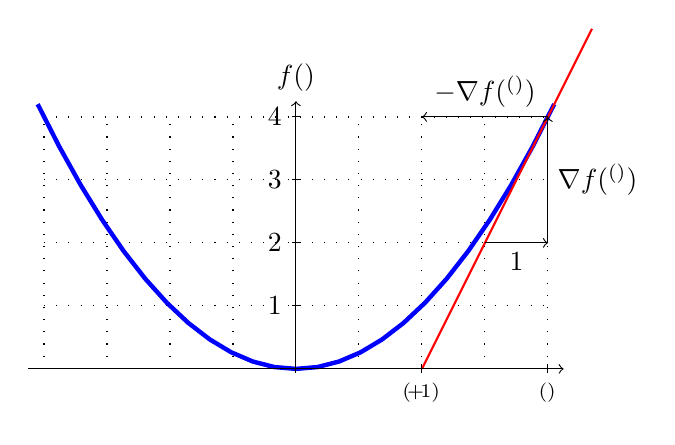
\begin{tikzpicture}[scale=0.8]
					\draw[loosely dotted] (-4,0) grid (4,4);
					\draw[blue, ultra thick, domain=-4.1:4.1] plot (\x,  {(1/4)*\x*\x});
					\draw[red, thick, domain=2:4.7] plot (\x,  {2*\x - 4});
					\draw[<-] (4,4) -- node[right] {$\nabla f(\weights^{(\itercntr)})$} (4,2);
					\draw[->] (4,4) -- node[above] {$-\lrate \nabla f(\weights^{(\itercntr)})$} (2,4);
					\draw[<-] (4,2) -- node[below] {$1$} (3,2) ;
					\draw[->] (-4.25,0) -- (4.25,0) node[right] {$\weights$};
					\draw[->] (0,-2pt) -- (0,4.25) node[above] {$f(\weights)$};
					\draw[shift={(0,0)}] (0pt,2pt) -- (0pt,-2pt) node[below] {$\overline{\weights}$};
					\draw[shift={(4,0)}] (0pt,2pt) -- (0pt,-2pt) node[below] {$\weights^{(\itercntr)}$};
					\draw[shift={(2,0)}] (0pt,2pt) -- (0pt,-2pt) node[below] {$\weights^{(\itercntr\!+\!1)}$};
					\foreach \y/\ytext in {1/1, 2/2, 3/3, 4/4}
					\draw[shift={(0,\y)}] (2pt,0pt) -- (-2pt,0pt) node[left] {$\ytext$};  
				\end{tikzpicture}
			\end{center}
			\caption{A single \gls{gradstep} \eqref{equ_def_GD_step_dict} towards the minimizer $\overline{\weights}$ of $f(\weights)$.}
			\label{fig_basic_GD_step_dict}
		\end{figure}
%		
		},first={gradient descent (GD)},text={GD}}

\newglossaryentry{abserr}{name={absolute error loss},description={
			Consider a \gls{datapoint} with \gls{feature}s $\featurevec \in \featurespace$ and numeric 
			\gls{label} $\truelabel \in \mathbb{R}$. The absolute error \gls{loss}\index{absolute error loss} 
			incurred by a \gls{hypothesis} $\hypothesis: \featurespace \rightarrow \mathbb{R}$ 
			is defined as $|\truelabel - \hypothesis(\featurevec)|$, i.e., the absolute difference between 
			the \gls{prediction} $\hypothesis(\featurevec)$ and the true \gls{label} $\truelabel$.},
	%		{\bf Example.} Imagine you are predicting the temperature for tomorrow. If the actual 
	%		temperature is 20 (measured in degree Celsius), but your model predicts 18, the absolute 
	%		error is $20−18=2$. This means your prediction was off by $2$ (degrees Celius). 
	%		The absolute error loss always gives a positive number, so it doesn't matter if the \gls{prediction} 
	%		is too high or too low - only the size of the difference matters.}
			first={absolute error loss},text={absolute error loss}}

\newglossaryentry{device}{name={device},description={
				Any\index{device} physical system that can be used to store and process \gls{data}. In the context of \gls{ml}, 
				we typically mean a computer that is able to read in \gls{datapoint}s from different 
				sources and, in turn, to train an \gls{ml} \gls{model} using these \gls{datapoint}s.},
				first={device},text={device}}

\newglossaryentry{llm}{name={large language model (LLM)},description={
	Large language \gls{model}s\index{large language model (LLM)} is an umbrella term for \gls{ml} methods 
	that process and generate human-like text. These methods typically 
	use \gls{deepnet}s with billions (or even trillions) of \gls{parameters}. 
	A widely used choice for the network architecture is referred to as 
	Transformers \cite{vaswani2017attention}. The training of large language \gls{model}s is often  
	based on the task of predicting a few words that are intentionally removed 
	from a large text corpus. Thus, we can construct \gls{labeled datapoint}s 
	simply by selecting some words of a text as \gls{label}s and the remaining 
	words as \gls{feature}s of \gls{datapoint}s. This construction requires 
	very little human supervision and allows for generating sufficiently 
	large \gls{trainset}s for large language \gls{model}s.},
					first={large language model (LLM)},text={LLM}}


\newglossaryentry{huberreg}{name={Huber regression},description={
			Huber \gls{regression}\index{Huber regression} refers to \gls{erm}-based methods 
			that use the \gls{huberloss} as a measure of the \gls{prediction} error. 
			Two important special cases of Huber \gls{regression} are \gls{ladregression} and 
			\gls{linreg}. Tuning the threshold parameter of the \gls{huberloss} allows the user
			to trade the robustness of the \gls{abserr} 
			against the computational benefits of the \gls{smooth} \gls{sqerrloss}.},
			first={Huber regression},text={Huber regression}}


\newglossaryentry{ladregression}{name={least absolute deviation regression},description={
		Least\index{least absolute deviation regression} absolute deviation regression is 
		an instance of \gls{erm} using the \gls{abserr}. It is a special case of 
		\gls{huberreg}.},
		first={least absolute deviation regression},text={least absolute deviation regression}}

%\newglossaryentry{metric}{name={metric},description={We\index{metric} sometimes use \emph{metric} to refer to 
%		a \gls{lthat is used solely 
%	    for the final performance evaluation of a learnt hypothesis. The metric is typically a \gls{lossfunc} that 
%	    has a ``natural'' interpretation (such as the \gls{zerooneloss}) but is not a good choice to guide 
%	    the learning process, e.g., via \gls{erm}. For \gls{erm}, we typically prefer \gls{lossfunc}s that depend smoothly 
%	    on the (parameters of the) hypothesis. Examples for such smooth \gls{lossfunc}s include the \gls{sqerrloss} 
%	    and the \gls{logloss} \eqref{equ_log_loss_gls}.},first={metric},text={metric}}

\newglossaryentry{bayesrisk}{name={Bayes risk},description={Consider a \gls{probmodel} with a 
joint \gls{probdist} $p(\featurevec,\truelabel)$ for the \gls{feature}s $\featurevec$ 
and \gls{label} $\truelabel$ of a \gls{datapoint}. The\index{Bayes risk} Bayes \gls{risk} 
is the \gls{minimum} possible \gls{risk} that can be achieved by any \gls{hypothesis} 
$\hypothesis: \featurespace \rightarrow \labelspace$. Any \gls{hypothesis} that achieves 
the Bayes risk is referred to as a \gls{bayesestimator} \cite{LC}.},first={Bayes risk},text={Bayes risk}}
	
\newglossaryentry{bayesestimator}{name={Bayes estimator},description={Consider\index{Bayes estimator} 
a \gls{probmodel} with a joint \gls{probdist} $p(\featurevec,\truelabel)$ for the \gls{feature}s $\featurevec$ and \gls{label} 
$\truelabel$ of a \gls{datapoint}. For a given \gls{lossfunc} $\lossfunc{\cdot}{\cdot}$, we refer to a \gls{hypothesis} 
$\hypothesis$ as a Bayes estimator if its \gls{risk} $\expect\{\lossfunc{\pair{\featurevec}{\truelabel}}{\hypothesis}\}$ is the 
\gls{minimum} \cite{LC}. Note that the property of a \gls{hypothesis} being a Bayes estimator depends on 
the underlying \gls{probdist} and the choice for the \gls{lossfunc} $\lossfunc{\cdot}{\cdot}$.},
		first={Bayes estimator},text={Bayes estimator}}


\newglossaryentry{weights}{name={weights},
	description={Consider\index{weights} a parametrized \gls{hypospace} $\hypospace$. 
		We\index{weights} use the term weights for numeric \gls{modelparams} that are 
		used to scale \gls{feature}s or their transformations in order to compute $\hypothesis^{(\weights)} \in \hypospace$. A \gls{linmodel} uses weights $\weights=\big(\weight_{1},\ldots,\weight_{\nrfeatures}\big)^{T}$ to compute 
		the linear combination $\hypothesis^{(\weights)}(\featurevec)= \weights^{T} \featurevec$. 
		Weights are also used in \gls{ann}s to form linear combinations of \gls{feature}s or the 
		outputs of neurons in hidden layers.},first={weights},text={weights}}
	
\newglossaryentry{probdist}{name={probability distribution},
	description={To\index{probability distribution} analyze \gls{ml} methods, it can be useful 
		to interpret \gls{datapoint}s as \gls{iid} \gls{realization}s of an \gls{rv}. The typical 
		properties of such \gls{datapoint}s are then governed by the \gls{probability} distribution 
		of this \gls{rv}. The \gls{probability} distribution of a binary \gls{rv} $\truelabel \in \{0,1\}$ 
		is fully specified by the probabilities $\prob{\truelabel = 0}$ and 
		$\prob{\truelabel=1}\!=\!1\!-\!\prob{\truelabel=0}$. The \gls{probability} 
		distribution of a real-valued \gls{rv} $\feature \in \mathbb{R}$ might be specified 
		by a \gls{pdf} $p(\feature)$ such that $\prob{ \feature \in [a,b] } \approx  p(a) |b-a|$. 
	    In the most general case, a \gls{probability} distribution is defined by a \gls{probability} measure \cite{GrayProbBook,BillingsleyProbMeasure}.},first={probability distribution},text={probability distribution}}
    
    
\newglossaryentry{pdf}{name={probability density function (pdf)},
	description={The\index{probability density function (pdf)} \gls{probability} density function $p(\feature)$ 
		of a real-valued \gls{rv} $\feature \in \mathbb{R}$ is a particular representation of its \gls{probdist}. 
		If the \gls{probability} density function exists, it can be used to compute the \gls{probability} that $\feature$ takes on a value 
		from a (measurable) set $\mathcal{B} \subseteq \mathbb{R}$ via $\prob{\feature \in \mathcal{B}} = \int_{\mathcal{B}} p(\feature') d \feature'$ \cite[Ch. 3]{BertsekasProb}. The \gls{probability} density function of a vector-valued \gls{rv} $\featurevec \in \mathbb{R}^{\featuredim}$ (if it exists) 
        allows us to compute the \gls{probability} of $\featurevec$ belonging to a (measurable) region $\mathcal{R}$ via 
        $\prob{\featurevec \in \mathcal{R}} = \int_{\mathcal{R}} p(\featurevec') d \feature_{1}' \ldots d \feature_{\featuredim}' $ \cite[Ch. 3]{BertsekasProb}.},
first={probability density function (pdf)},text={pdf}}


\newglossaryentry{parameters}{name={parameters},
	description={The\index{parameters} parameters of an \gls{ml} \gls{model} are tunable 
		(i.e., learnable or adjustable) quantities that allow us to choose between different \gls{hypothesis} maps. 
		For example, the \gls{linmodel} $\hypospace \defeq \{\hypothesis^{(\weights)}: \hypothesis^{(\weights)}(\feature)= \weight_{1} \feature + \weight_{2}\}$ 
		consists of all \gls{hypothesis} maps $\hypothesis^{(\weights)}(\feature)= \weight_{1} \feature + \weight_{2}$ 
		with a particular choice for the parameters $\weights = \big(\weight_{1},\weight_{2}\big)^{T} \in \mathbb{R}^{2}$. 
		Another example of parameters is the \gls{weights} assigned to the connections 
		between neurons of an \gls{ann}.},first={parameters},text={parameters}}

\newglossaryentry{lln}{name={law of large numbers},
	description={The\index{law of large numbers} law of large numbers refers to the 
		convergence of the average of an increasing (large) number of \gls{iid} \gls{rv}s 
		to the \gls{mean} of their common \gls{probdist}. Different instances of the 
		law of large numbers are obtained by using different notions of convergence \cite{papoulis}.},first={law of large numbers},text={law of large numbers}}
    
\newglossaryentry{stopcrit}{name={stopping criterion},
	description={Many\index{stopping criterion} \gls{ml} methods use iterative \gls{algorithm}s that construct a 
		sequence of \gls{modelparams} (such as the \gls{weights} of a linear map or 
		the \gls{weights} of an \gls{ann}). These parameters (hopefully) converge to an optimal choice 
		for the \gls{modelparams}. In practice, given finite computational 
		resources, we need to stop iterating after a finite number of repetitions. 
		A stopping criterion is any well-defined condition required for stopping 
		the iteration.},first={stopping criterion},text={stopping criterion}}

\newglossaryentry{kCV}{name={$k$-fold cross-validation ($\nrfolds$-fold CV)},
	description={$k$-fold CV\index{$k$-fold cross-validation ($\nrfolds$-fold CV)} is a 
		method for learning and validating a \gls{hypothesis} using a given \gls{dataset}. 
		This method divides the \gls{dataset} evenly into $k$ subsets or folds 
		and then executes $k$ repetitions of \gls{model} training (e.g., via \gls{erm}) and \gls{validation}. 
		Each repetition uses a different fold as the \gls{valset} and the remaining $k-1$ folds 
		as a \gls{trainset}. The final output is the average of the \gls{valerr}s obtained 
		from the $k$ repetitions.},first={$k$-fold cross-validation ($k$-fold CV)},text={$k$-fold CV}}
	
\newglossaryentry{renyidiv}{name={R\'enyi divergence}, 
	sort={Renyi},
	description={The R\'enyi divergence\index{R\'enyi divergence} measures the (dis)similarity 
		between two \gls{probdist}s \cite{RenyiInfo95}.}, 
	first = {R\'enyi divergence}, text = {R\'enyi divergence}} 

\newglossaryentry{nonsmooth}{name={non-smooth},
	description={We\index{non-smooth} refer to a function as non-smooth if it is not 
		\gls{smooth} \cite{nesterov04}.},first={non-smooth},text={non-smooth}}

\newglossaryentry{convex}{name={convex},
	description={A\index{convex} subset $\mathcal{C} \subseteq \mathbb{R}^{\featuredim}$ of the 
		\gls{euclidspace} $\mathbb{R}^{\featuredim}$ is referred to as convex if it contains 
		the line segment between any two points $\vx, \vy\!\in\!\cluster$ in that set. A function 
		$f\!:\!\mathbb{R}^{\dimlocalmodel}\!\rightarrow\!\mathbb{R}$ 
		is convex if its epigraph $\big\{ \big( \weights^{T},t \big)^{T}\!\in\!\mathbb{R}^{\dimlocalmodel\!+\!1}\!:\!t\!\geq\!f(\weights) \}$ 
		is a convex set \cite{BoydConvexBook}. We illustrate one example of a convex set 
		and a convex function in Figure \ref{fig_convex_set_function}. 
		\begin{figure}[H]
		\begin{center}
			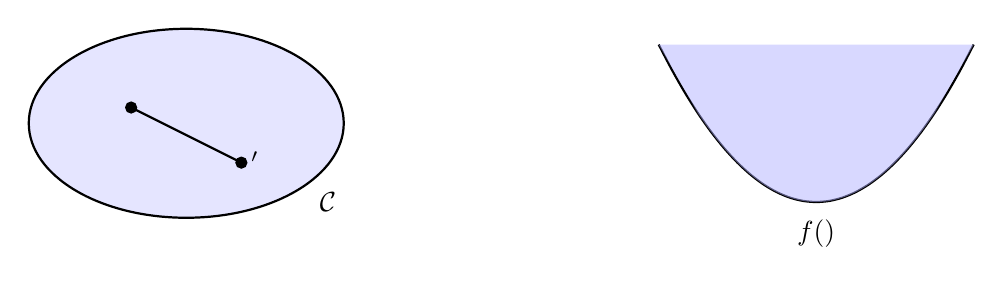
\begin{tikzpicture}
				% Left part: Convex set (Ellipse)
				\fill[blue!20, opacity=0.5] (-3,0) ellipse (2 and 1.2); % Shaded ellipse
				\draw[thick] (-3,0) ellipse (2 and 1.2);
			 % Points inside the ellipse
				\filldraw[black] (-3.7,0.2) circle (2pt) node[left] {$\vw$};
				\filldraw[black] (-2.3,-0.5) circle (2pt) node[right] {$\vw'$};
				% Line segment connecting the two points
				\draw[thick] (-3.7,0.2) -- (-2.3,-0.5);
				% Label for the convex set
				\node at (-1.2,-1.0) {$\mathcal{C}$};
				% Right part: Convex function and epigraph
				\begin{scope}[shift={(5,-1)}]
					% Define the convex function
					\draw[thick, domain=-2:2, smooth, variable=\x] 
					plot ({\x}, {0.5*\x*\x});
					% Shaded epigraph (area above the function)
					\fill[blue!30, opacity=0.5] 
					plot[domain=-1.5:1.5, smooth] ({\x}, {0.5*\x*\x}) -- 
					(2, {0.5*2*2}) -- 
					(-2, {0.5*2*2}) -- 
					cycle;
					%\fill[blue!30, opacity=0.5] (-1.5,1.2) -- (-1.5,2.5) -- (1.5,2.5) -- (1.5,1.2) -- plot[domain=-1.5:1.5, smooth] ({\x}, {0.5*\x*\x}) -- cycle;
					% Labels
					\node at (0,-0.4) {$f(\weights)$};
				\end{scope}
			\end{tikzpicture}
			\vspace*{-8mm}
			\end{center}
			\caption{Left: A convex set $\cluster \subseteq \mathbb{R}^{\dimlocalmodel}$. 
				Right: A convex function $f: \mathbb{R}^{\dimlocalmodel} \rightarrow \mathbb{R}$.\label{fig_convex_set_function}}
		\end{figure}},first={convex},text={convex}}


\newglossaryentry{smooth}{name={smooth},
	description={A\index{smooth} real-valued function $f: \mathbb{R}^{\dimlocalmodel} \rightarrow \mathbb{R}$ 
		is smooth if it is \gls{differentiable} and its \gls{gradient} $\nabla f(\weights)$ is continuous at all $\weights \in \mathbb{R}^{\dimlocalmodel}$  \cite{nesterov04,CvxBubeck2015}. A smooth function $f$ is referred to as $\beta$-smooth if the \gls{gradient} 
		$\nabla f(\weights)$ is Lipschitz continuous with Lipschitz constant $\beta$, i.e., 
		$$\| \nabla f(\weights) - \nabla f(\weights') \| \leq \beta \| \weights - \weights' \| \mbox{, for any } \weights,\weights' \in \mathbb{R}^{\dimlocalmodel}.$$ 
		The constant $\beta$ quantifies the amount of smoothness of the function $f$: the smaller the $\beta$, 
		the smoother $f$ is. Optimization problems with a smooth \gls{objfunc} can be solved effectively by \gls{gdmethods}. 
	    Indeed, \gls{gdmethods} approximate the \gls{objfunc} locally around a current choice $\weights$ 
	    using its \gls{gradient}. This approximation works well if the \gls{gradient} does 
	    not change too rapidly. We can make this informal claim precise by studying the effect of a single 
	    \gls{gradstep} with \gls{stepsize} $\lrate=1/\beta$ (see Figure \ref{fig_gd_smooth_dict}). 
	    \begin{figure}[H] 
	    	\begin{center} 
	    	\begin{tikzpicture}[scale=0.8, x=0.7cm,y=0.05cm]
	    		% Parameter to shift the quadratic curve horizontally
	    		\def\hshift{0.5} % Change this value to shift the curve horizontally
	    		% Define the function (only the increasing part of x^2 for x >= 0)
	    		\draw[thick, domain=\hshift:8+\hshift, smooth, variable=\x] plot ({\x}, {\x^2}); %node[right] {$f(x) = x^2$};
	    		% Define points for the tangents
	    		\coordinate (w) at (\hshift,{\hshift*\hshift}); % Point w on the curve (left end of the plot)
	    		\coordinate (wkplus1) at (4+\hshift,{(4+\hshift)^2}); % Point w^{k+1} on the curve (x=1 + hshift, y=1)
	    		\coordinate (wk) at (8+\hshift,{(8+\hshift)^2}); % Point w^k on the curve (right end of the plot)
	    		% Calculate the slopes for the tangents
  				\draw[line width=1pt, transform canvas={yshift=-2pt}] (wk) -- +(-1, -{2*(8 + \hshift)} ) -- +(1, {2*(8 + \hshift)}); % Tangent at w^k with positive slope
 				\draw[line width=1pt, transform canvas={yshift=-2pt}] (w) -- +(-1, -{2*\hshift} ) -- +(1, {2*\hshift} )  node[below] {$\nabla f(\weights)$};% Tangent at w with slope 0 (since derivative at hshift = 0)
%	    		% Draw filled circles at points w^k, w, and w^{k+1}
	    		\filldraw (wk) circle (2pt) node[above left] {$\weights^{(\iteridx)}$} node[below right] {$\nabla f(\weights^{(\iteridx)})$} ;
	    		\filldraw (w) circle (2pt) node[above right] {$\weights$} ;
	    		\filldraw (wkplus1) circle (2pt) node[below right] {$\weights^{(\iteridx+1)}\!=\!\weights^{(\iteridx)}\!-\!(1/\beta)\nabla f(\weights^{(\iteridx)})$};
	    		    % Draw horizontal rulers to mark the function values at wk and wk_plus1
	    		\draw[dashed] (wk) -- ($(8,0) + (wk)$) ; %node[left] {$f(\weights^{(\iteridx)})$};
	    		\draw[dashed] (wkplus1) -- ($(12,0) + (wkplus1)$) ; %node[left] {$f(\weights^{(\iteridx+1)})$};
	    		 \draw[<->, thick] ($(4,0) + (wk)$) -- ($(8,0) + (wkplus1)$) 
	    		node[midway, right] {$ f\big(\weights^{(\iteridx)}\big)\!-\!f\big(\weights^{(\iteridx+1)}\big)\!\geq\!\frac{1}{2\beta}\normgeneric{\nabla f(\weights^{(\iteridx)})}{2}^{2}$};
%	    		% Label the curve
%	    		\node at (2, 4) {};
	    	\end{tikzpicture}
	    	\end{center}
	    	\caption{Consider an \gls{objfunc} $f(\weights)$ that is $\beta$-smooth. 
	    		Taking a \gls{gradstep}, with \gls{stepsize} $\lrate = 1/\beta$, decreases the 
	    		objective by at least $\frac{1}{2\beta}\normgeneric{\nabla f(\weights^{(\iteridx)})}{2}^{2}$ \cite{nesterov04,CvxAlgBertsekas,CvxBubeck2015}. 
	    		Note that the \gls{stepsize} $\lrate = 1/\beta$ becomes larger for smaller $\beta$. Thus, 
	    		for smoother \gls{objfunc}s (i.e., those with smaller $\beta$), 
				we can take larger steps. \label{fig_gd_smooth_dict}}
	    	\end{figure}
	    },first={smooth},text={smooth}}

\newglossaryentry{paramspace}{name={parameter space},
		description={The\index{parameter space} parameter space $\paramspace$ of 
		an \gls{ml} \gls{model} $\hypospace$ is the set of all feasible choices for the 
		\gls{modelparams} (see Figure \ref{fig_param_space_dict}). Many important \gls{ml} methods 
		use a \gls{model} that is parametrized by vectors of the \gls{euclidspace} $\mathbb{R}^{\dimlocalmodel}$. 
		Two widely used examples of parametrized \gls{model}s are \gls{linmodel}s 
		and \gls{deepnet}s. The parameter space is then often a subset $\paramspace \subseteq \mathbb{R}^{\dimlocalmodel}$, 
		e.g., all vectors $\weights \in \mathbb{R}^{\dimlocalmodel}$ with a \gls{norm} smaller than one.
		\begin{figure}[H]
			\begin{center}
			\begin{tikzpicture}
				% Left part: Ellipse representing parameter space (with two dots)
				\node[ellipse, minimum width=3cm, minimum height=2cm, draw, thick] (paramspace) {};
				\node[below=0.1cm of paramspace] {parameter space $\paramspace$};
				% Two dots inside the left ellipse
				\node[black, circle, inner sep=2pt, fill] (theta1) at ($(paramspace.north west) + (1, -1)$) {};
				\node[left=0.01cm of theta1] {$\weights$};
				\node[black, circle, inner sep=2pt, fill] (theta2) at ($(paramspace.south east) + (-1.5, 1)$) {};
				\node[left=0.01cm of theta2] {$\weights'$};
				% Right part: Ellipse containing two smaller plots
				\node[ellipse, minimum width=7cm, minimum height=3cm, draw, thick, right=4cm of paramspace] (plotcloud) {};
				\node[above=0.2cm of plotcloud] {\gls{model} $\hypospace$};
				% Axis for first smaller plot
				\node (plot1start) at ($(plotcloud.south west) + (0.2, 0.2)$) {};
				%\draw[thick, ->] (plot1start) -- ++(2, 0) node[anchor=north] {$\featurevec$};
				%\draw[thick, ->] (plot1start) -- ++(0, 1.5) node[anchor=east] {$\truelabel$};
				% Simple plot line in first smaller plot
				\draw[thick, red] (plot1start) .. controls ++(0.8, 1) and ++(-0.8, -0.8) .. ($(plotcloud.south west) + (2.8, 0.8)$) node[anchor=west] {$\hypothesis^{(\weights)}$};
				% Axis for second smaller plot
				\node (plot2start) at ($(plotcloud.south west) + (1.0, 1.2)$) {};
			%	\draw[thick, ->] (plot2start) -- ++(2, 0) node[anchor=north] {$\featurevec$};
			%	\draw[thick, ->] (plot2start) -- ++(0, 1.5) node[anchor=east] {$\truelabel$};
				% Simple plot line in second smaller plot
				\draw[thick, blue] (plot2start) .. controls ++(0.8, 0.5) and ++(-0.8, -0.8) .. ($(plotcloud.south west) + (2.8, 2.1)$) node[anchor=west] {$\hypothesis^{(\weights')}$};
				% Connect the two dots in the parameter space to the two plots
				\draw[thick, ->, bend right=20] (theta1) to ($(plot1start) + (0,0)$);
				\draw[thick, ->, bend left=20] (theta2) to (plot2start);
			\end{tikzpicture}
			\end{center} 
			\caption{The parameter space $\paramspace$ of an \gls{ml} \gls{model} $\hypospace$ consists of all 
			feasible choices for the \gls{modelparams}. Each choice $\weights$ for the \gls{modelparams} 
			selects a \gls{hypothesis} map $\hypothesis^{(\weights)} \in \hypospace$.
				 \label{fig_param_space_dict}} 
\end{figure}},
			first={parameter space},text={parameter space}}

\newglossaryentry{datanorm}{name={data normalization},
	description={\Gls{data} normalization\index{data normalization} refers to transformations 
		applied to the \gls{featurevec}s of \gls{datapoint}s to improve the \gls{ml} method's 
		\gls{statasp} or \gls{compasp}. For example, in \gls{linreg} with \gls{gdmethods} using 
		a fixed \gls{learnrate}, convergence depends on controlling the \gls{norm} of \gls{featurevec}s 
		in the \gls{trainset}. A common approach is to normalize \gls{featurevec}s such that their 
		\gls{norm} does not exceed one \cite[Ch.\ 5]{MLBasics}.},
	first={data normalization},text={data normalization}}

\newglossaryentry{dataaug}{name={data augmentation},
	description={\Gls{data} augmentation\index{data augmentation} methods add synthetic \gls{datapoint}s 
		to an existing set of \gls{datapoint}s. These synthetic \gls{datapoint}s are obtained by 
		perturbations (e.g., adding noise to physical measurements) or transformations 
		(e.g., rotations of images) of the original \gls{datapoint}s. These perturbations and 
		transformations are such that the resulting synthetic \gls{datapoint}s should 
		still have the same \gls{label}. As a case in point, a rotated cat image is still 
		a cat image even if their \gls{featurevec}s (obtained by stacking pixel color intensities) 
		are very different (see Figure \ref{fig_symmetry_dataaug_dict}). \Gls{data} augmentation can be an 
		efficient form of \gls{regularization}.
		\begin{figure}[H]
		\begin{center}
			\begin{tikzpicture}
				% Define shift macros locally
				\newcommand{\xshift}{0.5}
				\newcommand{\yshift}{2}
				% Define the shifted curves
				% Define the shifted curves
  				\draw[very thick, blue] plot[smooth, tension=1] coordinates {(0,0) (2,1) (4,0) (6,-1) (8,0)};
  				\node[blue, right] at (0,0) {\textbf{cat}};
  				\draw[very thick, red, dashed] plot[smooth, tension=1] coordinates {(0 + \xshift,0 + \yshift) (2 + \xshift,1 + \yshift) (4 + \xshift,0 + \yshift) (6 + \xshift,-1 + \yshift) (8 + \xshift,0 + \yshift)};
  				\node[red, right] at (8 + \xshift,0 + \yshift) {\textbf{no cat}};
				\fill[blue] (2,1) circle (2pt) node[above] {$\featurevec^{(1)}$};
				\fill[blue] (6,-1) circle (2pt) node[above] {$\featurevec^{(2)}$};
				  % Draw a bent arrow connecting the two points with custom in and out angles
				  \draw[->, thin, >=latex, line width=0.5pt] (2,1) to[out=240, in=240] node[midway, below] {$\mathcal{T}^{(\eta)}$} (6,-1);
			  \end{tikzpicture}
			  \vspace*{-11mm}
		\end{center}
		\caption{\Gls{data} augmentation exploits intrinsic symmetries of \gls{datapoint}s in 
		       some \gls{featurespace} $\featurespace$. We can represent a symmetry by 
		     an operator $\mathcal{T}^{(\eta)}: \featurespace \rightarrow \featurespace$,
		     parametrized by some number $\eta \in \mathbb{R}$. For example, $\mathcal{T}^{(\eta)}$ 
		    might represent the effect of rotating a cat image by $\eta$ degrees. A \gls{datapoint} 
		    with \gls{featurevec} $\featurevec^{(2)} = \mathcal{T}^{(\eta)} \big(\featurevec^{(1)} \big)$ must 
		    have the same \gls{label} $\truelabel^{(2)}=\truelabel^{(1)}$ as a \gls{datapoint} 
		     with \gls{featurevec} $\featurevec^{(1)}$.\label{fig_symmetry_dataaug_dict}}
		 \end{figure} },first={data augmentation},text={data augmentation}}
	
	
\newglossaryentry{localdataset}{name={local dataset},description={The\index{local dataset} concept of a local \gls{dataset} is 
		in between the concept of a \gls{datapoint} and a \gls{dataset}. A local \gls{dataset} consists of several 
		individual \gls{datapoint}s, which are characterized by \gls{feature}s and \gls{label}s. 
		In contrast to a single \gls{dataset} used in basic \gls{ml} methods, a local \gls{dataset} is also 
		related to other local \gls{dataset}s via different notions of similarity. These similarities 
		might arise from \gls{probmodel}s or communication infrastructure and 
		are encoded in the edges of an \gls{empgraph}.},first={local dataset},text={local dataset}}
	
\newglossaryentry{localmodel}{name={local model},description={Consider\index{local model} a collection 
		of \gls{localdataset}s that are assigned to the nodes of an \gls{empgraph}. A local \gls{model} $\localmodel{\nodeidx}$ 
		is a \gls{hypospace} assigned to a node $\nodeidx \in \nodes$. Different nodes might be assigned 
		different \gls{hypospace}s, i.e., in general $\localmodel{\nodeidx} \neq \localmodel{\nodeidx'}$ for different 
		nodes $\nodeidx, \nodeidx' \in \nodes$.  },first={local model},text={local model}}
	
\newglossaryentry{mutualinformation}
{name={mutual information (MI)},
 description={The\index{mutual information (MI)} MI $\mutualinformation{\featurevec}{\truelabel}$ 
 	between two \gls{rv}s $\featurevec$, $\truelabel$ defined on the same \gls{probspace} 
 	is given by \cite{coverthomas} $$\mutualinformation{\featurevec}{\truelabel} \defeq 
	\expect \left\{ \log \frac{p (\featurevec,\truelabel)}{p(\featurevec)p(\truelabel)} \right\}.$$ 
	It is a measure of how well we can estimate $\truelabel$ based 
	solely on $\featurevec$. A large value of $\mutualinformation{\featurevec}{\truelabel}$ indicates that 
	$\truelabel$ can be well predicted solely from $\featurevec$. This \gls{prediction} could be obtained by a 
		\gls{hypothesis} learned by an \gls{erm}-based \gls{ml} method. 
	 }, first={MI}, text={MI} 
}

\newglossaryentry{zerogradientcondition}{name={zero-gradient condition},
	description={Consider\index{zero-gradient condition} the unconstrained 
		optimization problem $\min_{\weights \in \mathbb{R}^{\dimlocalmodel}} f(\weights)$  with 
			a \gls{smooth} and \gls{convex} \gls{objfunc} $f(\weights)$. A necessary and 
			sufficient condition for a vector $\widehat{\weights} \in \mathbb{R}^{\dimlocalmodel}$ 
			to solve this problem is that the \gls{gradient} $\nabla f \big( \widehat{\weights} \big)$ 
			is the zero vector, 
			$$ \nabla f \big( \widehat{\weights} \big) = \mathbf{0} \Leftrightarrow  f \big( \widehat{\weights} \big) = \min_{\weights \in \mathbb{R}^{\dimlocalmodel}} f(\weights) .$$ }, 
			first={zero-gradient condition},text={zero-gradient condition}}


\newglossaryentry{edgeweight}{name={edge weight},
	description={Each\index{edge weight} edge $\edge{\nodeidx}{\nodeidx'}$ of an \gls{empgraph} is 
		assigned a non-negative edge weight $\edgeweight_{\nodeidx,\nodeidx'}\geq0$. 
		A zero edge weight $\edgeweight_{\nodeidx,\nodeidx'}=0$ indicates the absence 
		of an edge between nodes $\nodeidx, \nodeidx' \in \nodes$.}, 
	first={edge weight},text={edge weight}}


\newglossaryentry{dataminprinc}{name={data minimization principle},
	description={European\index{data minimization principle} \gls{data} protection regulation 
		includes a \gls{data} minimization principle. This principle requires a \gls{data} controller to 
		limit the collection of personal information to what is directly relevant and necessary 
		to accomplish a specified purpose. The \gls{data} should be retained only for as long as 
		necessary to fulfill that purpose \cite[Article 5(1)(c)]{GDPR2016}, \cite{EURegulation2018}.}, 
	first={data minimization principle},text={data minimization principle}}


